%*******************************************************************************
\documentclass[fleqn,10pt]{wlscirep}
\usepackage[utf8]{inputenc}
\usepackage[T1]{fontenc}
\graphicspath{{../}} %%%REPOSITORY PATH

\title{The Application of Recurrent Quantification Analysis 
to Human-Humanoid Interaction}
\author[1,*]{Miguel Xochicale}
\author[1]{Chris Baber}
\affil[1]{University of Birmingham, 
	School of Engineering, 
	Birmingham, 
	B15 2TT, 
	UK}
\affil[*]{map479@bham.ac.uk}

%\keywords{Keyword1, Keyword2, Keyword3}

\begin{abstract}
Human movement variability occurs in motor performance 
across multiple repetitions of a task and such behaviour is an
inherent feature within and between each persons' movement. Quantifying
movement variability is still an open problem, particularly when traditional
methods in time domain and frequency domain fail to detect tiny modulations in
frequency or phase for time series. 
For this work, we hence investigate methodologies from nonlinear dynamics such as 
reconstructed state space (RSS), uniform time-delay embedding (UTDE), 
recurrence plots (RPs) and recurrence quantification analysis (RQA) metrics. 
Particularly, we are interested in the weaknesses and robustness 
of nonlinear dynamics tools from raw and post-processed data of 
wearable inertial sensors (IMUs). 
In the reported experiment, twenty right-handed healthy participants 
imitated simple vertical and horizontal arm movements in normal 
and faster speed from an humanoid robot.
With four window lengths and three levels of smoothed time series, 
we found visual differences in the patterns of RSSs and RPs. 
Then with the use of RQA metrics, we find out that the type of 
movements and the level of smoothness affects those metrics. 
Specifically, entropy values from RQA were well distributed and 
presented variation in all the conditions for time series. 
This work have then the potential to enhance the development of 
better diagnostic tools for various applications in rehabilitation, 
sport science or for new forms of human-robot interaction.
\end{abstract}
%226



\begin{document}

\flushbottom
\maketitle
\thispagestyle{empty}


\section*{Introduction}
Human movement requires a complex system where not only multiple
joints and limbs are involved for a specific task in a determined environment
but also perception and action of movement affects the physical performance 
\cite{davids2003}. 
In contrast, variability in humanoid movement is usually very small,
as a result of the control system used. This means that, while humanoids 
solve the degrees of freedom problem through join design and algorithms,
humans tend to have more fluid and flexible approach. Consequently, 
one can see much variability in the performance of even the simplest task.
Studies of human motion reveal the possibility to 
estimate features from lower dimension signals to distinguish differences between 
styles of pedalling motion \cite{Quintana-Duque2012, Quintana-Duque2016}, 
gait identification \cite{sama2013, frank2010},
and detection of pathologies \cite{gomezgarcia2014}.
The lower dimension signals from biological systems are time series 
of $1-$dimension in $\mathbb{R}$ which commonly are 
noisy, nonlinear and non-stationary \cite{gomezgarcia2014}.
Hence, nonlinear dynamics can be used to 
objectively quantify variability of lower
dimension signals \cite{Quintana-Duque2012, Quintana-Duque2016, sama2013, 
frank2010, gomezgarcia2014, marwan2011, stergiou2011}.
For instance, Bradley et al. 2015 \cite{bradley2015} reviewed methods for
nonlinear time series analysis based on the appropriate estimation of the 
embedding parameters ($m$ embedding dimension and $\tau$ embedding delay) to 
reconstruct the state space,
where an $n$-dimensional reconstructed state space using $1-$dimensional 
time series,
can preserve the topological properties of an unknown $M$-dimensional 
state space \cite{takens1981}.
Bradley et al. 2015 \cite{bradley2015} also reviewed the use of 
Recurrence Plots (RPs), a graphical representation of a two-dimensional map 
which show black and white dots as recurrences in a given $n$-dimensional system, 
and Recurrence Quantification Analysis (RQA) metrics compute statistics in RPs.
In general, RPs and RQA provide an intuitive meaning of the time series,
for instance, RQA is quantitatively and qualitatively independent of 
embedding dimension (also verified experimentally \cite{iwanski1998}).
However, the estimation of embedding parameters and the selection of the 
right parameters to perform RQA is still an open problem.
Bradley et al. 2015 \cite{bradley2015} pointed out that
there is no general technique that can be used to compute the embedding
parameters since time series are system-dependent which means that
computing the values for embedding parameters may only work for
one purpose (e.g., prediction) and may not work well for another purpose
(e.g., computing dynamical invariants).
Additionally, the methodologies of nonlinear dynamics for 
computing the embedding parameters e.g., autocorrelation, mutual information, 
and nearest neighbour require data which is well 
sampled and with little noise \cite{garland2016}
or require purely deterministic signals \cite{kantz2003}.
Thus, these nonlinear analysis methods for computing the embedding 
parameters can break down
with real-world datasets which have generally different length, 
different values of accuracy and precision (rounding errors due to finite 
precision of the measurement apparatus which include frequency 
acquisition \cite{frank2010}),
and data may be contaminated with different sources of noise
\cite{garland2016}.
It is surprising that even with the previous constraints with regard to 
the quality of data, and the problem with the estimation of embedding parameters,
the use of nonlinear dynamics have proven to be helpful to understand and 
characterise dynamics of time series 
\cite{Quintana-Duque2012, Quintana-Duque2016, sama2013, frank2010,
gomezgarcia2014, gomezgarcia2014, marwan2011, stergiou2011, bradley2015}.

%Another point to consider with time series analysis using nonlinear dynamics
%is the appropriate use of different post-processing techniques such as 
%interpolation, filtering or normalisation.
%With that in mind, it can be said that there is little research and 
%understanding on the effects for post-processing techniques
%in the interpretation of reconstructed state spaces, RPs and RQA.

For this work, we are interested in exploring and investigating  
the effects of different features of time series 
(e.g. levels of smoothness, window data length,
structures of time series based on types of movements, 
types of sensors, participants and velocities) to estimate 
embedded parameters for uniform time-delay embedding, 
recurrence plots and recurrence quantification analysis.
Hence, we conducted an experiment with twenty right-handed 
healthy participants in the context of human-humanoid imitation 
activities where participants were asked to 
imitate simple arm movements performed by a humanoid robot.
The primary aim of this work is to explore the following questions:
\begin{itemize}
\item What are the effects on three nonlinear methods 
	(reconstructed state space with uniform time-delay embedding, 
	Recurrence Plots, and Recurrence Quantification Analysis), 
	for different embedding parameters, different recurrence thresholds 
	and different characteristics of time series 
	(structure of the signal, window length and smoothness of the signal)?, and 
\item What are the strengths and weaknesses of Recurrence
	Quantification Analysis for the previous conditions
	of nonlinear analysis methods?
\end{itemize}


%*******************************************************************************
%*******************************************************************************
%*******************************************************************************
\section*{Results}

\subsection*{Reconstructed State Spaces}
One of the challenges of the implementation of 
Uniform Time-Delay Embedding to Reconstructed State Spaces is the 
selection of embedding parameters because each time series is unique in 
terms of its structure (modulation of amplitude, frequency and phase) 
\cite{ frank2010, sama2013, bradley2015}.
With that in mind, the problem for this work is not to compute individual 
embedding parameters for each of the time series but to deal with a 
selecting of two parameters that can represent all the time series. 
Our solution for that problem was to compute a sample mean over all 
values in each of the conditions of the time series 
%of Figs~\ref{fig:ts}
for minimum dimension values and 
%Figs~\ref{fig:caoami} 
for minimum delay values as follows.
%, resulting in an average minimum embedding parameters 
%of ($\overline{m_0}=6$, $\overline{\tau_0}=8$).

\subsubsection*{Minimum embedding parameters}
Minimum embedding parameters were firstly computed 
with False Nearest Neighbour and Average Mutual Information.
%for Uniform Time-Delay Embedding (UTDE),
%Reconstructed State Space (RSS), 
%Recurrence Plots (RPs) and 
%Recurrence Quantification Analysis (RQAs).
Figures \ref{fig:caoami}(A) show that minimum embedding values 
for sensor HS01 appear to show more variations as 
interquartile range is near to 1 
with three exceptions (HF sg0, VN sg0, and VF sg1).
Minimum embedding values appear to be constant for sensor RS01 
as interquartile range is near to 0.1 with the exception of 
two axis (HF sg0 and VF sg1).
Additionally, it can be seen in Figs \ref{fig:caoami}(A) a 
decrease of mean values (rhombus) in the box plots
as smoothness of time series increase.
Similarly, the first minimum values of AMI values are 
shown in the box plots of Figs \ref{fig:caoami}(B).
It can be seen that values for HS01 tend to be more spread as the smoothness 
of the time series is increasing 
(see the increase of both mean (rhombus) and interquartile range).
However, AMI values for RS01 do not show such increase in relation with
the increase of smoothness except for HF and VF
(Figs \ref{fig:caoami}(B)).

We also computed an overall minimum embedding parameters that represent 
participants, activities, sensors and levels of smoothness, using a sample 
mean of all values in Figs~\ref{fig:caoami}.
The sample mean for the minimum values of $E_{1}(m)$ from Figs \ref{fig:caoami}(A) 
is $\overline{m}_0=6$ 
and the sample mean for minimum values of AMIs from Figs~\ref{fig:caoami}(B)
is $\overline{\tau}_0=8$.
%Hence, we use the average minimum embedding parameters 
%($\overline{m_0}=6$, $\overline{\tau_0}=8$) to compute 
%Reconstructed State Spaces (RSSs), Recurrence Plots (RPs) and
%Recurrence Quantification Analysis (RQA) metrics for human-humanoid activities.
%---------------------------------(FIGURE)-------------------------------------
\begin{figure}[ht]
\centering
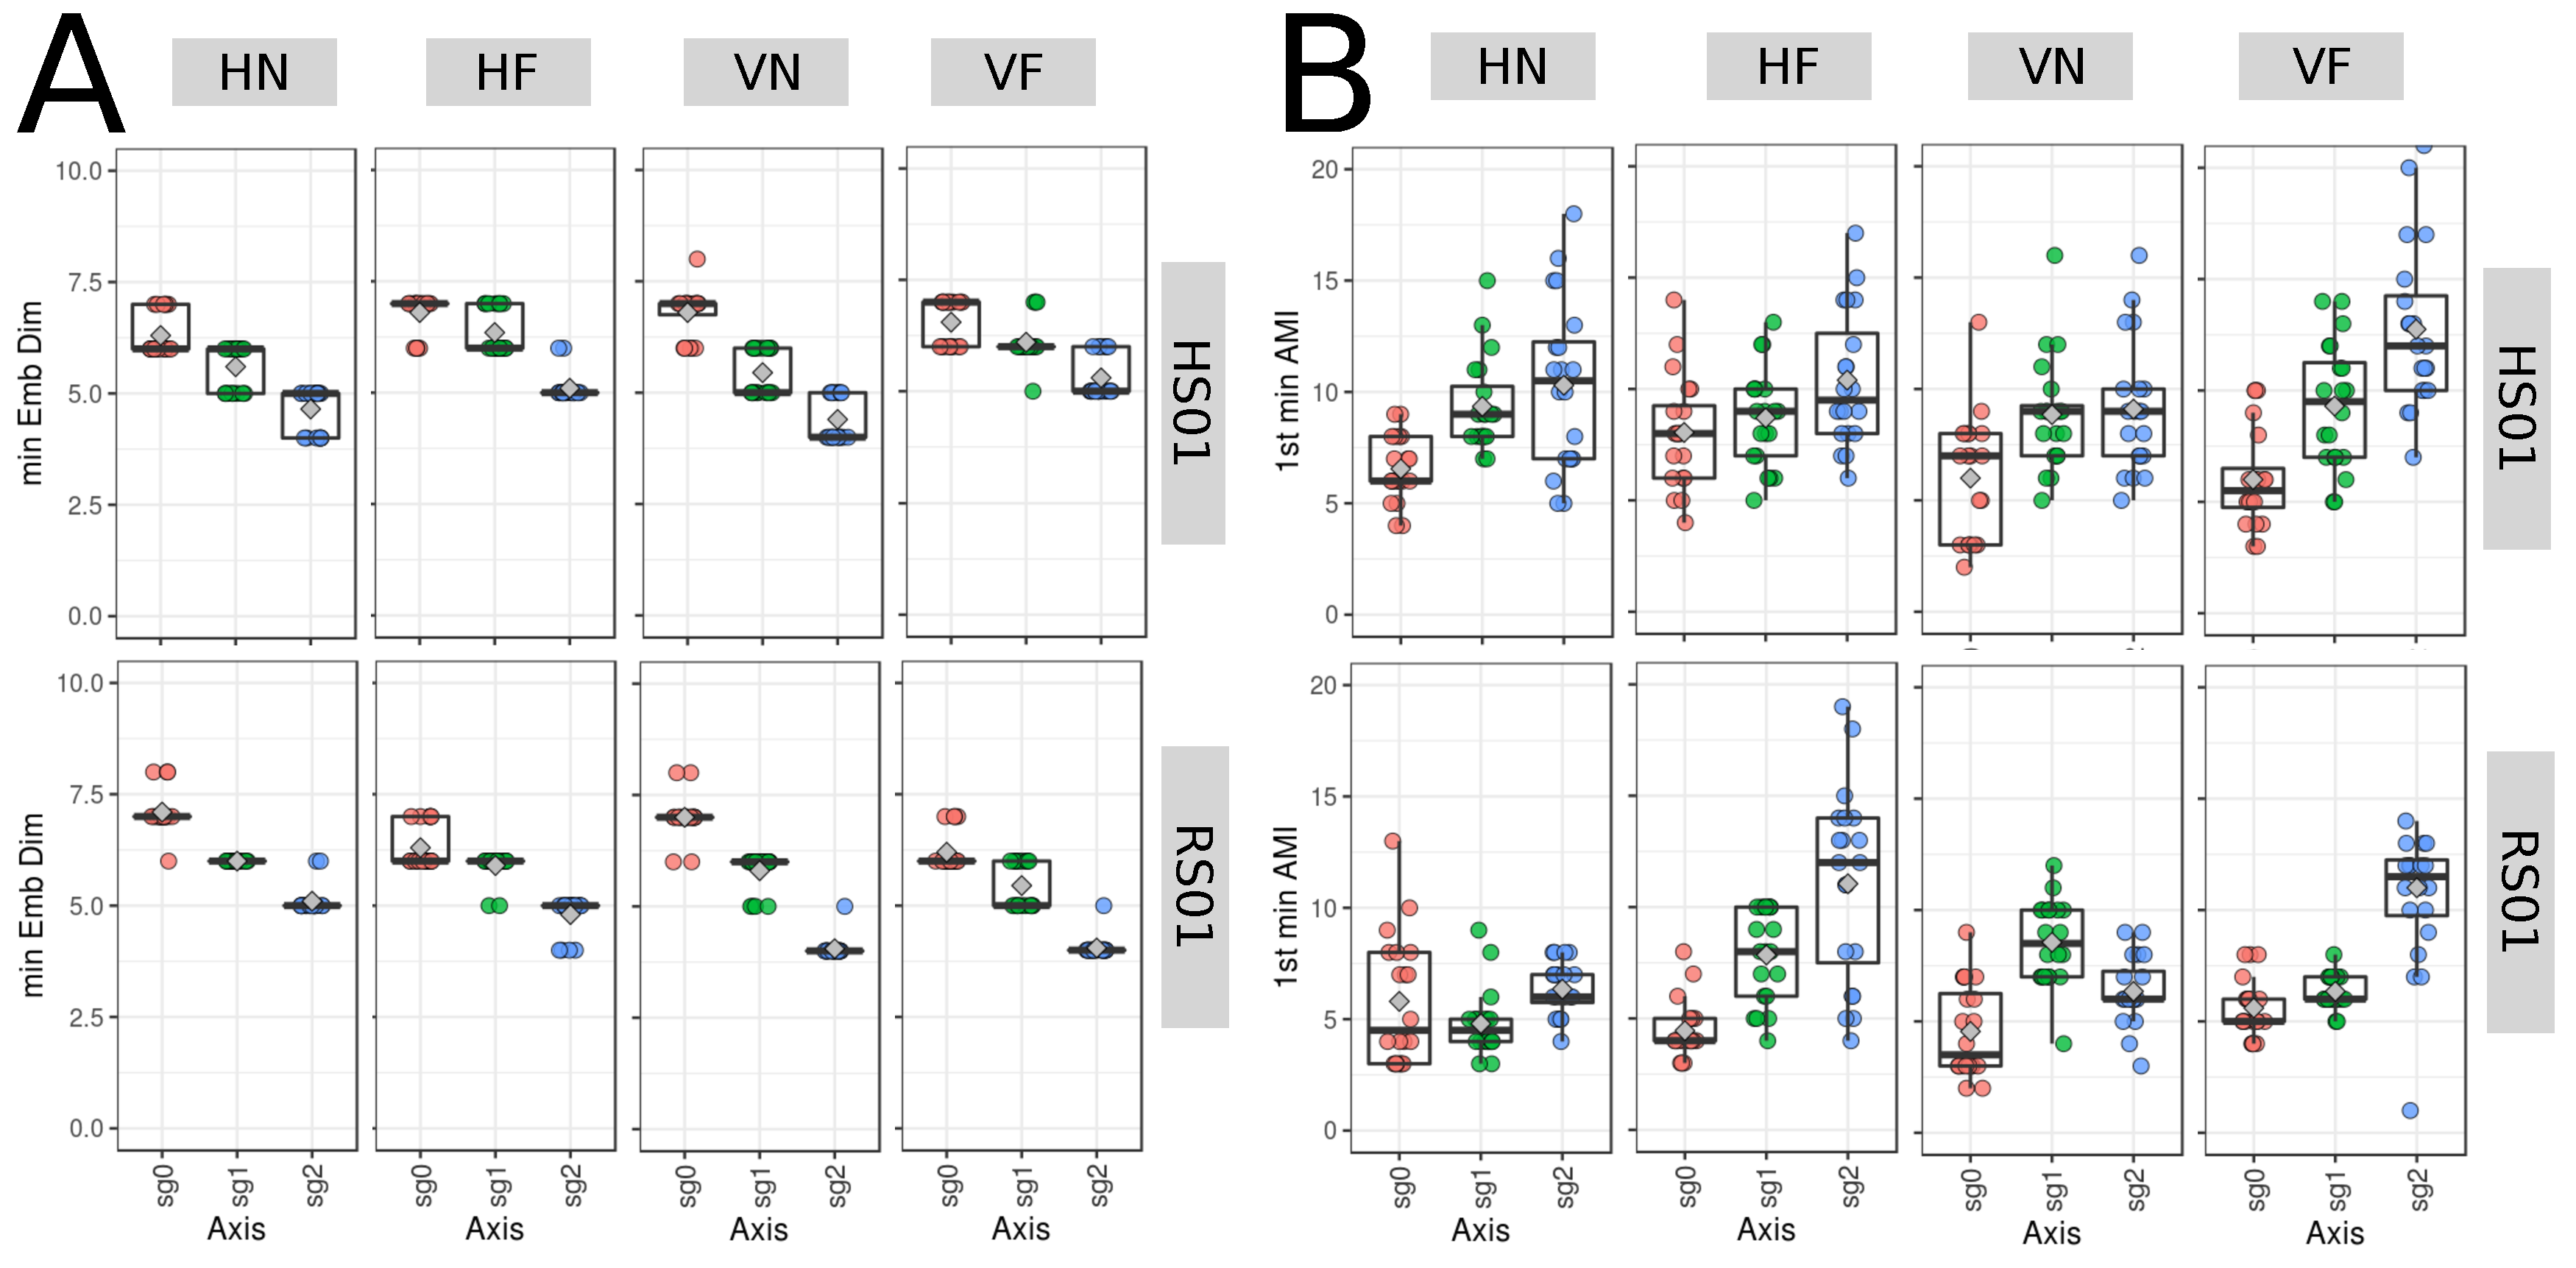
\includegraphics[width=1.0\textwidth]{figures/caoami/pdf/fig2}
	\caption{
	{\bf Box plots of minimum embedding parameters for horizontal and vertical arm movements.} 
	Box plots of (A) minimum embedding dimensions 
	and (B) first minimum AMI values for 
	Horizontal Normal (HN), Horizontal Faster (HF),
	Vertical Normal (VN) and Vertical Faster (VF)
	with sensors attached to participants (HS01) and
	sensor attached to robot (RS01).
	Minimum embedding dimensions are for twenty participants 
	($p01$ to $p20$) with three smoothed signals 
	(sg0: sg0zmuvGyroZ, sg1: sg1zmuvGyroZ and sg2: sg2zmuvGyroZ)
	and window length of 10-sec (500 samples).
	Code and data to reproduce the figure is available from \cite{srep2019}.
        }
    \label{fig:caoami}
\end{figure}
%%---------------------------------(FIGURE)------------------------------------


\subsubsection*{Uniform Time-Delay Embedding}
Uniform time-delay embedding were computed with
embedding parameters ($\overline{m_0}=6$, $\overline{\tau_0}=8$) and 
the first three axis of the rotated data of the PCA are shown 
for the reconstructed state spaces in 
Figs~\ref{fig:rss_aHw10} for horizontal arm movements and 
Figs~\ref{fig:rss_aVw10} for vertical arm movements.
%%---------------------------------(FIGURE)-------------------------------------
\begin{figure}[ht]
\centering
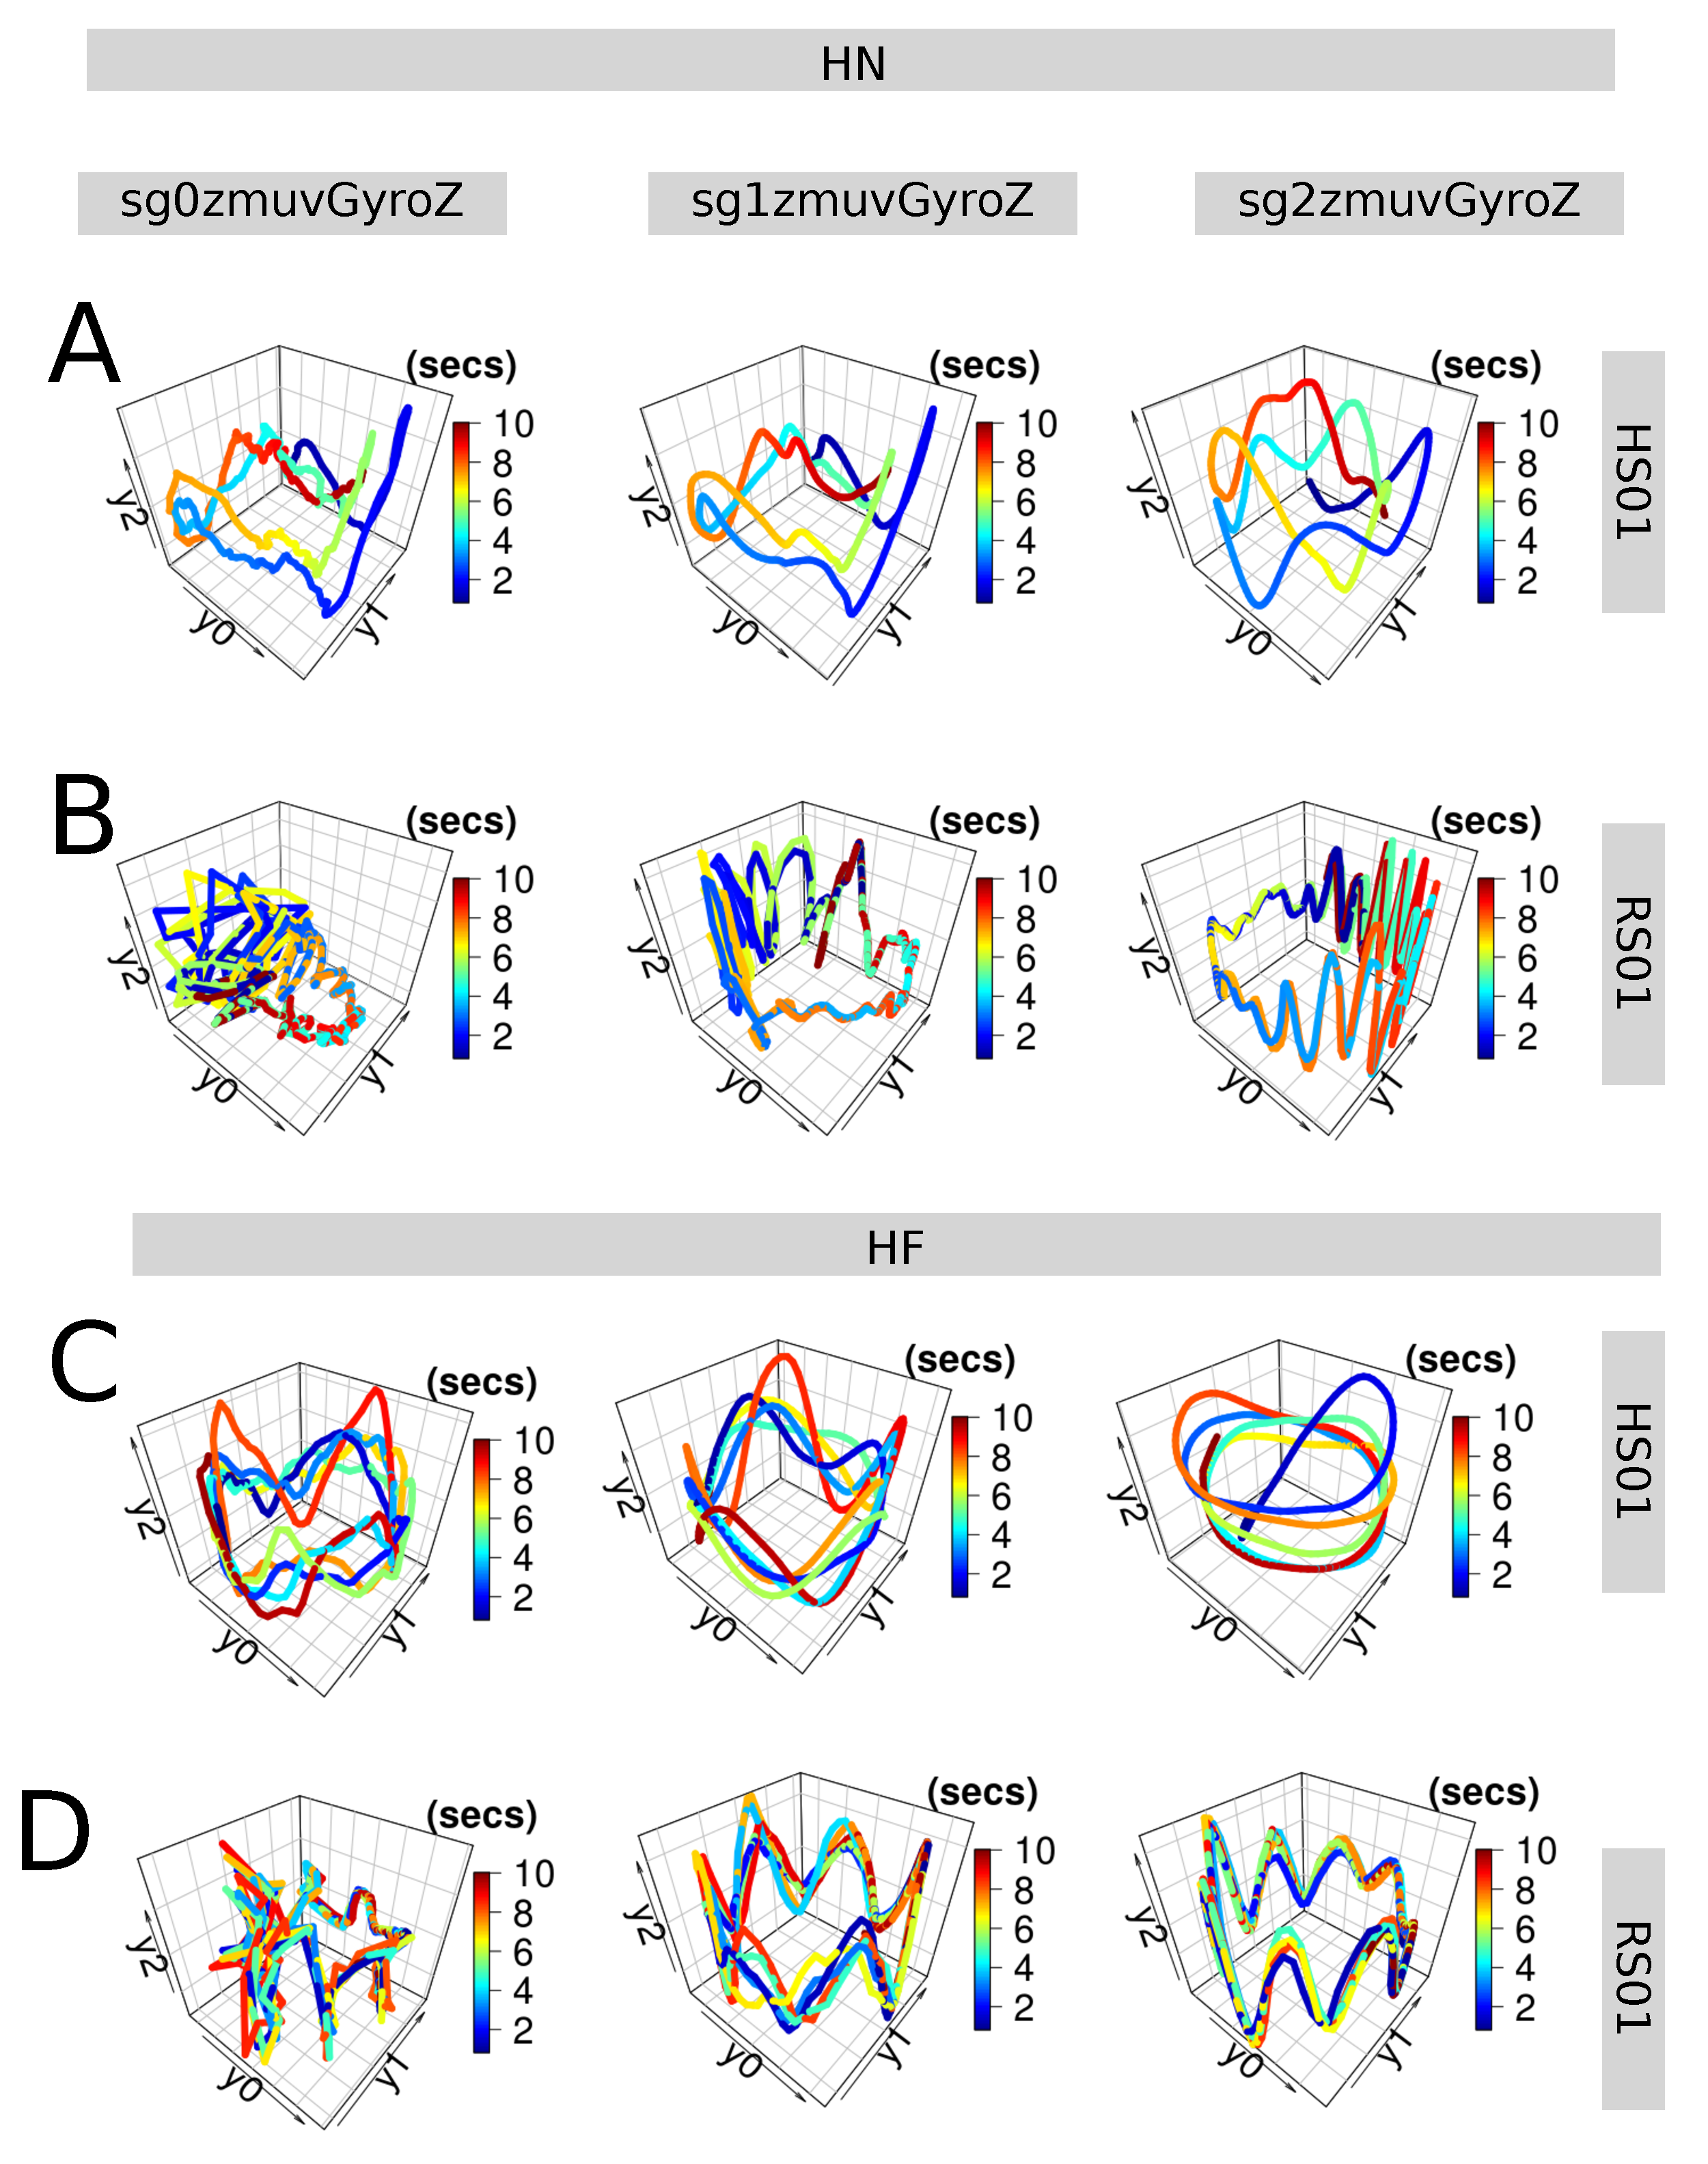
\includegraphics[width=1.0\textwidth]{figures/rss/pdf/fig3}
\caption{
	{\bf RSSs for horizontal arm movements.}
	Reconstructed state spaces for time series for p01 of Figure \ref{fig:ts}.
	Reconstructed state spaces were computed with 
	embedding parameters $m=6$, $\tau=8$.
	Code and data to reproduce the figure is available from \cite{srep2019}.
        }
    \label{fig:rss_aHw10}
\end{figure}
%%---------------------------------(FIGURE)------------------------------------
%%---------------------------------(FIGURE)-------------------------------------
\begin{figure}[ht]
\centering
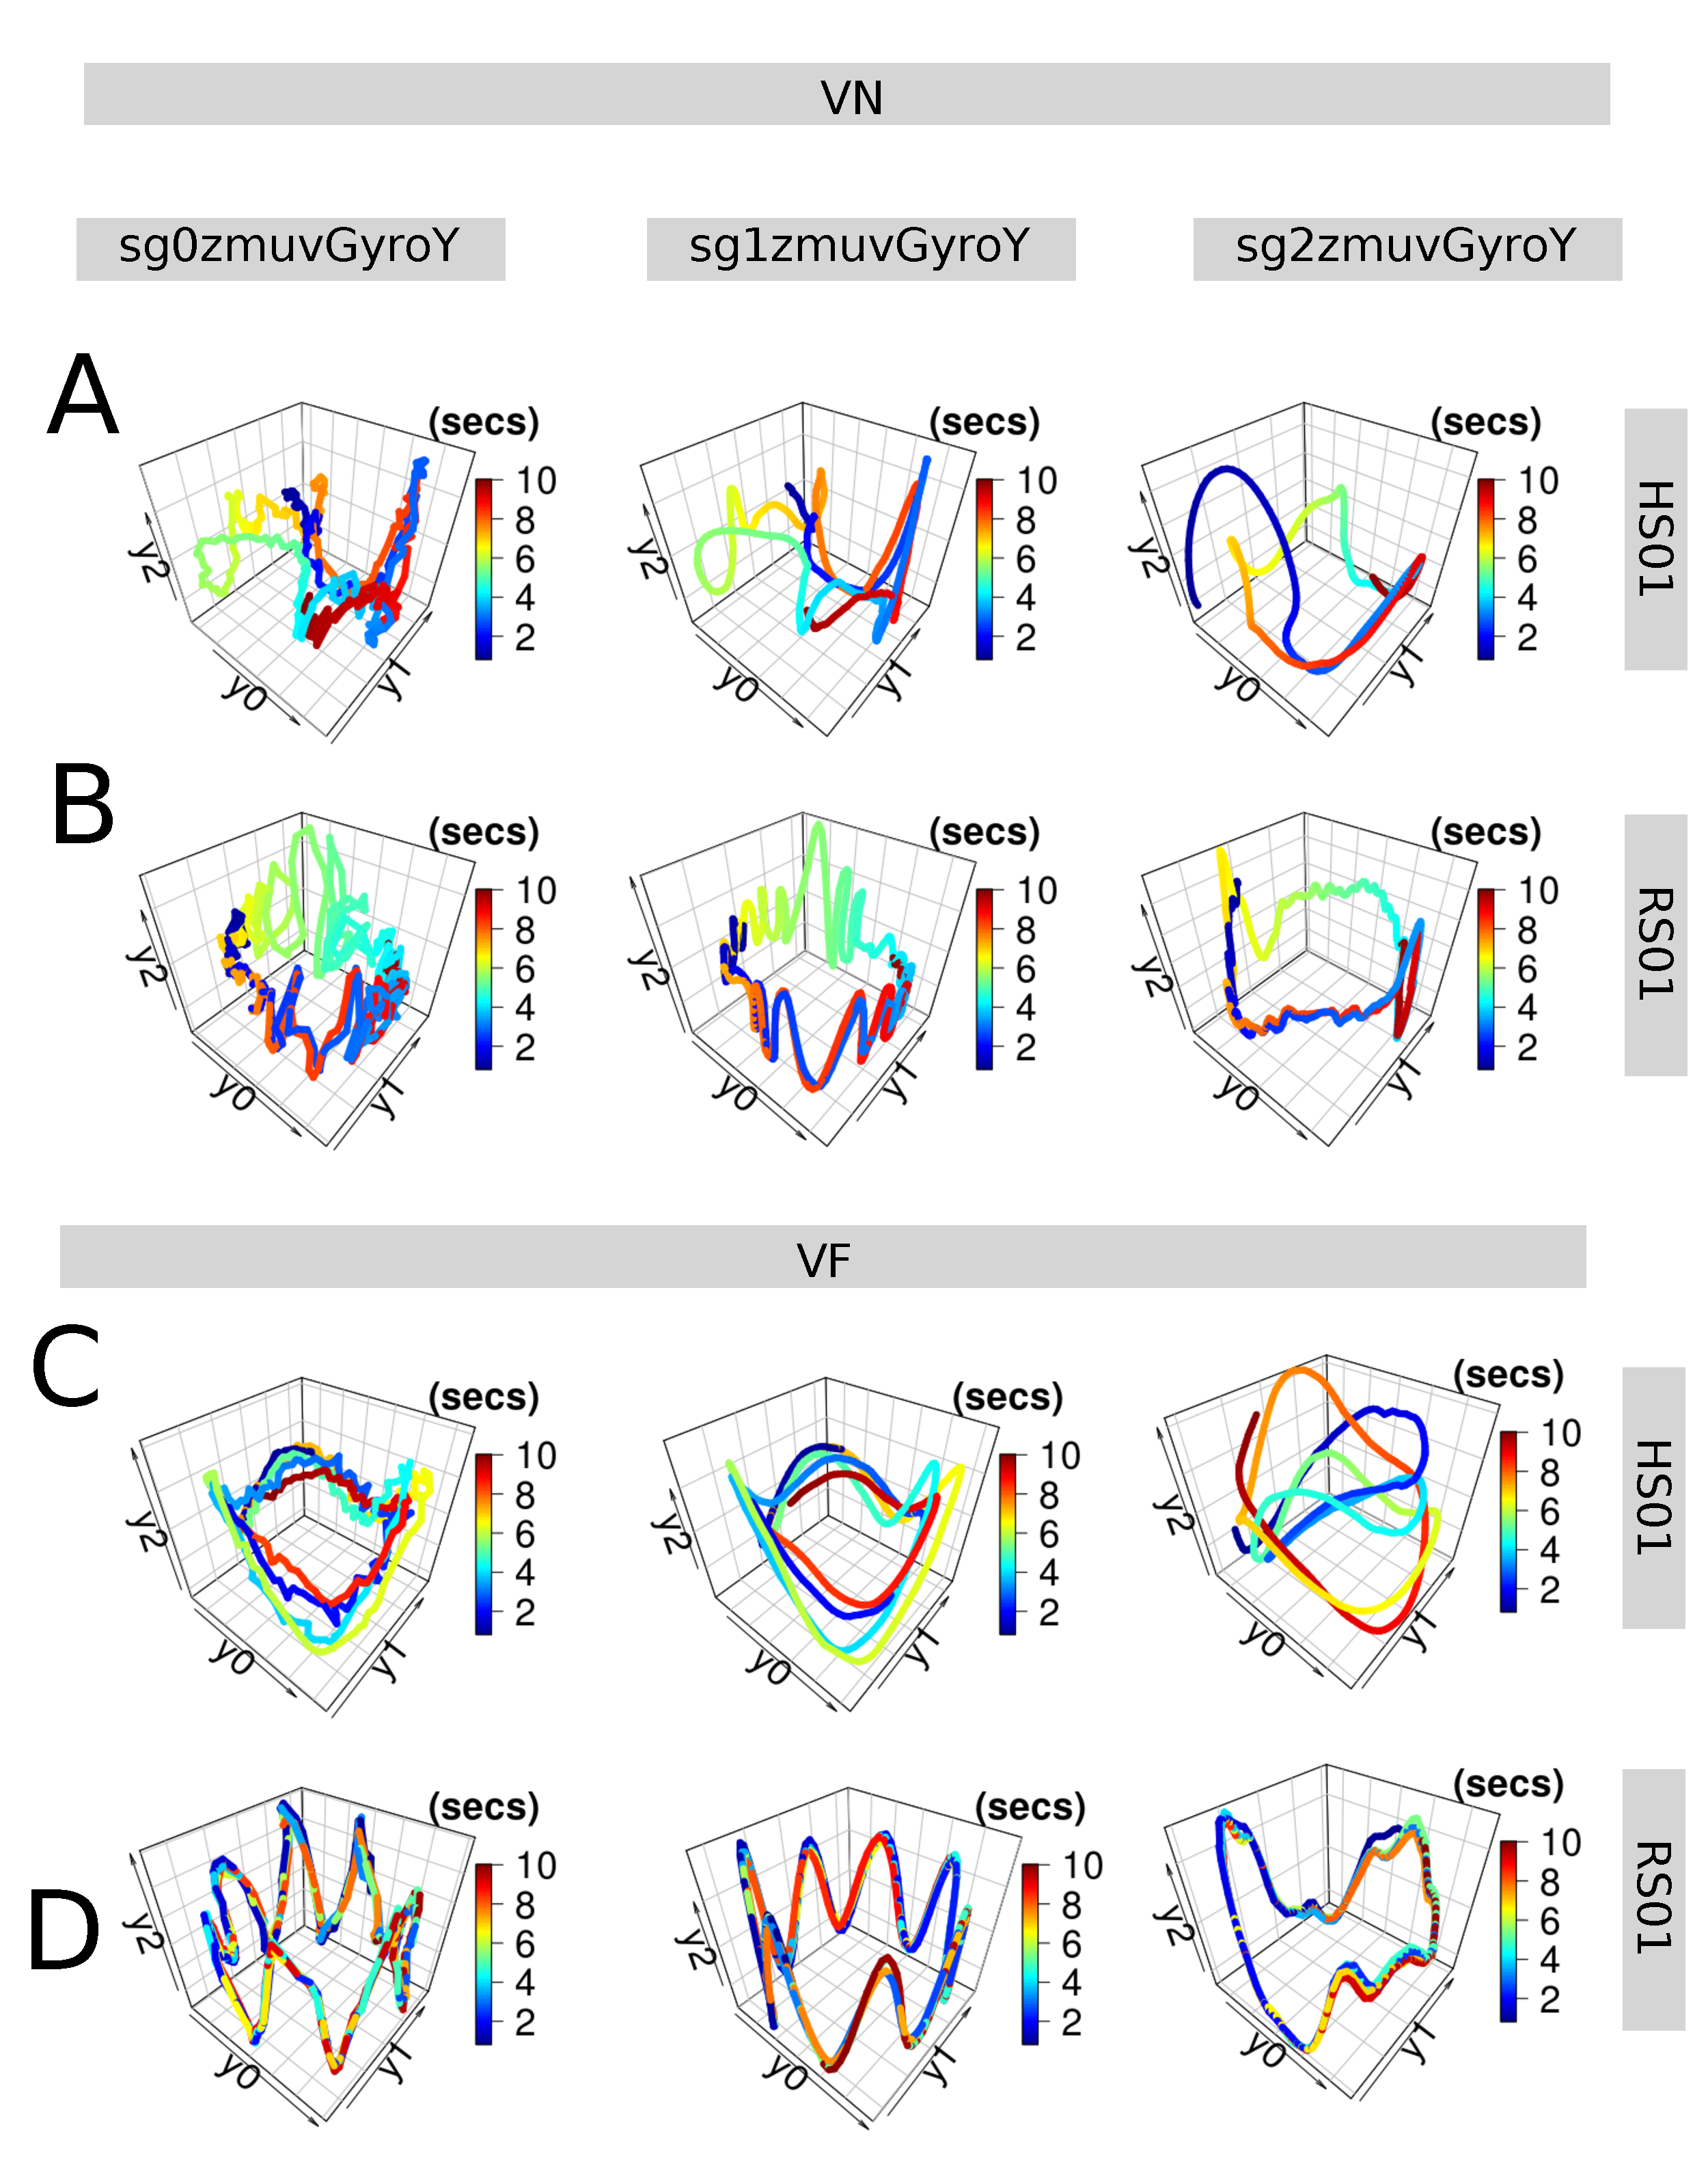
\includegraphics[width=1.0\textwidth]{figures/rss/pdf/fig4}
    \caption{
	{\bf RSSs for vertical arm movements.}
	Reconstructed state spaces for time series for p01 of Figure \ref{fig:ts}.
	Reconstructed state spaces were computed with 
	embedding parameters $m=6$, $\tau=8$.
	Code and data to reproduce the figure is available from \cite{srep2019}.
        }
    \label{fig:rss_aVw10}
\end{figure}
%%---------------------------------(FIGURE)------------------------------------

It is easy to observe by eye the differences in each of the
trajectories in the reconstructed state spaces 
(Figs~\ref{fig:rss_aHw10}, \ref{fig:rss_aVw10}), 
however one might be not objective when quantifying those differences 
since those observation might vary from person to person.
With that in mind, we tried to objectively quantify those differences 
using euclidean distances between the origin to each of the points in the 
trajectories, however these results created a suspicious metric, specially 
for trajectories which looked very messy.
With that in mind, we computed Recurrence Plots and 
Recurrence Quantification Analysis to objectively quantify 
the differences in each of the cases of the time series.




\subsection*{Recurrences Plots}
Recurrence Plots (RP) were computed for horizontal arm movements (Fig~\ref{fig:rp_aH}) and 
vertical arm movements (Fig~\ref{fig:rp_aV}) 
using the average embedding parameters ($m=6$, $\tau=8$) 
and an recurrence threshold of $\epsilon=1$.


%%---------------------------------(FIGURE)-------------------------------------
\begin{figure}[ht]
\centering
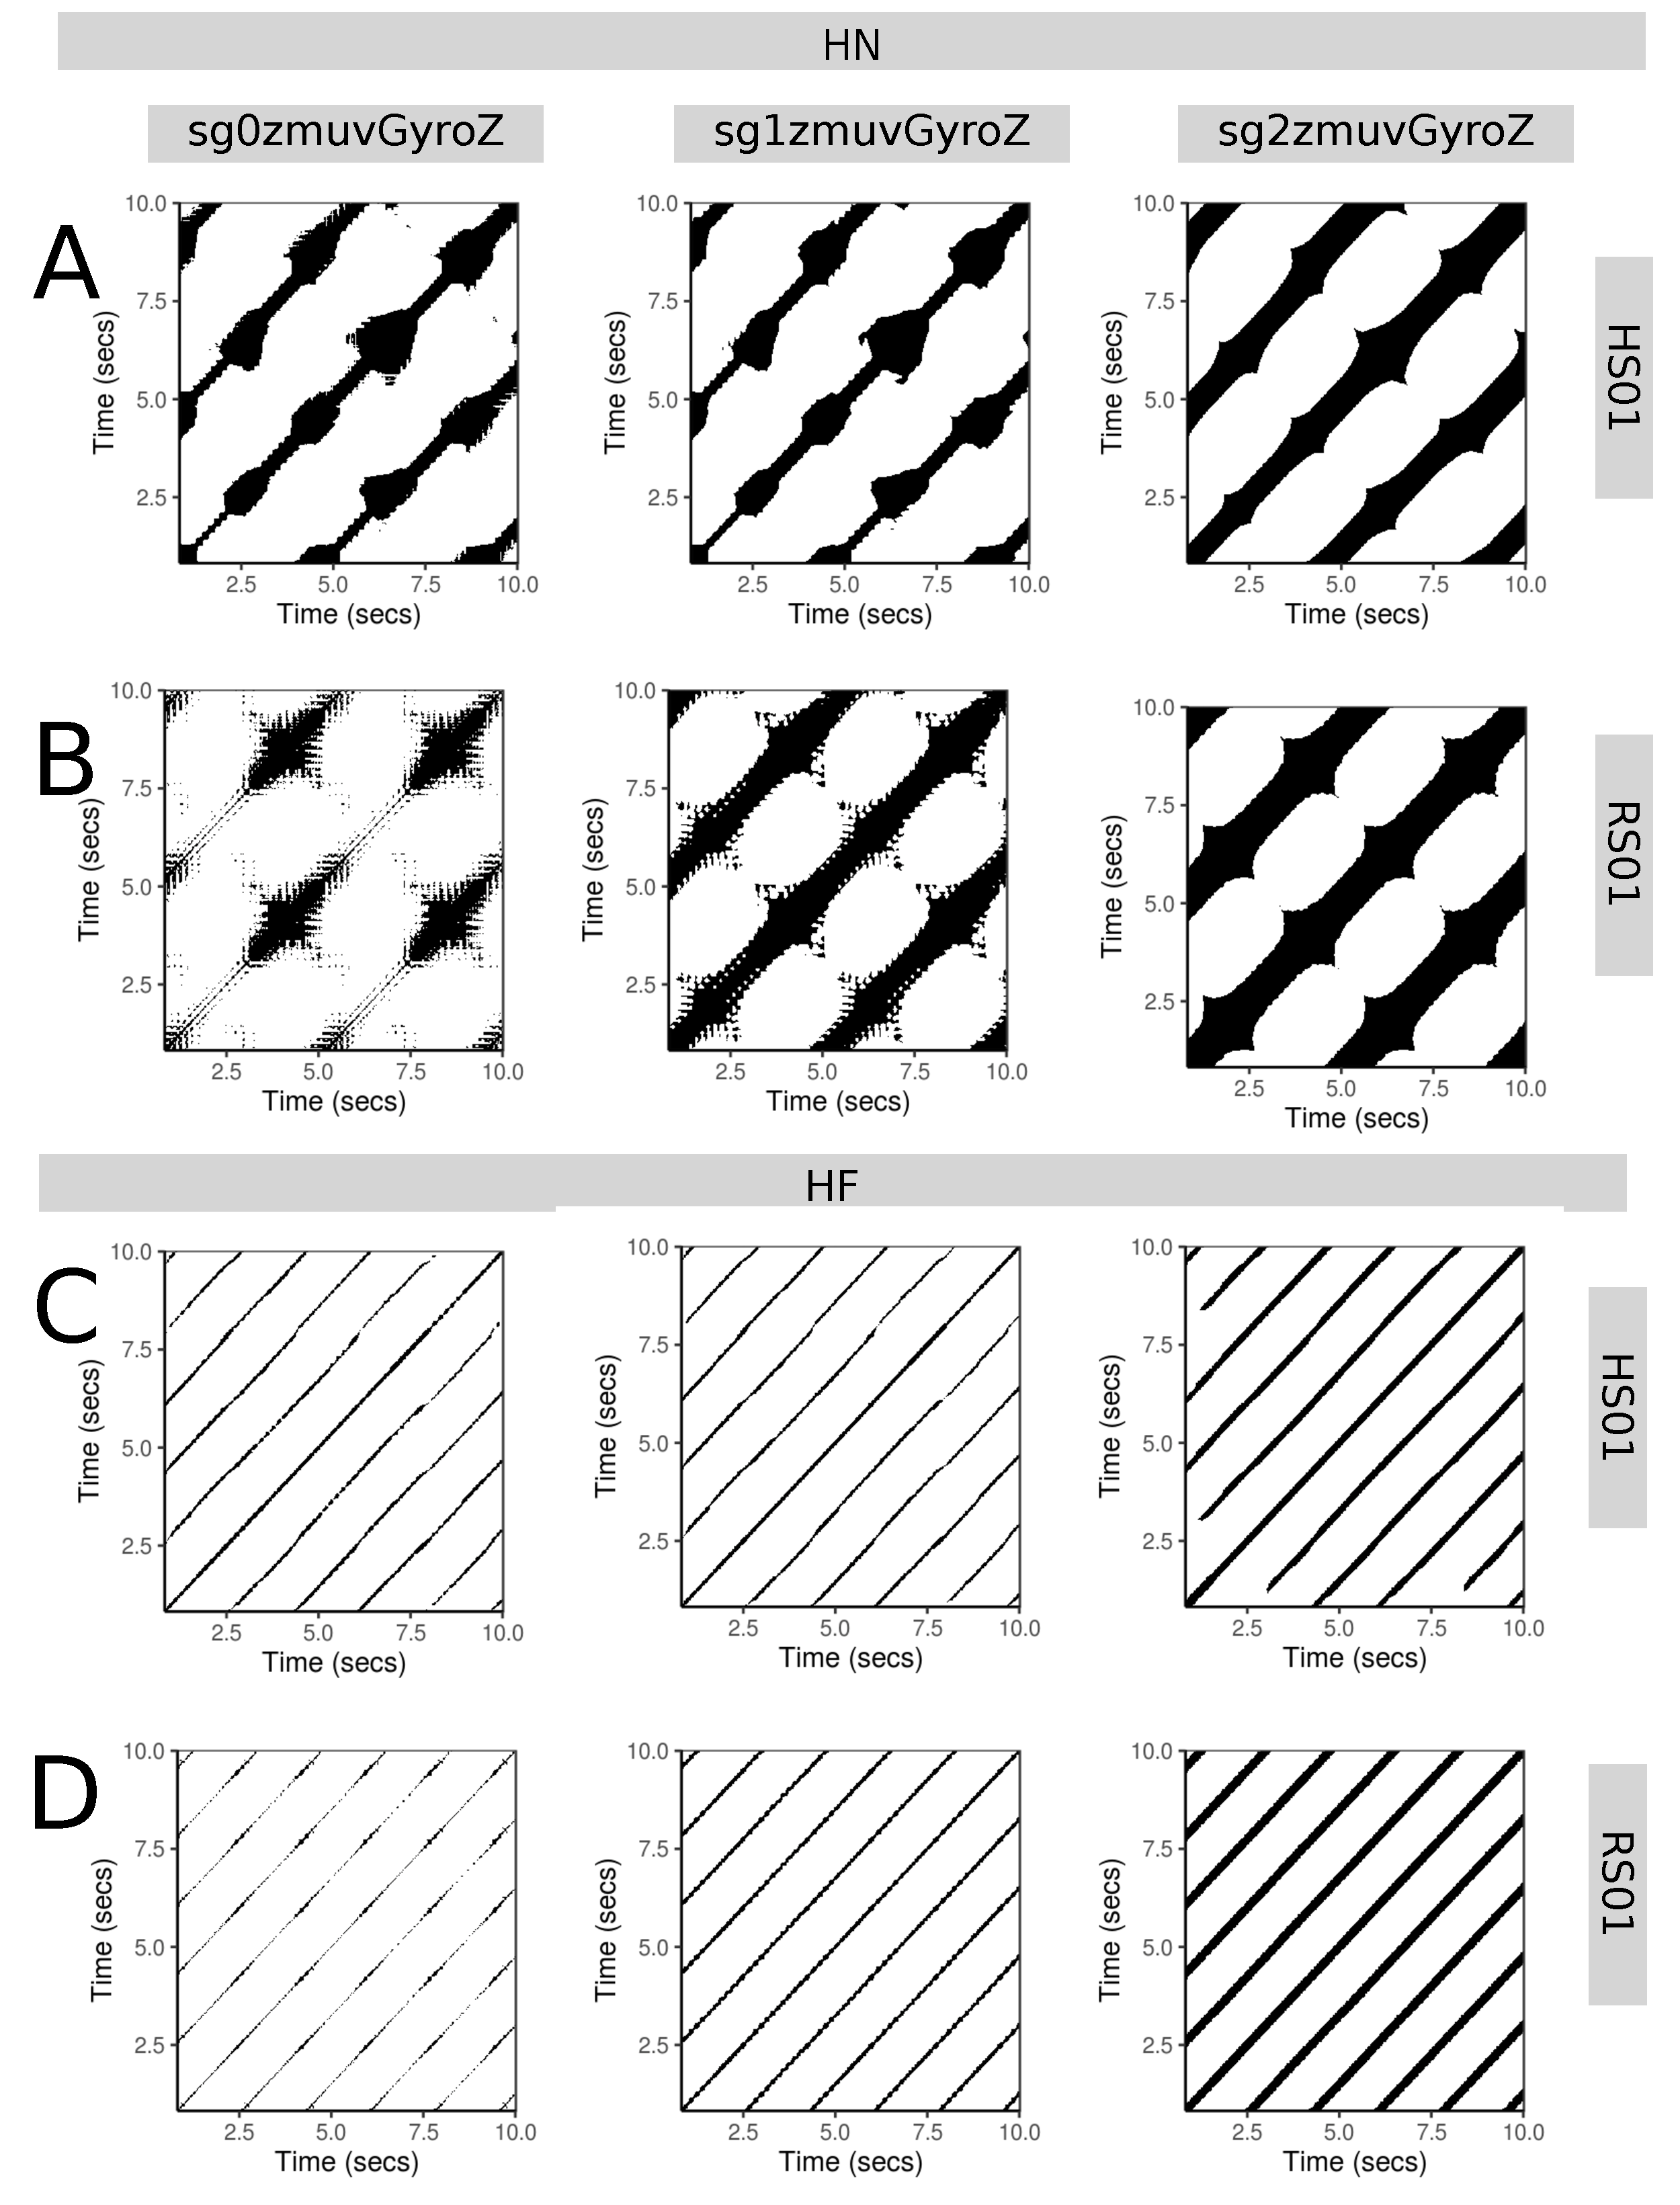
\includegraphics[width=1.0\textwidth]{figures/rps/pdf/rp_aH}
\caption{
	{\bf RPs for horizontal arm movements.}	
	Recurrence plots were computed with 
	embedding parameters $m=6$, $\tau=8$ and $\epsilon=1$.
	Code and data to reproduce the figure is available from \cite{srep2019}.
        }
    \label{fig:rp_aH}
\end{figure}
%%---------------------------------(FIGURE)------------------------------------
%%---------------------------------(FIGURE)-------------------------------------
\begin{figure}[ht]
\centering
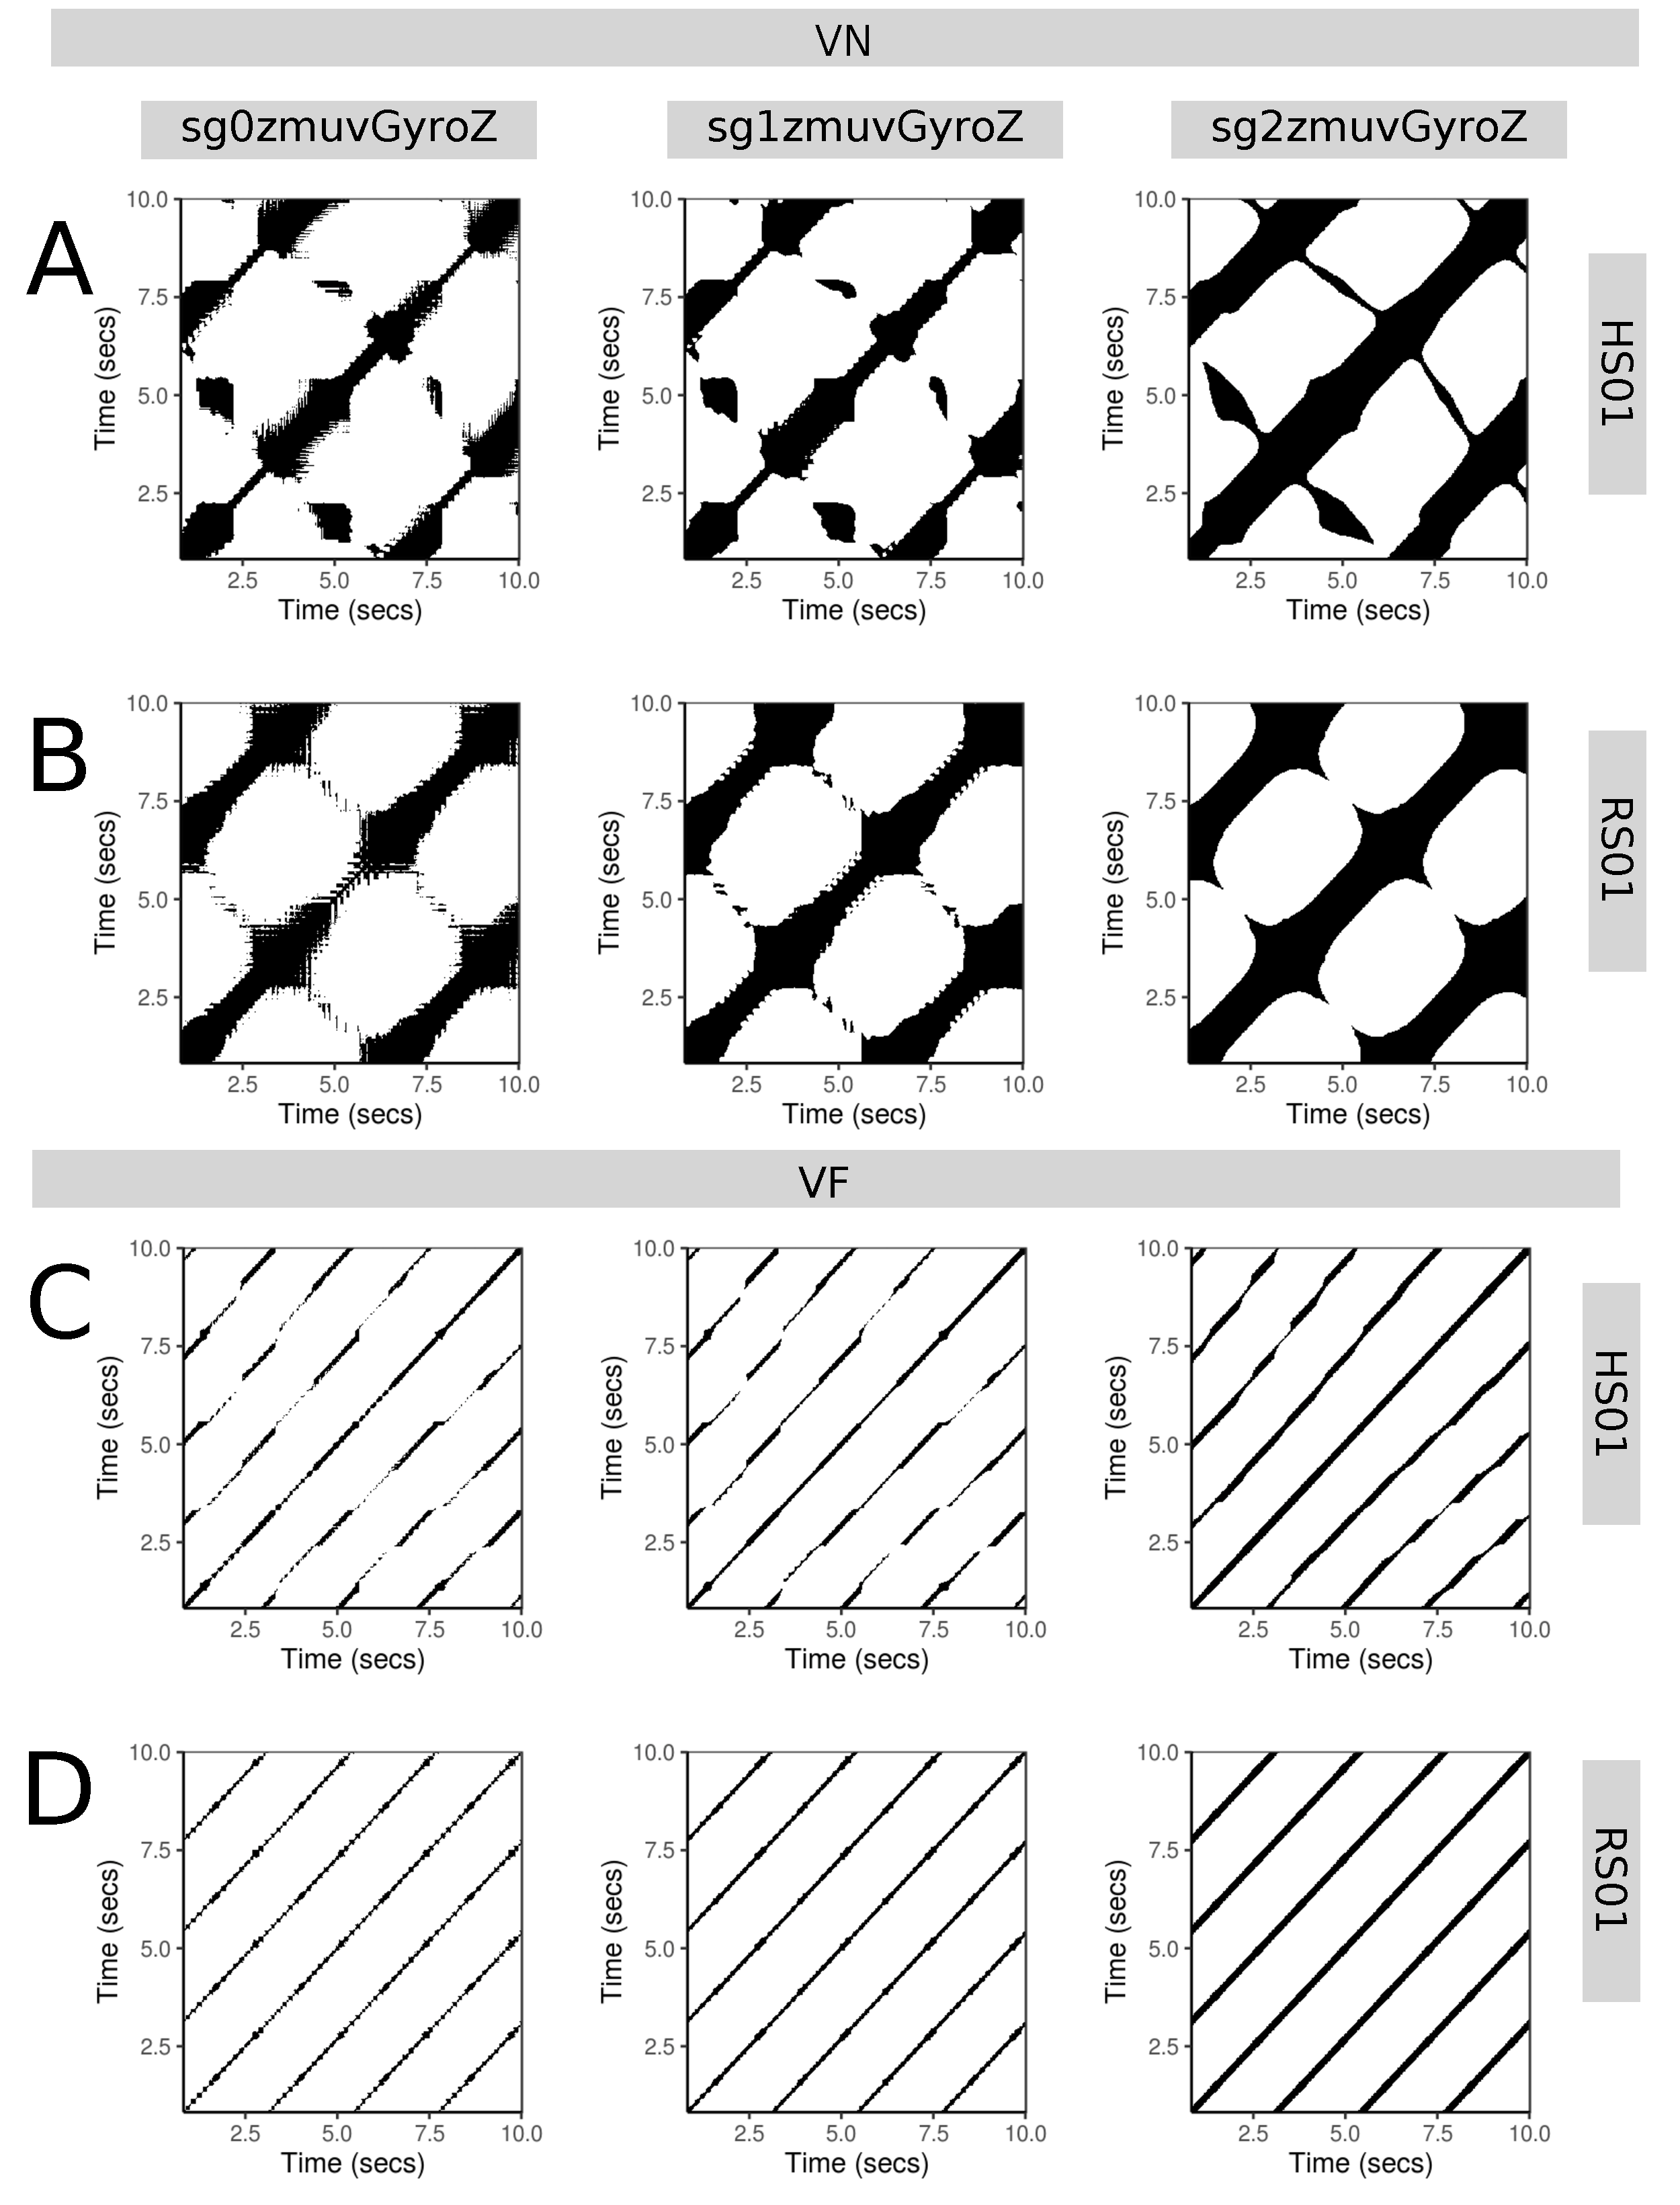
\includegraphics[width=1.0\textwidth]{figures/rps/pdf/rp_aV}
\caption{
	{\bf RPs for vertical arm movements.}	
	Recurrence plots were computed with 
	embedding parameters $m=6$, $\tau=8$ and $\epsilon=1$.
	Code and data to reproduce the figure is available from \cite{srep2019}.
        }
    \label{fig:rp_aV}
\end{figure}
%%---------------------------------(FIGURE)------------------------------------






\subsection*{Recurrence Quantification Analysis} \label{ch6:rqas}
%Considering the RPs for 20 participants performing four activities 
%(HN, HF, VN and VF) with sensors attached to the human and 
%to the humanoid robot (HS01, RS01) and the increase of smoothness 
%of time series (sg0zmuvGyroZ, sg1zmuvGyroZ and sg2zmuvGyroZ),
Similarly to RP, we computed four RQA metrics (REC, DET, RATIO and ENTR) 
with embedding parameters $m=6$, $\tau=8$ and 
recurrence threshold $\epsilon=1$.
 

\subsubsection*{REC values}
It can be seen in the box plots of Figs~\ref{fig:RQABP}(A) that REC values, 
representing the \% of black dots in the RPs, 
are more spread for HN and VN movements (higher interquartile range) 
than HF and VF movements (lower interquartile range) for HS01 sensor. 
In contrast, REC values for RS01 sensor present little variation 
(interquartile range of 0.01).
With regard to the increase of smoothness of time series 
(sg0, sg1 and sg2), REC values present little 
variation as the smoothness is increasing for time series from HS01 
(changes of mean values (rhombus)) while REC values are more affected with 
the smoothness for data from RS01 
(see the incremental changes of mean values (rhombus)).
%See Figs~\ref{fig:rec_aH} and \ref{fig:rec_aV} in appendix \ref{appendix:e:ep} 
%for more details about individual REC values for each participant.


\subsubsection*{DET values}
Figs \ref{fig:RQABP}(B) illustrate DET values, 
representing predictability and organisation of the RPs, 
which change very little (interquartile range is around 0.1) 
for type of movement, level of smoothness or type of sensor.
There is also increase of DET values as the smoothness of the signal increase 
(see the incremental changes of mean values (rhombus)).
It can be noted that the interquartile range for faster movements
(HF and VF) with no smoothing (sg0) is lower than the other
levels of smoothness (sg1 and sg2).
%See Figs~\ref{fig:det_aH} and \ref{fig:det_aV} in appendix \ref{appendix:e:ep} 
%for more details about individual DET values for each participant.

\subsubsection*{RATIO values}
Figs \ref{fig:RQABP}(C) present RATIO values, representing dynamic transitions, 
for horizontal and vertical movements.
It can be seen that RATIO values for HS01 sensor vary less 
for HN movements (interquartile range around 2)
than HF movements (interquartile range around 5).
%which is a similar behaviour of RATIO values for oRS01 sensor.
For faster movements (HF and VF), it can be noted a decrease of 
RATIO values as the smoothness of the time series is increasing (rhombus).
For normal movements (HN and VN), the decrease of RATIO values
is less evident than faster movements (see rhombus).
%See Figs~\ref{fig:ratio_aH} and \ref{fig:ratio_aV} in appendix 
%\ref{appendix:e:ep} 
%for more details about individual RATIO values for each participant.


\subsubsection*{ENTR values}
Figs \ref{fig:RQABP}(D) show ENTR values, Shannon entropy values 
which represent the complexity of 
the structure the time series, 
for type of movement, level of smoothness or type of sensor.
ENTR values for HS01 sensor show a higher variation  
(interquartile range around 0.5)
than ENTR values for RS01 sensor which appear 
to be more constant (interquartile range 0.1).
It can also be noted the increase of smoothness of time series 
also is presented with an increase of ENTR values (see gray rhombus).
%See Figs~\ref{fig:entr_aH} and \ref{fig:entr_aV} in appendix
%\ref{appendix:e:ep}
%for more details about individual ENTR values for each participant.


%%---------------------------------(FIGURE)-------------------------------------
\begin{figure}
\centering
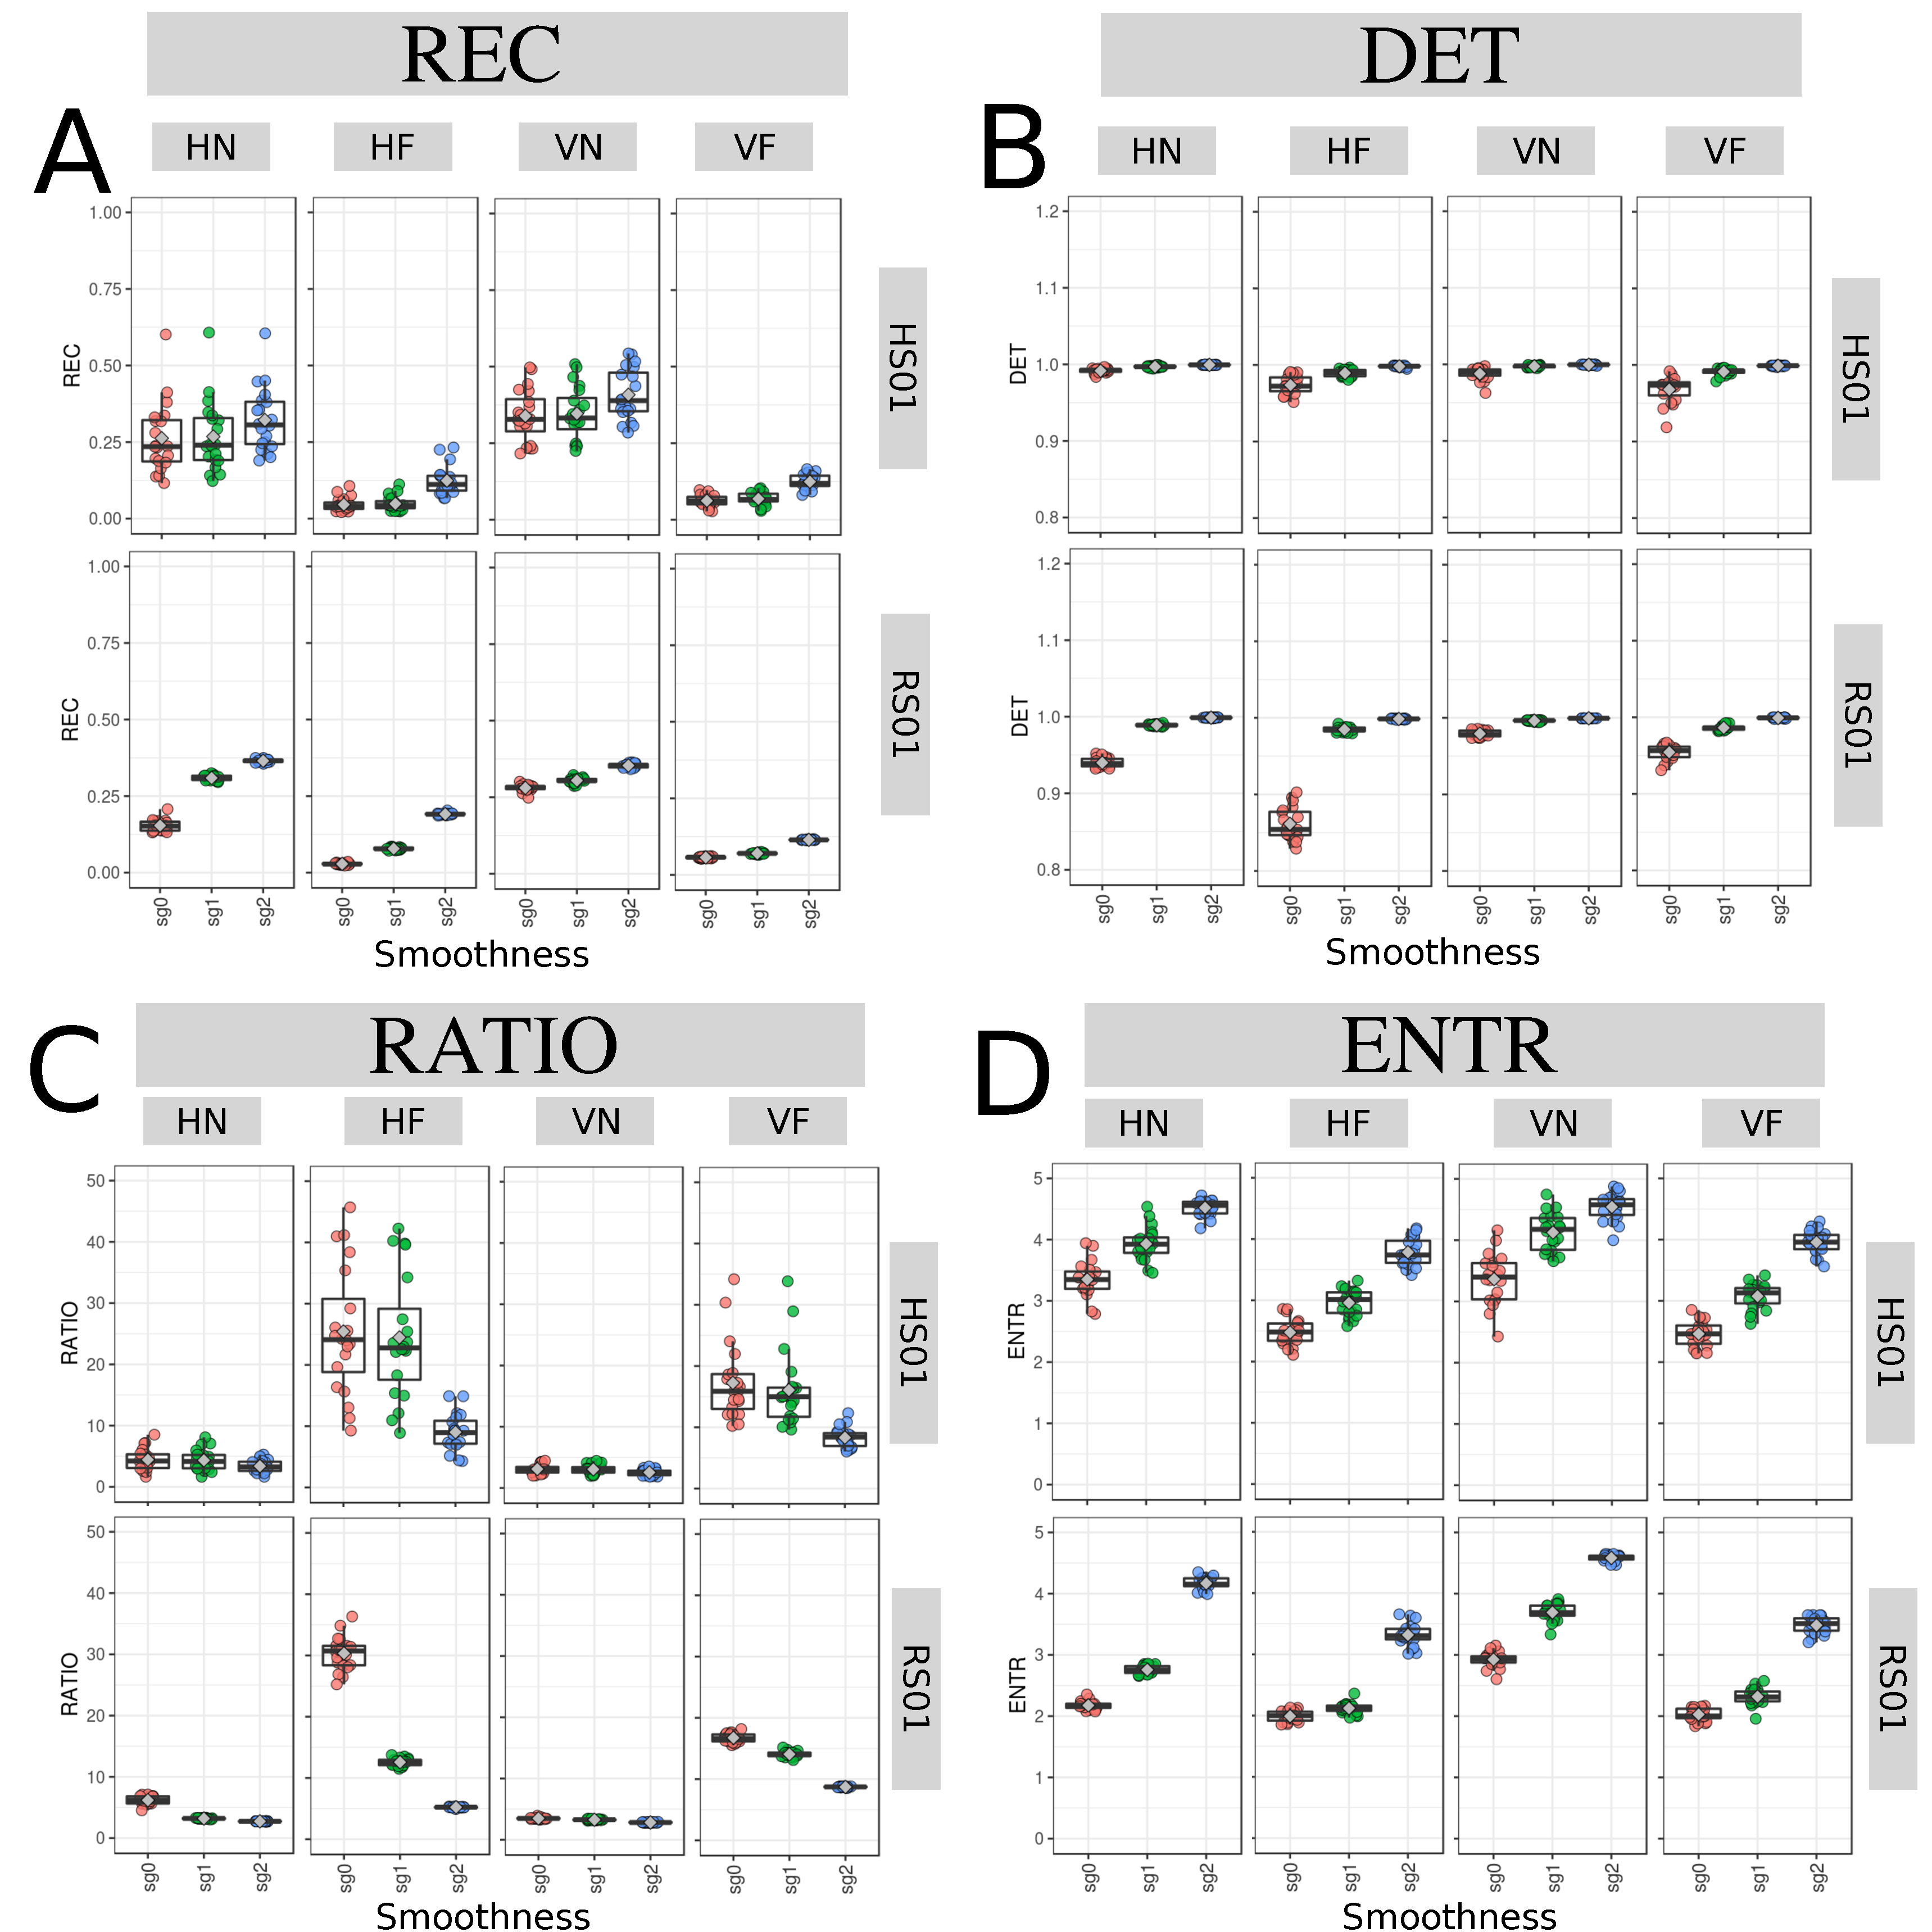
\includegraphics[width=1.0\textwidth]{figures/rqa/pdf/rqa-bp}
    \caption
	[Box plots for RQA values]{
	{\bf Box plots for RQA values.}
	Box plots of (A) REC, (B) DET, (C) RATIO, and (D) ENTR values 
	for 20 participants performing HN, HF, VN and VF movements
	with sensors HS01, RS01 and three smoothed-normalised  
	time series (sg0, sg1 and sg2).
	RQA values were computed with 
	embedding parameters $m=6$, $\tau=8$ and $\epsilon=1$.
	Code and data to reproduce the figure is available from \cite{srep2019}.
        }
    \label{fig:RQABP}
\end{figure}
%%---------------------------------(FIGURE)------------------------------------


\subsection*{3D RQA ENTR}
Choosing an appropriate recurrence threshold is crucial to get 
meaningful representations in RP and RQA, however, as previously shown, 
one can selected the default recurrence threshold of $\epsilon=1$, 
as long as it is able to represent the dynamical transitions 
in each of the time series \cite{marwan2011}. %%Marwan et al. \cite{marwan2011} 
However, to show how that the selection of recurrence threshold affects RQA
values, 
we computed ENTR values of RQA metrics for different embedding parameters
$[1,10]= \{ m \in \mathbb{R} | 1 \le m \le 10  \} $,
$[1,10]= \{ \tau \in \mathbb{R} | 1 \le \tau \le 10  \} $
with an increase of 1
and different recurrence thresholds 
$[0.2,3]= \{ \epsilon \in \mathbb{R} | 0.2 \le \epsilon \le 3.0  \} $
with increments of 0.1.
For easily visualisation, Figs \ref{fig:RQA-IND} only show 3D RQA for 
three recurrence thresholds $\epsilon=1, 2, 3$ with three levels of 
smoothness (sg0, sg1, sg2). It can be noted in Figs \ref{fig:RQA-IND} 
that the increase of recurrence threshold is associated to the increase 
of ENTR values in any of the levels of smoothness (see values of the ENTR bar).
One can also see that the maximum values of ENTR 
for $\epsilon=1$ and sg0 are for embedding dimensions of 2 
and then as $\epsilon$ increases the maximum values of ENTR are for
an associated increase of in the embedding dimension.
It can also be noted that the increase of level of smoothness (from sg0 to sg2) 
is associated with both the increase of ENTR values and its smoothed 3D shape.

%%---------------------------------(FIGURE)-------------------------------------
\begin{figure}
\centering
\includegraphics[width=1.0\textwidth]{figures/rqa/pdf/rqa_epsilons}
    \caption
	[3D RQA ENTR values]{
	{\bf 3D RQA ENTR values.}
	RQA ENTR values 
	for different embedding parameters
	$[1,10]= \{ m \in \mathbb{R} | 0 \le m \le 10  \} $,
	$[1,10]= \{ \tau \in \mathbb{R} | 0 \le \tau \le 10  \} $
	with an increase of 1
	and different recurrence thresholds $\epsilon=1, 2, 3$.
	RQA ENTR values are for $p03$, sensor HS01, of a window size of 10-secs (500 samples).
	Code and data to reproduce the figure is available from \cite{srep2019}.
        }
    \label{fig:RQA-IND}
\end{figure}
%%---------------------------------(FIGURE)------------------------------------



%of ENTR and plotted 3D surfaces using an unitary 
%and a decimal increase of 0.1 for recurrence thresholds 
% (Fig.~\ref{fig:topo_rqas}). 
%Hence, Fig.~\ref{fig:topo_rqas}(A) shows an increase for 
%REC values, the percentage of black docs in the RP, 
%as the recurrence threshold increase,
%while the variation for embedding parameters creates little decrease 
%of REC values as the embedding dimensions.
% increase and even a more slighter 
%decrements of REC values for the increase of $\tau$.
%For the 3D surface of DET values (Fig.~\ref{fig:topo_rqas}(B)), 
%representing 
%predictability and organisation of the RPs, one can be noted a plateau
%for DET values near to 1 for embedding dimension parameters of less 
%than 5 and recurrence threshold values of greater than 2 (red surface). 
%It can also be observed that the increases of delay embedding made 
%the DET values increase so as to make an cascade effect in the surface 
%along with the increase of dimension embedding $m$.
%For RATIO values, representing dynamic transitions, 
%Fig.~\ref{fig:topo_rqas} shows that the 3D surface present 
%a plateau (blue surface) of RATIO values 
%near to zero for recurrence thresholds greater than 1.0, while 
%fluctuations are more evident for recurrence thresholds of less than 1.0,
%particularly it can also be noted an increase in the fluctuations of 
%RATIO values as the embedding dimension is increasing. 
%For ENTR values in Fig.~\ref{fig:topo_rqas}(D), 
%representing the complexity of the structures in time series, 
%one can be noted that the increase of recurrence threshold is, 
%not strictly proportional to the increase of ENTR values. 
%It can also be observed in Fig.~\ref{fig:topo_rqas}(D)
%that the increase of delay embeddings affects 
%little the ENTR values for embedding dimensions of 1, while 
%for higher values of embedding dimensions 
%there is a decrease of ENTR values, and 
%there is a decrease of ENTR values as delay dimension value is increasing.
%%---------------------------------(FIGURE)-------------------------------------
%\begin{figure}
%\centering
%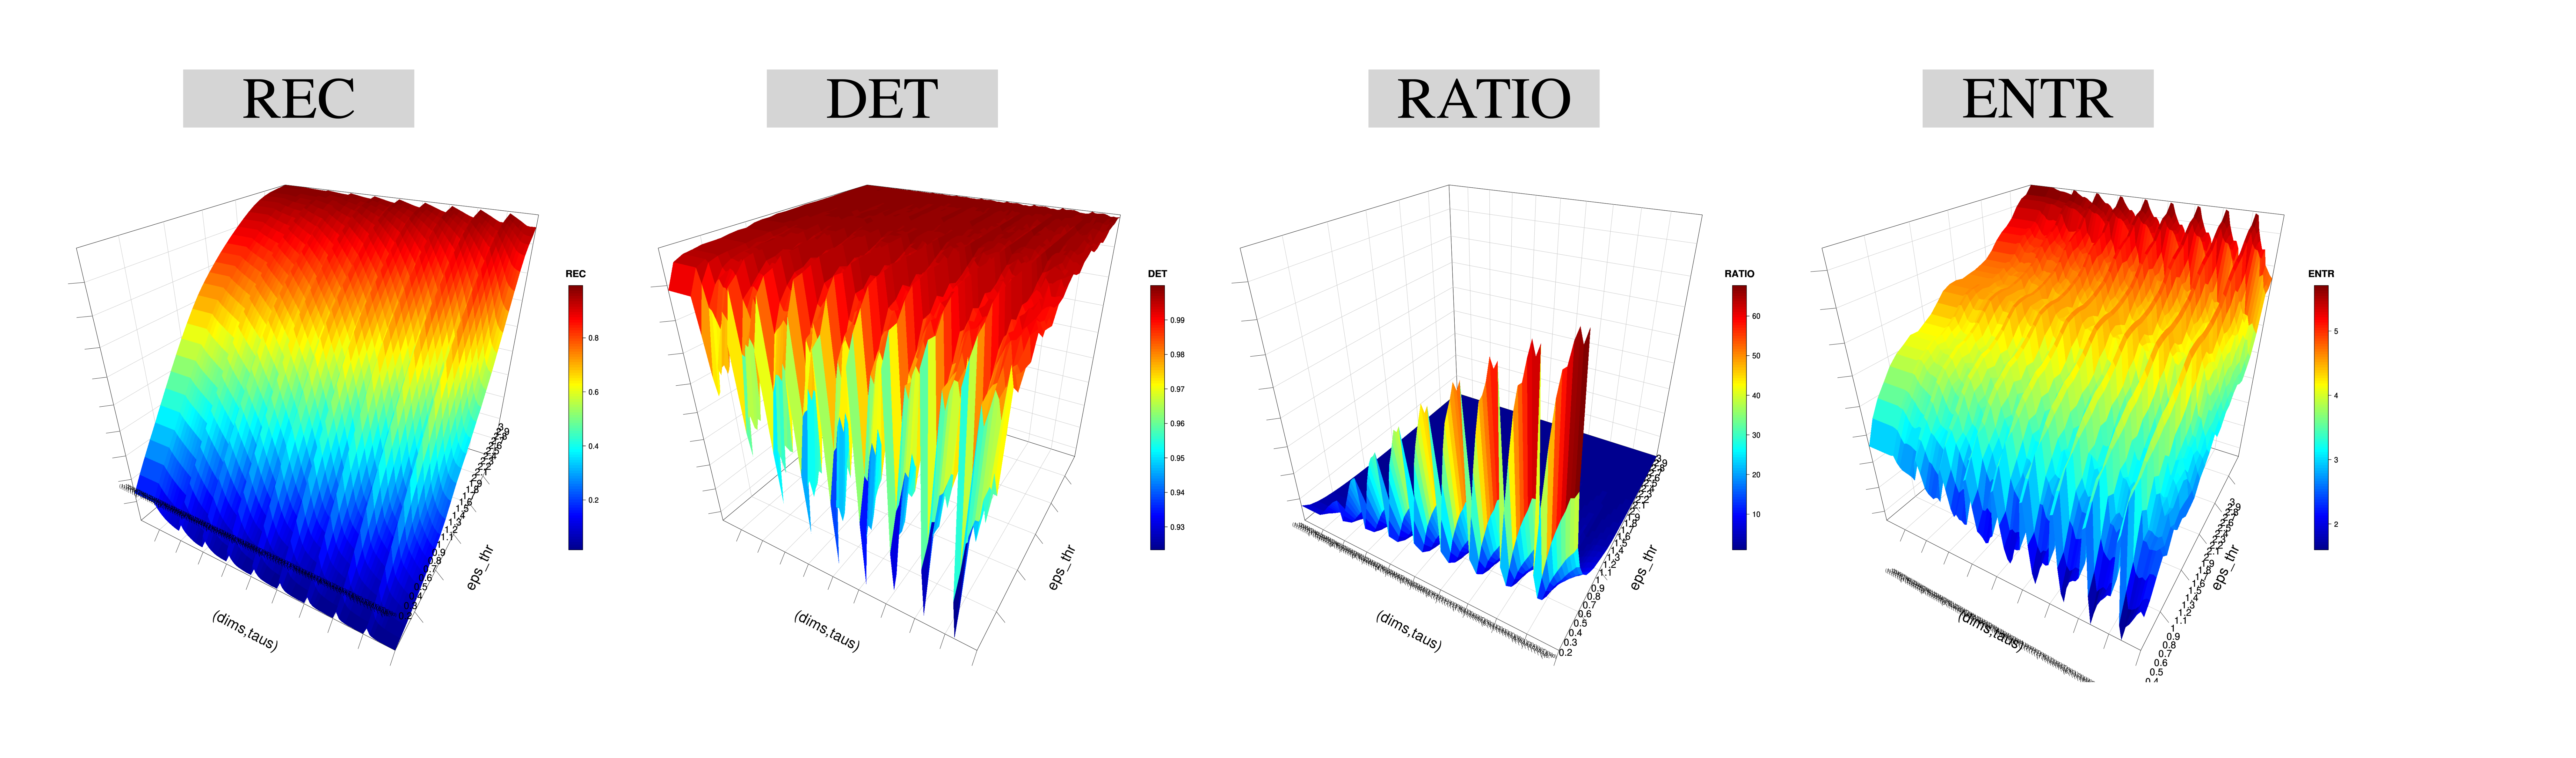
\includegraphics[width=1.0\textwidth]{rqas}
%    \caption
%	[3D surfaces for RQA metrics]{
%	{\bf 3D surfaces for RQA metrics.}
%	3D surfaces for (A) REC, (B) DET, (C) RATIO and (D) ENTR values 
%	with increasing pair of embedding parameters 
%	($0 \ge m \le 10$, $0 \ge \tau \le 10$) 
%	and recurrence thresholds (  $ 0.2 \ge \epsilon \le 3 $).
%	RQA metrics are computed with the time series of participant $p01$ using 
%	HS01 sensor, HN activity, sg0zmuvGyroZ axis and 500 samples 
%	for window size length.
%	Code and data to reproduce the figure is available from \cite{srep2019}.
%	}
%\label{fig:topo_rqas}
%\end{figure}
%%---------------------------------(FIGURE)------------------------------------
%




\subsection*{Other effects on 3D RQA ENTR values}

%Zbilut et al. \cite{zbilut1992} established RQA metrics with the aim of 
%determining embedding parameters, their method consisted on creating 3D 
%surfaces with RQA metrics with an increase of embedding parameters 
%($m$ and $\tau$), then Zbilut et al. \cite{zbilut1992} explored 
%fluctuations and gradual changes in the 3D surfaces that provide information 
%about the embeddings. Much recently, Marwan et al. \cite{marwan2015} 
%created 3D surfaces for visual selection of not only embedding parameters 
%but also recurrence thresholds. Following same methodologies, we explored 
%the stability and robustness of RQA metrics (REC, DET, RATIO and ENTR)
%using 3D surfaces by an unitary increase of the pair embedding 
%parameters ($0 \ge m \le 10$, $0 \ge \tau \le 10$) and a decimal increase 
%of 0.1 for recurrence thresholds ($ 0.2 \ge \epsilon \le 3 $) 
%(Fig.~\ref{fig:topo_rqas}). 
We also computed 3D surfaces of RQA metrics for different sensors 
and different activities (Fig~\ref{fig:3dRQAENTR_sensoractivities}).
From the maximum values of ENTR (lateral bars), one can see 
a decrease of ENTR values for activities going from normal to 
faster velocity and from human sensor (HS01) to robot sensor (RS01) 
(See Fig~\ref{fig:3dRQAENTR_sensoractivities}). 
%%---------------------------------(FIGURE)-------------------------------------
\begin{figure}[ht]
\centering
\includegraphics[width=1.0\textwidth]{figures/rqa/pdf/rqa_sensors_activities}
    \caption{
	{\bf 3D surfaces of RQA ENTR metrics for sensors and activities.}
	RQA ENTR values with embedding parameters
	$[1,10]= \{ m \in \mathbb{R} | 0 \le m \le 10  \}$,
	$[1,10]= \{ \tau \in \mathbb{R} | 0 \le \tau \le 10  \}$
	for different activities and sensors. 
	RQA ENTR values are for $p03$, sg0 and window size of 10-secs (500 samples).
	Code and data to reproduce the figure is available from \cite{srep2019}.
       }
\label{fig:3dRQAENTR_sensoractivities}
\end{figure}
%%---------------------------------(FIGURE)-------------------------------------


%RQA metrics are also affected by 
%the window length where for example four window lengths of 100, 250, 500 
%and 750 samples (Fig.~\ref{fig:topo_sensoractivities}). 

%Similarly, 3D surfaces of RQA metrics were also computed for three 
%participants (Fig.~\ref{fig:topo_participants}).

%X Three level of 
%X smoothness were computed for RQA metrics showing smoothed 3D surfaces and 
%X the level of smoothness increase (Fig.~\ref{fig:topo_smoothness}).



%*******************************************************************************
%*******************************************************************************
%*******************************************************************************
\section*{Discussion}
%The Discussion should be succinct and must not contain subheadings.


%DISCUSSION
%Similarly as with the Reconstructed State Spaces, 
%the differences in the RPs can be easily noticed by eye 
%for different time series (Figs~\ref{fig:rp_aV} and ~\ref{fig:rp_aH}), 
%which lead us to apply Recurrence Quantification Analysis (RQA) 
%in order to have an objective quantification of each of the time series.
%That said, 
%%Considering the time series of Fig~\ref{fig:ts}, 
%


It is evident that time series from different sources 
(participants, movements, axis type, window length or levels of smoothness) 
presents visual differences for embedding parameters and therefore for RRSs. 
For which, the selection of embedding parameters was our first challenge 
where we computed embedding parameters for each time series 
(Fig \label{fig:caoami}) and then computed a sample mean over 
all time series in order to get two embedding parameters 
to compute all RRSs (Figs \label{fig:rss_aHw10} and \label{fig:rss_aVw10}). 
%with its corresponded type of movement. 
Then we found that the quantification of variability with regard to 
the shape of the trajectories in RSSs requires more investigation 
since our original proposed method base on euclidean metric failed 
to quantify those trajectories. Specially, for trajectories which 
were not well unfolded. 
With that in mind, we apply 
Recurrence Quantification Analysis (RQA) metrics 
(REC, DET, RATIO and ENTR) in order to avoid any subjective interpretations 
or personal bias with regard to the representation of the trajectories in RSSs.


\subsection*{RQA metrics with fixed parameters}
Considering that RQA metrics were computed with fixed embedding parameters 
($m=6$ and $\tau=8$) and recurrence thresholds ($\epsilon=1$), we found 
the following. REC values, which represents the \% of black points in the RPs, 
were more affected with and increase in normal speed movements (HN and VN) 
than faster movements (HF and VF) for the sensor attached to the participants 
(HS01). Such decrease of REC values from normal speed to faster speed 
movements is also presented in data from sensor attached to the robot (RS01), 
and little can be said with regard to the dynamics of the time series coming 
from RS01 (Fig \ref{fig:RQABP}A).
Similarly, DET values, representing predictability and 
organisation in the RPs, present little variation in the any of the time 
series where little can be said (Fig \ref{fig:RQABP}B).
In contrast, RATIO values, which represent 
dynamic transitions, were more variable for faster movements (HF and VF) 
than normal speed movements (HN and VN) with sensors attached to the 
participants (HS01). For data coming from sensors attached to the robot 
(RS01), RATIO values from horizontal movements (HN, HF) appear to vary 
more than values coming from vertical movmentes (VN, VF) 
(Fig \ref{fig:RQABP}C).
With that, it can be said that RATIO values can represent a bit better
than REC or DET metrics for the variability of imitation activities in 
each of the conditions for time series.
Similarly, ENTR values for HN were higher than values for HF
and ENTR values varied more for sensor attached to participants 
than ENTR values for sensors of the robot. It is evidently that 
the higher the entropy the more complex the dynamics are, 
however, ENTR values for HN appear a bit higher than HF values, 
for which we believe this happens because of the structure the time series
which appear more complex for HN than  HF movements which presented a 
more consistence repetition (Fig \ref{fig:RQABP}D).


Additionally, we observed that some RQA metrics are affected by the 
smoothness of data. 
%For which, we also explored the effect of smoothness of raw-normalised data 
%where, 
For instance, REC and DET values were not completely affected by the 
smoothness of time-series since these RQA values seemed to be constants. 
However, for RATIO values, 
the effect of smoothness can be noticed with a slight decrease of amplitude 
in any of the time series conditions which is also presented with ENTR values.


\subsection*{RQA metrics with different parameters}
Iwansky et al. \cite{iwanski1998} stated that patterns in RPs and 
metrics for RQA are independent of embedding dimension parameters, 
however, that is not the case when using 
different recurrence thresholds. Such changes of recurrence threshold values 
can modify the patterns in RPs and therefore the values of RQA metrics.
We therefore computed 3D surfaces to explore the sensibility and robustness of 
embedding parameters and recurrence threshold in RQA  metrics. Following the 
same methodology of computing 3D surfaces, we also considered variation of 
window length size to present RQA metrics dependencies with embedding 
parameters, recurrence thresholds and window length size.



\section*{Conclusions}
Generally, we can conclude that using a different level of 
smoothness for time series help us to visualise and to quantify 
the variation of movements 
between participants using RSSs, RPs and RQA. 
It is important to mention that some RQA's metrics 
(e.g. DET and ENTR) are more robust to the effect of 
smoothness of time series.
However, using determined RQA metrics will be depend on 
what one want to quantify, for instance, one can compute 
predicability, organisation,  
dynamics transitions, or complexity and determinism of the 
input time series. However, RQA metrics show certain constrains with 
regard to activity type, window length and structure of the time series.
%Similarly, such differences in time series created differences in each of the 
%RQA metrics, 
For instance, RATIO and ENTR are helpful to distinguish 
differences in any of the categories of the time series (sensor, activity, 
level of smoothness and number of participant), however for certain time series
such as time series from the sensor attached to the robot seemed to have 
little variations between each of the participants. 
The latter phenomena was in a way evidently as robot degrees of freedom 
did not allow it to move with a wide range of variability. 

Additionally, we can point out that even thought our experiment is 
limited to twenty healthy right-handed participants of a range age 
of mean 19.8 SD=1.39, RQA metrics show the potential to quantify 
human movement variability in the context of 
human-humanoid imitation activities.

%With that in mind, we conclude that 
%quantification of human-humanoid imitation activities is possible for 
%participants of different ages, state of health and anthropomorphic features.


%Such understanding and measurement of movement variability using
%cheap wearable inertial sensors lead us to have a more intuitive selection of parameters
%to reconstruct the state spaces and to create meaningful interpretations
%of the recurrence plots and the results of the metrics with recurrence quantification 
%analysis. 
%


%
%However, we believe that further investigation is required to find the 
%right balance between the level of smoothness of the signal
%and defining what is the aim of RQA where 
%its representations using RSS, RP and RQA.
%Specially, where the level of smoothness does not affect 
%the variation of each of the movements quantification. 
%%We can also conclude that finding the right balance between 
%%smoothness and the raw data to capture movement variability is 
%%a still a problem that has many avenues for exploration.
%



\section*{Future Work}

\subsection*{Inertial Sensors}
To have more fundamental understating of nature of signals collected through 
inertial sensors in the context of human-robot interaction, we are considering 
to apply derivates to the acceleration data. We can then explore the jerkiness 
of movements and therefore the nature of arm movements which typically have 
minimum jerk \cite{flash1985}, its relationship with different body 
parts \cite{devries1982, mori2012} or the application of higher derivatives 
of displacement with respect time such as snap, crackle and pop \cite{eager2016}.

\subsection*{RQA ENTR}
Having shown that RQA ENTR metrics are robust against different data
time series, we believe that further investigation is required to be done. 
For example, Marwan et al. \cite{marwan2007, marwan2015} reviewed 
different aspects to compute RPs using different criteria for neighbours, 
different norms ($L_{1-norm}$, $L_{2-norm}$, or $L_{\infty-norm}$ ) or 
different methods to select the recurrence threshold $\epsilon$, 
such as using certain percentage of the signal \cite{letellier2006}, 
the amount of noise or using a factor based on the standard deviation 
of the observational noise among many others \cite{marwan2007}.





%*******************************************************************************
%*******************************************************************************
%*******************************************************************************
\section*{Methods}
\subsection*{State Space Reconstruction}
The method of state space reconstruction was originally proposed by 
\cite{packard1980} and formalised by \cite{takens1981}. Since then, different 
investigations and disciplines have benefited from the use of the method of 
state space reconstruction \cite{aguirre2009, stergiou2011, frank2010, 
sama2013, Quintana-Duque2016}. The method of state space reconstruction is 
based on uniform time-delay embedding methodology which is a simple 
matrix implementation that can reconstruct an unknown $d-$dimensional 
manifold $M$ from a scalar time series (e.g. one-dimensional 
time series in $\mathbb{R}$). A manifold, in this context, is a 
multidimensional curved surface within a space (e.g. a saddle) 
\cite{guastello-gregson2011}.

The use of a scalar time series is the main advantage of the method of state 
space reconstruction which in essence preserve dynamic invariants such as 
correlation dimension, fractal dimension, Lyapunov exponents, Kolmogorov-Sinai 
entropy and detrended fluctuation analysis \cite{bradley2015, 
Quintana-Duque2012, Quintana-Duque2013, Quintana-Duque2016, krakovska2015}.
However, selecting appropriate embedding parameters which are sued to apply the 
state space reconstruction is still an open challenge for which we present 
introductions for the methodologies to compute such embedding parameters 
With that in mind, in the following subsections, we describe in more detail 
the state space reconstruction theorem (RSSs), uniform time-delay embedding 
theorem (UTDE), false nearest neighbours (FNN) and average mutual 
information (AMI). 
%and other methodologies for state space reconstruction.

\subsection*{State Space Reconstruction Theorem}
Following the notation employed in \cite{casdagli1991, garland2016, gibson1992,
uzal2011, uzal2010, takens1981}, state space reconstruction is defined by:
%%********************************[EQUATION]************************************
\begin{equation}\label{eq:ssr}
  s(t)=f^t [s(0)],
\end{equation}
%%********************************[EQUATION]************************************
where $s$, $s: A \rightarrow M$ given that $A \subseteq \mathbb{R}$ and 
$M \subseteq \mathbb{R}^d$, represents a trajectory which evolves in an 
unknown $d-$dimensional manifold $M$, $f: M \rightarrow M$ is an evolution 
function and $f^t$, with time evolution $t \in \mathbb{N}$, is the $t$-th 
iteration of $f$ that corresponds to an initial position 
$s(0) \in M $ \cite{takens1981}.
%$f$ is a smooth dynamical system, where smooth means a 
%continuously differentiable system
%(e.g. derivatives exist at all points) \cite{guastello-gregson2011}.
Then, a point of a one-dimensional time series $x(t)$ in $\mathbb{R}$, 
can be obtained with
%%********************************[EQUATION]************************************
\begin{equation}\label{eq:measurement}
  x(t)=h[s(t)],
\end{equation}
%%********************************[EQUATION]************************************
where $h$ is a function, $h: M \rightarrow \mathbb{R}$, defined on the trajectory $s(t)$.
Reconstructed state space can then be described as an $n-$dimensional state 
space defined by $y(t)=\Psi[\boldsymbol{X}(t)]$ where 
$\boldsymbol{X}(t) = \{ x(t), x(t-\tau) , ...,x(t - (m-1)\tau  ) \}$ 
is the uniform time-delay embedding with a dimension embedding $m$
and delay embedding $\tau$ and
$ \Psi: \mathbb{R}^m \rightarrow \mathbb{R}^n$ is a further transformation
of dimensionality (e.g. Principal Component Analysis, 
Singular Value Decomposition, etc) being $n \leq m$.
With that in mind, uniform time-delay embedding, $\boldsymbol{X}(t)$, 
defines a map $\Phi: M \rightarrow \mathbb{R}^m$ such that 
$\boldsymbol{X}(t) = \Phi(s(t))$,
where $\Phi$ is a diffeomorphic map \cite{takens1981}
whenever $\tau > 0$ and $m > 2d_{box}$ and $d_{box}$ is the box-counting
dimension of $M$ \cite{garland2016}.
% "Given two manifolds $M$ and $N$, a differientiable map $f: M \rightarrow N$
% is called diffeomorphic if it is one-to-one correspondence and its inverse
% $f^{-1}: N \rightarrow M$ is differientiable as well \cite{wiki:diffeomorphic}".
Then, if $\Phi$ is an embedding of evolving trajectories in the reconstructed 
space then a composition of functions represented with $F^t$ is induced on the
reconstructed state space determined:
%by true smooth dynamical system $f^t$ and $\Phi$:
%********************************[EQUATION]************************************
\begin{equation}\label{eq:st}
  \boldsymbol{X}(t)=F^t [\boldsymbol{X}(0)] = \Phi \circ f^t \circ \Phi ^{-1}[\boldsymbol{X}(0)].
\end{equation}
%%********************************[EQUATION]************************************
With this in mind, an embedding is defined as "a smooth one-to-one 
coordinate transformation with a smooth inverse" and the total reconstruction 
map is defined as $ \Xi = \Psi \circ \Phi $ \cite{casdagli1991}.
Fig~\ref{fig:ssr} illustrates the state space reconstruction.
%%---------------------------------(FIGURE)-------------------------------------
\begin{figure}[ht]
\centering
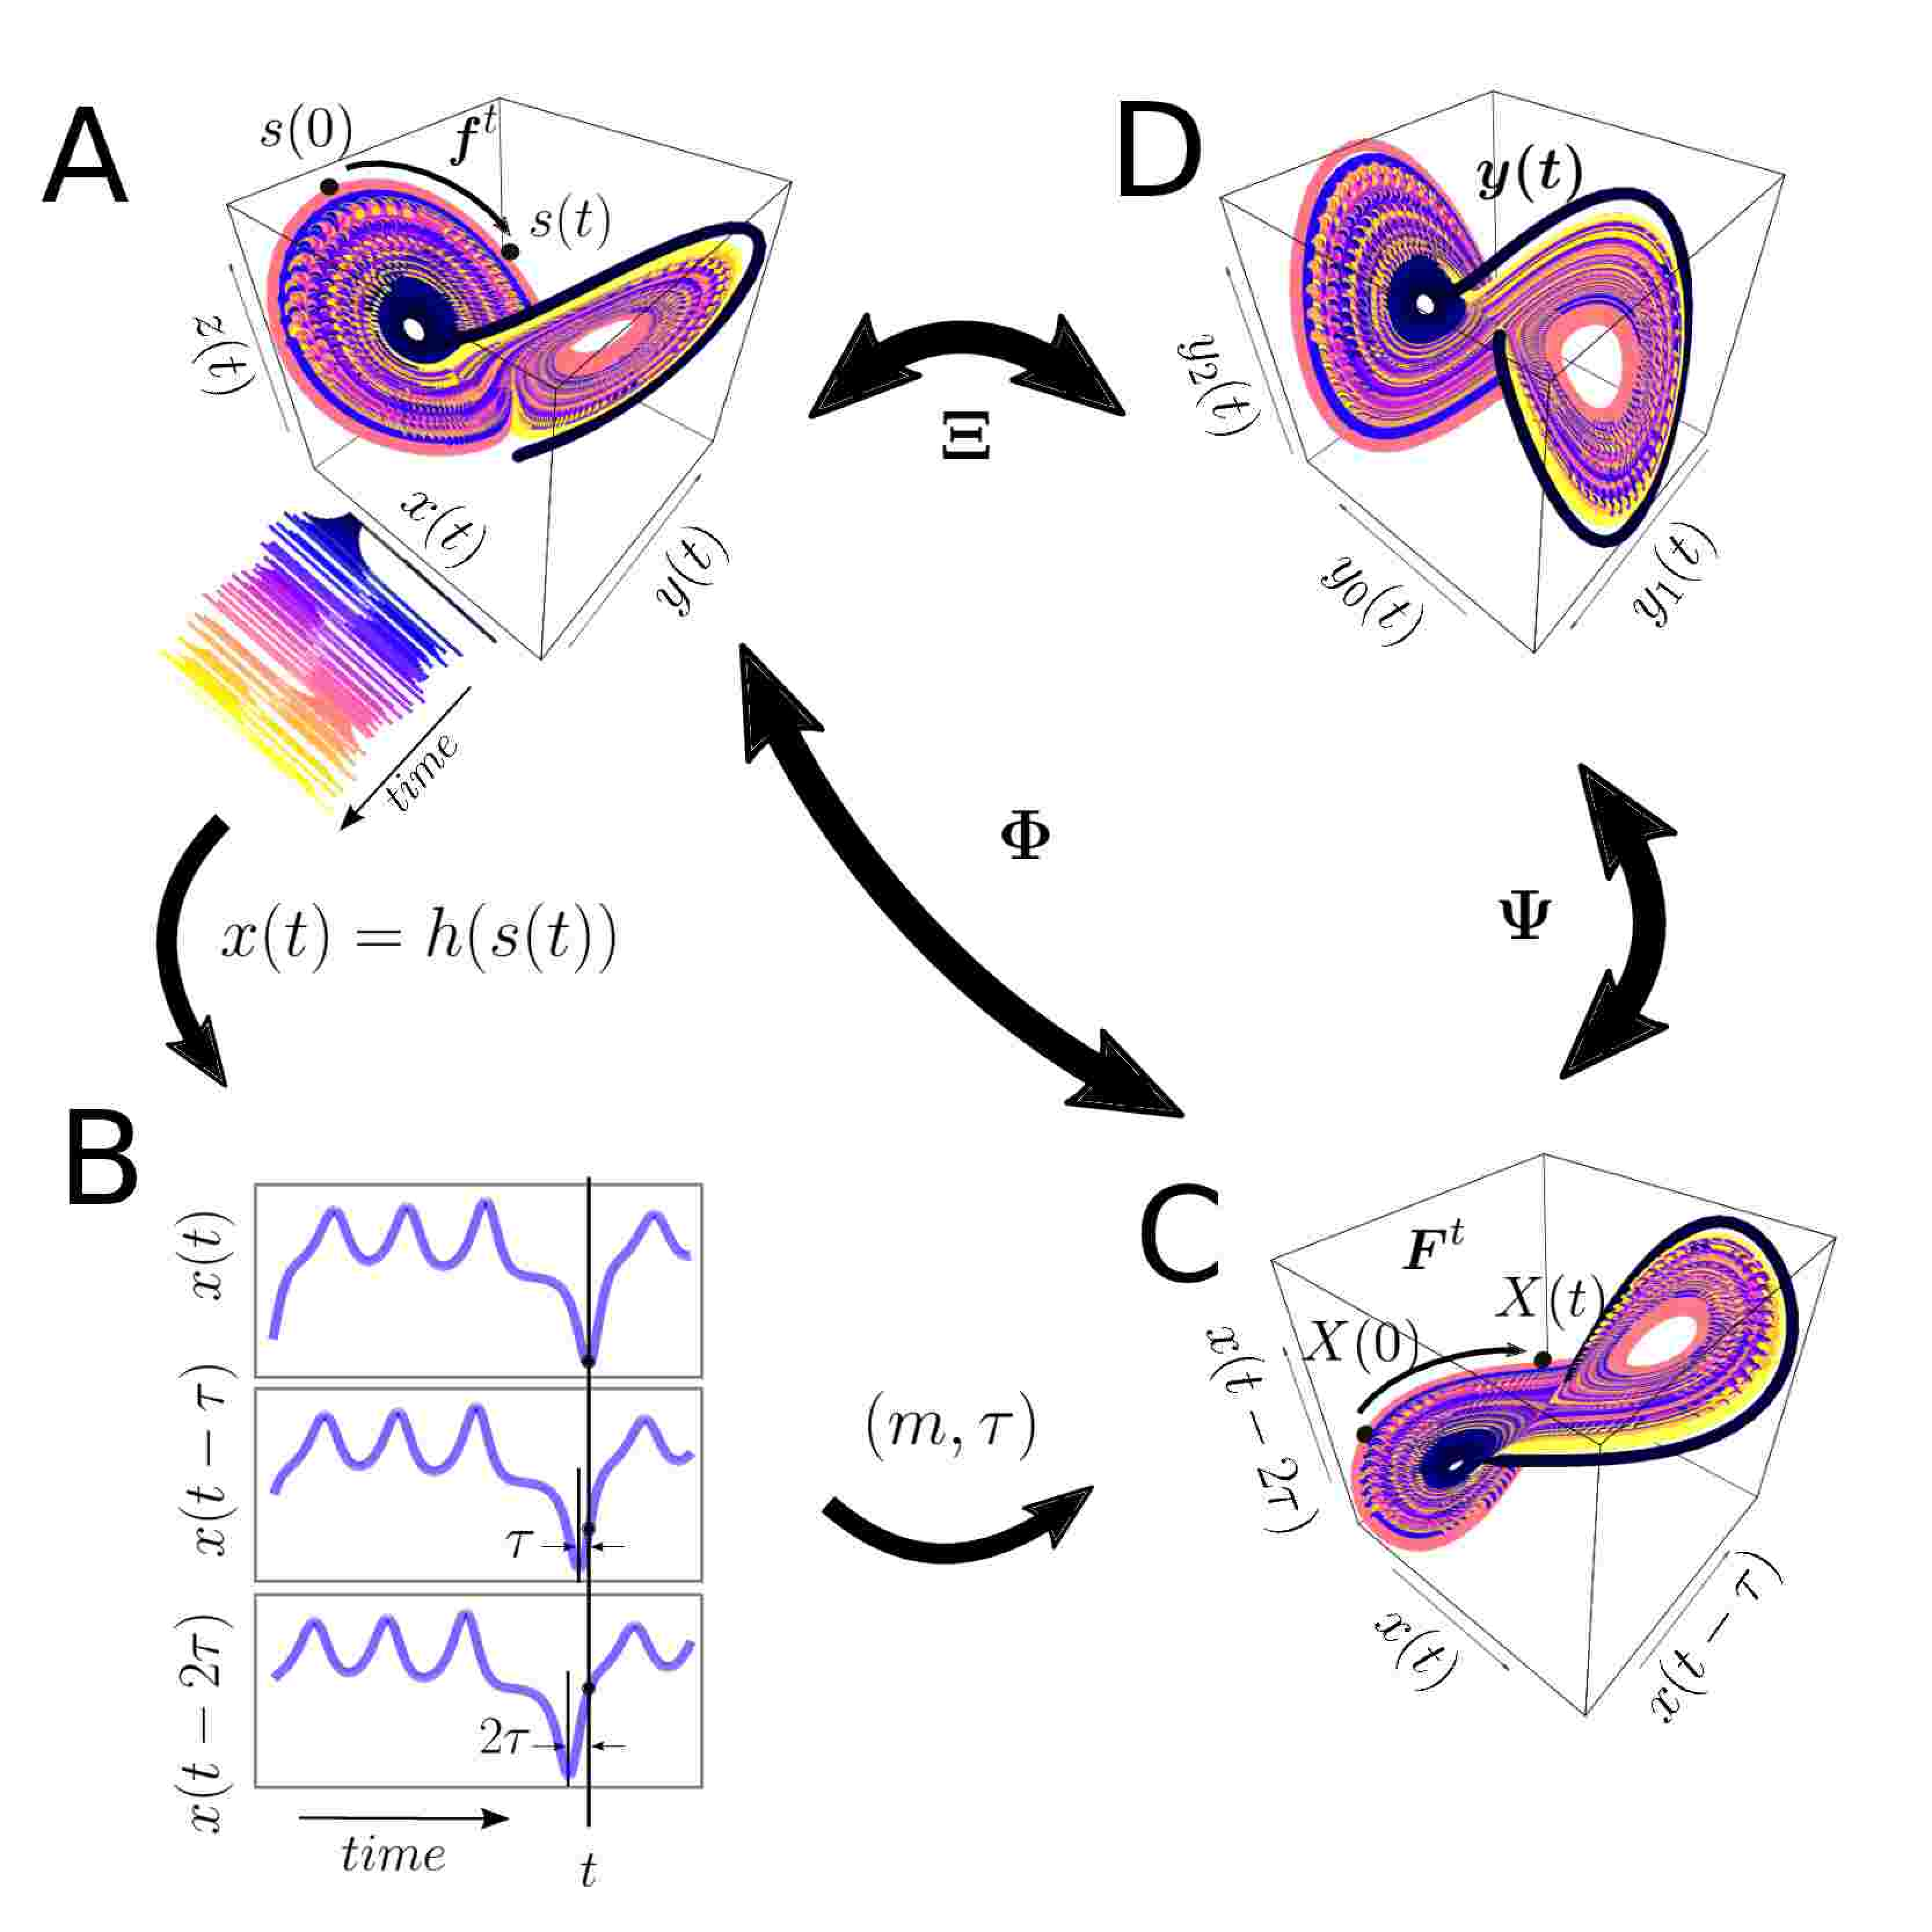
\includegraphics[width=1.0\textwidth]{figures/methods/rss/pdf/rss}
    \caption{
	{\bf State space reconstruction methodology.}
	State space reconstruction is based on $x(t)=h[s(t)]= h[f^t [s(0)]]$
	where $f^t$ is the true dynamical system, $s(t)$ indicates the state,
    	$s$, at time, $t$,  and $h[ ]$ the measurement function. 
    	The time-delay embedding represented as the $\Phi$, maps the original
    	$d-$dimensional state $s(t)$ into the $m-$dimensional uniform 
	time-delay embedding matrix $\boldsymbol{X}(t)$.
    	The transformation map $\Psi$ then maps $\boldsymbol{X}(t)$ into 
	a new state $y(t)$ of dimensions $n < m$.
    	(A) $M-$dimensional manifold representing the state space 
	(e.g. Lorenz system);
    	(B) Delayed copies of $1-$dimensional $x(t)$ from the Lorenz system;
   	(C) $m-$dimensional reconstructed state space with 
    	\texorpdfstring{$m$}{m} and    \texorpdfstring{$\tau$}{T}, and 
    	(D) $y(t)$ is the $n-$dimensional reconstructed state space.
	The total reconstruction map is represented as $\Xi = \Psi \circ \Phi $
	where $\Phi$ is the delay reconstruction map and 
	$\Psi$ is the coordinate transformation map.
	This figure is adapted from 
   	\cite{Quintana-Duque2012, casdagli1991, uzal2011}.
	Code and data to reproduce the figure is available from \cite{srep2019}.
    }
    \label{fig:ssr}
\end{figure}
%%---------------------------------(FIGURE)-------------------------------------



\subsection*{Uniform Time-Delay Embedding (UTDE)}\label{sec:utimedelayembedding}
Frank et al. and Sama et al. refer to the state space reconstruction
as "time-delay embeddings" or "delay coordinates" \cite{frank2010, sama2013}. 
However, we consider the term "uniform time-delay embedding"
as more descriptive and appropriate terminology for our work.
Hence, the uniform time-delay embedding is represented as a matrix of uniform delayed 
copies of the time series $\{ \boldsymbol{x}_n \}_{n=1}^N$ where $N$ is 
the sample length of $\{ \boldsymbol{x}_n \}$ and $n$ is index for the 
samples of $\{ \boldsymbol{x}_n \}$.
$\{ \boldsymbol{x}_n \}_{n=1}^N$ has a sample rate of $T$.
The delayed copies of $\{ \boldsymbol{x}_n \}$ are uniformly separated by $\tau$
and represented as $\{\boldsymbol{ \tilde{x} }_{n- i\tau} \}$
where $i$ goes from $0,1, \dots, (m-1)$.
Generally speaking, $\{\boldsymbol{ \tilde{x} }_{n- i\tau} \}$ contains
information of unobserved state variables and encapsulates the information of
the delayed copies of the available time series in the uniform time-delay 
embedding matrix $\boldsymbol{X}^{m}_{\tau}$, 
$\boldsymbol{X}^{m}_{\tau} \in \mathbb{R}^m$, defined as
%%********************************[EQUATION]************************************
\begin{equation}\label{eq:tde}
\boldsymbol{X}^{m}_{\tau}  =
\begin{pmatrix}
\boldsymbol{ \tilde{x} }_n \\
\boldsymbol{ \tilde{x} }_{n-\tau} \\
\boldsymbol{ \tilde{x} }_{n-2\tau} \\
\vdots \\
\boldsymbol{ \tilde{x} }_{n- (m-1) \tau} \\
\end{pmatrix}^\intercal, 
\end{equation}
%%********************************[EQUATION]************************************
where $m$ is the embedding dimension, $\tau$ is the embedding delay and
$ ^\intercal$ denotes the transpose.
$m$ and $\tau$ are known as embedding parameters.
The matrix dimension of $ \boldsymbol{X}_{\tau}^{m} $ is defined by
$N-(m-1)\tau$ rows and $m$ columns and 
$N-(m-1)\tau$ defines the length of each delayed copy 
of $\{ \boldsymbol{ \tilde{x} }_n \}$ in $\boldsymbol{X}^{m}_{\tau}$.
%For further details and explicit examples of uniform time-delay 
%embedding methodology, we refer the reader to the \nameref{S1_AppendixA}.




\subsection*{Estimation of Embedding Parameters}
The estimation of the embedding parameters ($m$ and $\tau$) 
is a fundamental step for the state space reconstruction with the use
of uniform time-delay embedding method.
With this in mind, we review two of the most common algorithms,
which will be used in our work, to compute the embedding
parameters: the false nearest neighbour (FNN) and the average mutual information (AMI).

%%%%%%%%%%%%%%%%%%%%%%%%%%%%%%%%%%%%%%%%%%%%%%%%%%%%%%%%%%%%%%%%%%%%%%%%%%%%%%%%
%*******************************************************************************
\subsubsection*{False Nearest Neighbours}
To select the minimum embedding dimension $m_0$, Kennel et al. \cite{kennel1992}
used the method of false neighbours which can be understood as follows:
on the one hand, when the embedding dimension is too small to unfold the 
attractor "not all points that lie close each other will be neighbours and 
some points appear as neighbours because of the attractor has been projected 
down into an smaller space", on the other hand, when increasing the embedding 
dimension "points that are near to each other in the sufficient
embedding dimension should remain close as the dimension increase from $m$ 
to $m+1$ \cite{krakovska2015}".
From a mathematical point of view, the state space reconstruction theorem is 
done when the attractor is unfolded with either the minimum embedding 
dimension, $m_0$, or any other embedding dimension value where 
$m \ge m_0$ \cite{kennel1992}. On the contrary, any large value of $m_0$ 
leads to excessive computations \cite{bradley2015}. With this in mind, 
Cao \cite{Cao1997} proposed an algorithm based on the false neighbour method 
where only the time-series and one delay embedding value are necessary 
to select the minimum embedding dimension. Cao's algorithm is based 
on $E(m)$  which is the mean value of all $a(i,m)$, both defined as follows
%%********************************[EQUATION]************************************
\begin{equation}\label{eq:e}
  \begin{aligned}
	E(m) &= \frac{1}{N-m\tau} \sum_{i=1}^{N-m\tau} a(i,m) \\
	 &=
       \frac{1}{N-m\tau} \sum_{i=1}^{N-m\tau}
       \frac{ || \boldsymbol{X}_i(m+1) - \boldsymbol{X}_{n(i,m)}(m+1) || }
            { || \boldsymbol{X}_i(m) - \boldsymbol{X}_{n(i,m)}(m) ||  }
  \end{aligned}
\end{equation}
%%********************************[EQUATION]************************************
where $\boldsymbol{X}_i(m)$ and $\boldsymbol{X}_{n(i,m)}(m)$ are the time-delay
embeddings with $i=1,2,\dots,N-(m-1)\tau$ and $ n(i,m)= 1 \le n(i,m) \le N-m\tau$.
From Eq.~\ref{eq:e}, it can be seen that $E(m)$ is only dependent on $m$ 
and $\tau$ for which $E_1(m)$ is defined as
%%********************************[EQUATION]************************************
\begin{equation}\label{eq:e1}
E_1(m) = \frac{ E(m+1) } { E(m)}.
\end{equation}
%%********************************[EQUATION]************************************
$E_1(m)$ is therefore considered to investigate the variation from $m$ to $m+1$
in order to find the minimum embedding dimension $m_0$ (Eq.~\ref{eq:e1}).
As described in \cite{Cao1997}: "$E_1(m)$ stops changing when $m$ is greater
than some $m_0$, if the time series comes from a multidimensional state space
then $m_0 + 1$ is the minimum dimension".
Additionally, Cao proposed $E_2(m)$ to distinguish deterministic signals from
stochastic signals. $E_2(m)$ is defined as
%%********************************[EQUATION]************************************
\begin{equation}\label{eq:e2}
E_2(m) = \frac{ E^* (m+1) } { E^*(m)},
\end{equation}
%%********************************[EQUATION]************************************
where
%%********************************[EQUATION]************************************
\begin{equation}\label{eq:ee}
E^*(m) = \frac{1}{N-m\tau} \sum_{i=1}^{N-m\tau}
|  \boldsymbol{X}_i(m+1) - \boldsymbol{X}_{n(i,m)}(m+1) |.
\end{equation}
%%********************************[EQUATION]************************************
For instance, when the signal comes from random noise (values that are 
independent from each other), all $E_2(m)$ values are approximately equal 
to 1 (e.g. $E_2(m) \approx 1$). However, for deterministic data $E_2(m)$ is 
not constant for all $m$ (e.g. $E_2(m) \neq 1$).

As an example of the use of $E_1(m)$ and $E_2(m)$ values, we consider two time 
series: the solution for the $x$ variable of the Lorenz system 
(Fig~\ref{fig:e1e2}E), and a Gaussian noise time series with zero mean 
and a variance of one (Fig~\ref{fig:e1e2}F).
We then compute $E_1(m)$ and $E_2(m)$ values for each time series.
The $E_1(m)$ values for the chaotic time series appear to be constant
after the dimension is equal to six.
The determination of six is given that any value of $m$ can be used as they 
are within the threshold of $1\pm0.05$ (Fig~\ref{fig:e1e2}A).
$E_2(m)$ values, for chaotic time series, are different to one 
(Fig~\ref{fig:e1e2}C), for which, it can be concluded that for the 
chaotic time series the minimum embedding dimension the time series 
comes from a deterministic signal. With regard to the noise time series,  
$E_1(m)$ values appeared to be constant when $m$ is close to thirteen, 
which is defined by the threshold of $1\pm0.05$ (Fig~\ref{fig:e1e2}B).
$E_1(m)$ values then indicate the minimum embedding dimension of the 
noisy time series is thirteen, however all of the $E_2(m)$ values are 
approximately equal to one (Figure~\ref{fig:e1e2}D) for which it can be 
concluded that noise time series is a stochastic signal.
%%---------------------------------(FIGURE)-------------------------------------
\begin{figure}[ht]
\centering
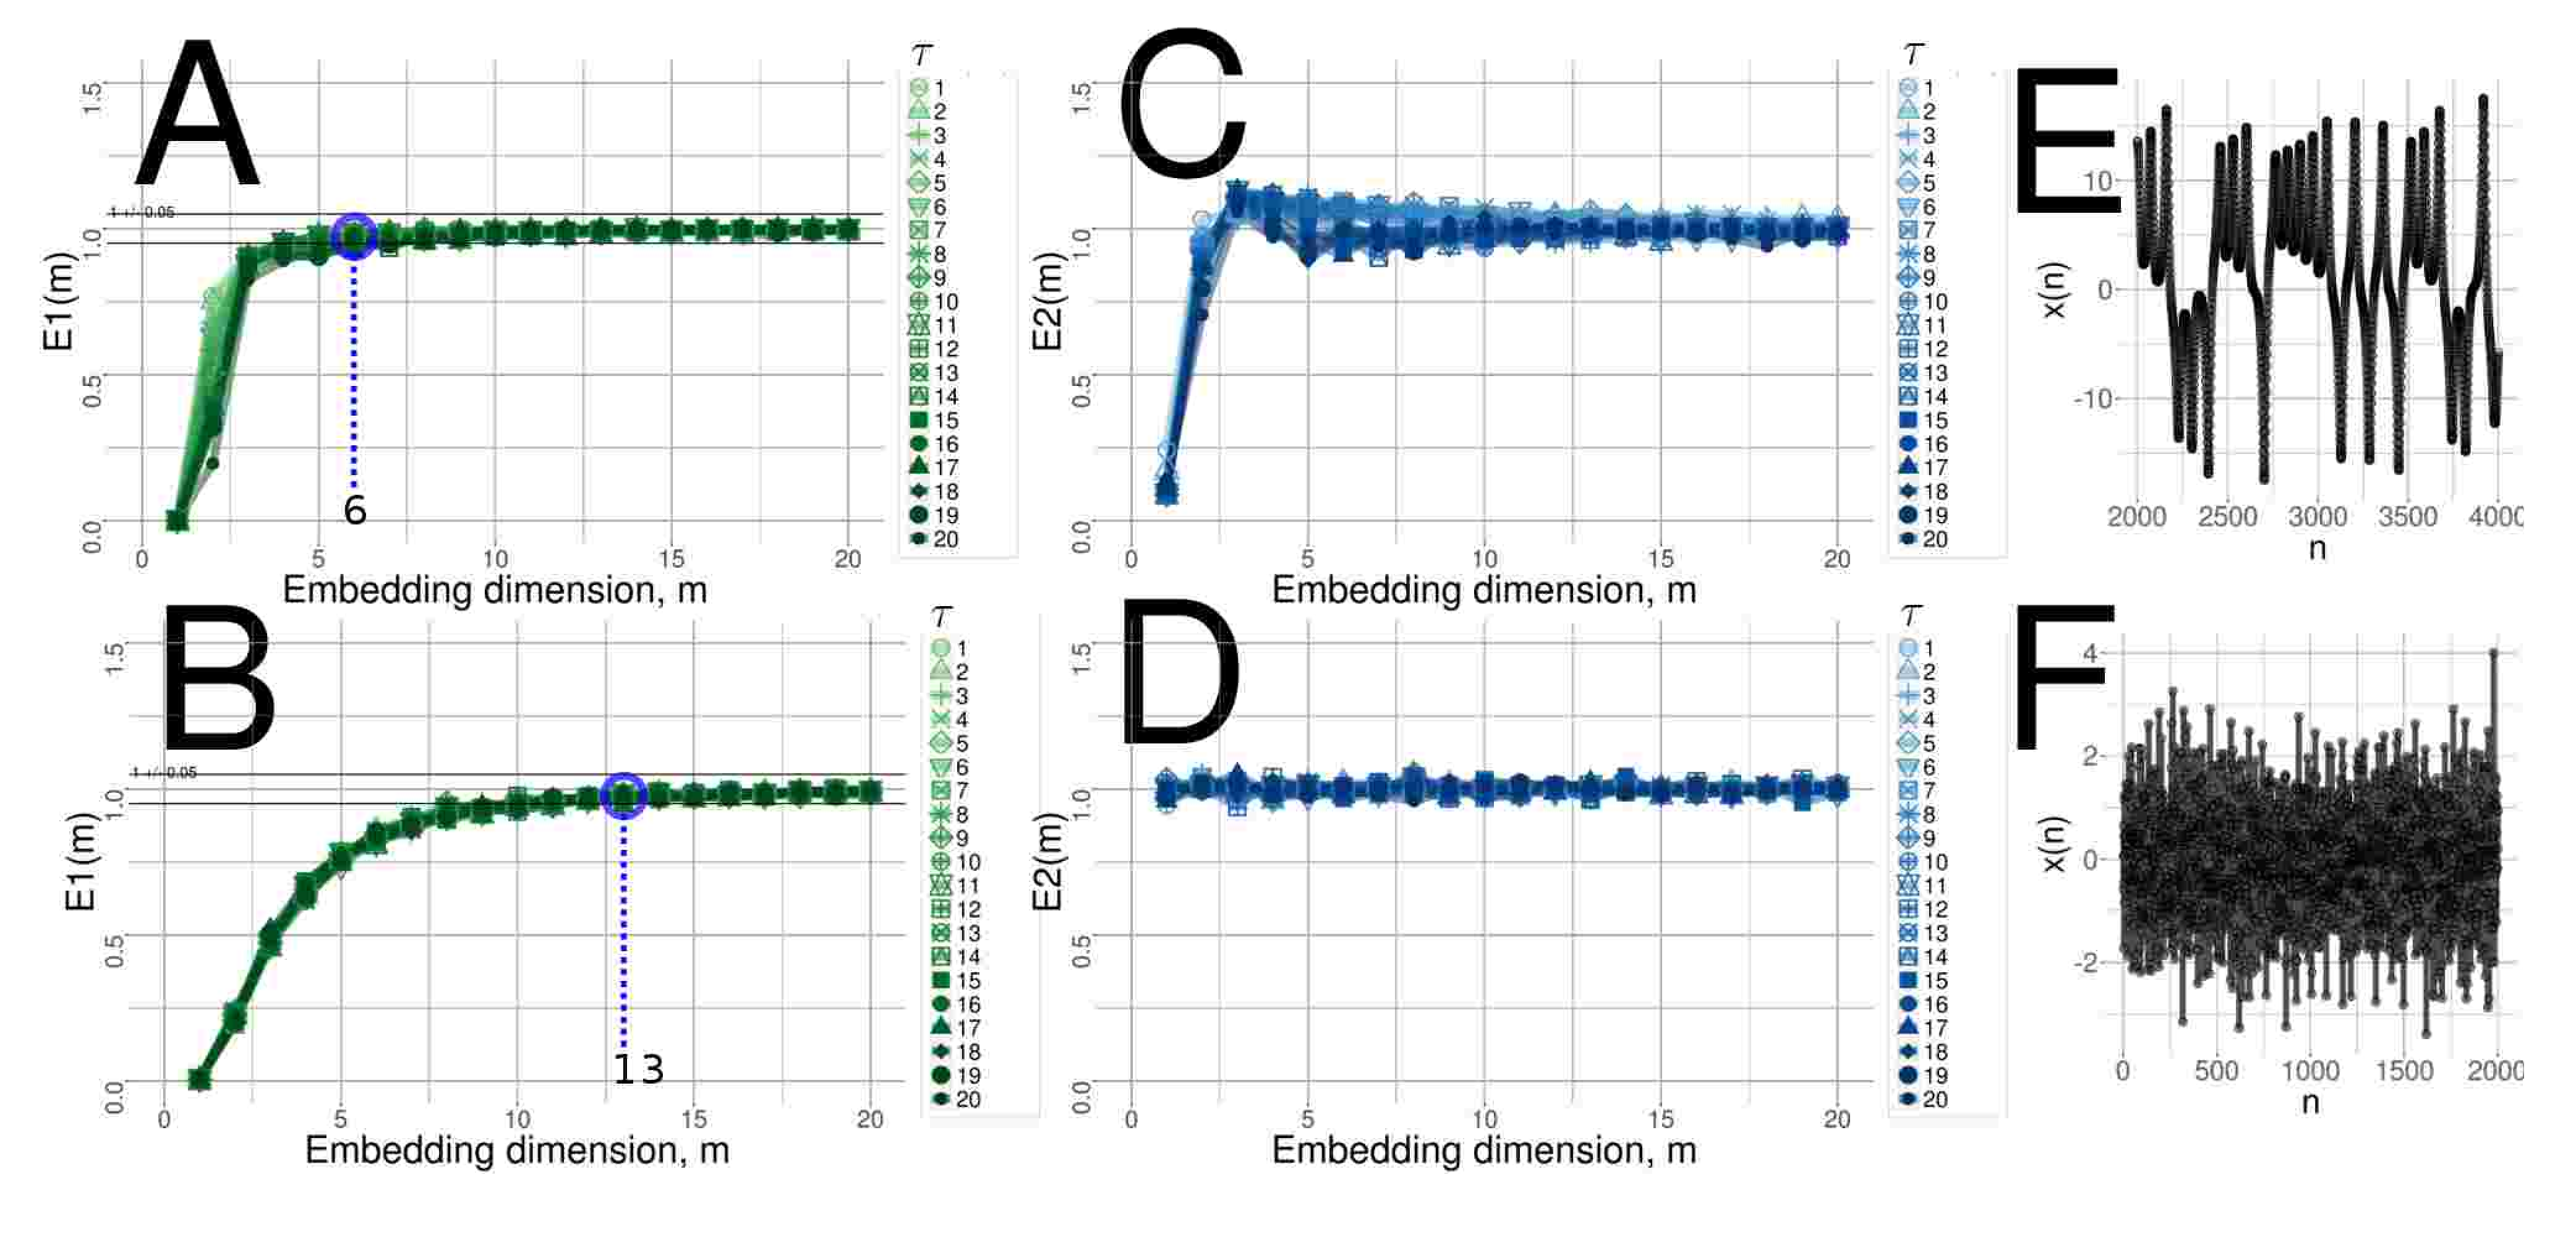
\includegraphics[width=1.0\textwidth]{figures/methods/cao/pdf/cao}
    \caption{
	{\bf Minimum dimension embedding values with Cao's method.} 
	(A, B) $E_1 (m)$ values and (C, D) $E_2(m)$ values 
	with variations of $\tau$ values from one to twenty
	for (E) chaotic and (F) random time series.
	Code and data to reproduce the figure is available from \cite{srep2019}.
        }
    \label{fig:e1e2}
\end{figure}
%%---------------------------------(FIGURE)-------------------------------------

It is important to note that for this work not only $E_1(m)$ and $E_2(m)$ are 
computed but also a variation of $\tau$ from 1 to 20 is presented. 
The purpose of such variation for $\tau$ is to show its independence with
regard to $E_1(m)$ and $E_2(m)$ values as $\tau$ is increasing 
(Fig~\ref{fig:e1e2}A,B,C, and D). 
However, one negative of the Cao's algorithm \cite{Cao1997} is the definition of 
a new threshold where $m$ values appear to be constant in $E_1 (m)$.
In the case of the given examples and reported results, we defined such 
threshold as 0.05. Further investigation is required for the selection of the 
threshold in the $E_1(m)$, as the selection of the threshold in this work is 
base on no particular method but visual inspection.

%%%%%%%%%%%%%%%%%%%%%%%%%%%%%%%%%%%%%%%%%%%%%%%%%%%%%%%%%%%%%%%%%%%%%%%%%%%%%%%%
%*******************************************************************************
\subsubsection*{Average Mutual Information}
When selecting the delay dimension parameter, $\tau$, one can consider the 
following two cases:
(i) when $\tau$ is too small, the elements of time-delay embedding will be along
the bisectrix of the phase space and the reconstruction is generally not 
satisfactory, 
(ii) on the contraty, when $\tau$ is too large the elements of the uniform 
time-delay embedding will become spread and uncorrelated which makes 
recovering the underlying attractor more difficult if not 
impossible \cite{casdagli1991, emrani2014a, garcia2005e71}.
With regard to the algorithms to compute $\tau$, 
Emrani et al. \cite{emrani2014a}, for instance, used the autocorrelation 
function in which the first zero crossing is considered as the minimum delay 
embedding parameter. However, the autocorrelation function is a linear 
statistic over which the Average Mutual Information (AMI) algorithm is 
preferred because the AMI takes into account the nonlinear dynamical 
correlations \cite{afraser1986,krakovska2015}. With this in mind, the AMI 
algorithm is described below to estimate the minimum delay embedding 
parameter, \texorpdfstring{$\tau_0$}{T}.

To compute the AMI, an histogram of $x(n)$ using $n$ bins is calculated
and then a probability distribution of data is computed \cite{kantz2003}.
AMI is therefore denoted by $I(\tau)$ which is the average mutual 
information between the original time series, $x(n)$, and the delayed 
time series, $x(n-\tau)$, delayed by $\tau$ \cite{kabiraj2012}. 
AMI is defined by
%%********************************[EQUATION]************************************
\begin{equation}\label{eq:ami}
I(\tau) = \sum_{i,j}^N p_{ij} log_2 \frac{ p_{ij} }{ p_i p_j }.
\end{equation}
%%********************************[EQUATION]************************************
Probabilities are defined as follows:
$p_i$ is the probability that $x(n)$ has a value inside the $i$-th bin of 
the histogram, $p_j$ is the probability that $x(n+\tau)$ has a value inside 
the $j$-th bin of the histogram and $p_{ij}(\tau)$ the probability 
that $x(n)$ is in bin $i$ and $x(n+\tau)$ is in bin $j$. The AMI is measured 
in bits (base 2, also called shannons) \cite{kantz2003, nonlinearTseries2016}.
For small $\tau$, AMI will be large and it will then decrease more or 
less rapidly. As $\tau$ increase and goes to a large limit, 
$x(n)$ and $x(n+\tau)$ have nothing to do with each other and $p_(ij)$ is 
factorised as $p_ip_j$ for which AMI is close to zero. Then, in order 
to obtain $\tau_0$, "it has to be found the first minimum of $I(\tau)$ 
where $x(n+\tau)$ adds maximal information to the knowledge from $x(n)$, or,
where the redundancy is the least" \cite{kantz2003}.

For example, we compute the AMI for two time series:
A) the $x$ solution of the Lorenz system, and
B) a noise time series using a normal distribution with mean zero and 
standard deviation equal to one. From Fig~\ref{fig:amis}, it can then be 
concluded that the amount of knowledge for any noise time series is zero 
for which the first minimum embedding parameter is $\tau_0=1$. 
On the contrary, the first minimum of the AMI for the chaotic time series 
is $\tau_0=17$ which is the value that maximize the independence 
between $x(n)$ and $x(n+\tau)$ in the reconstructed state space 
\cite{bradley2015}.
%%---------------------------------(FIGURE)-------------------------------------
\begin{figure}[ht]
\centering
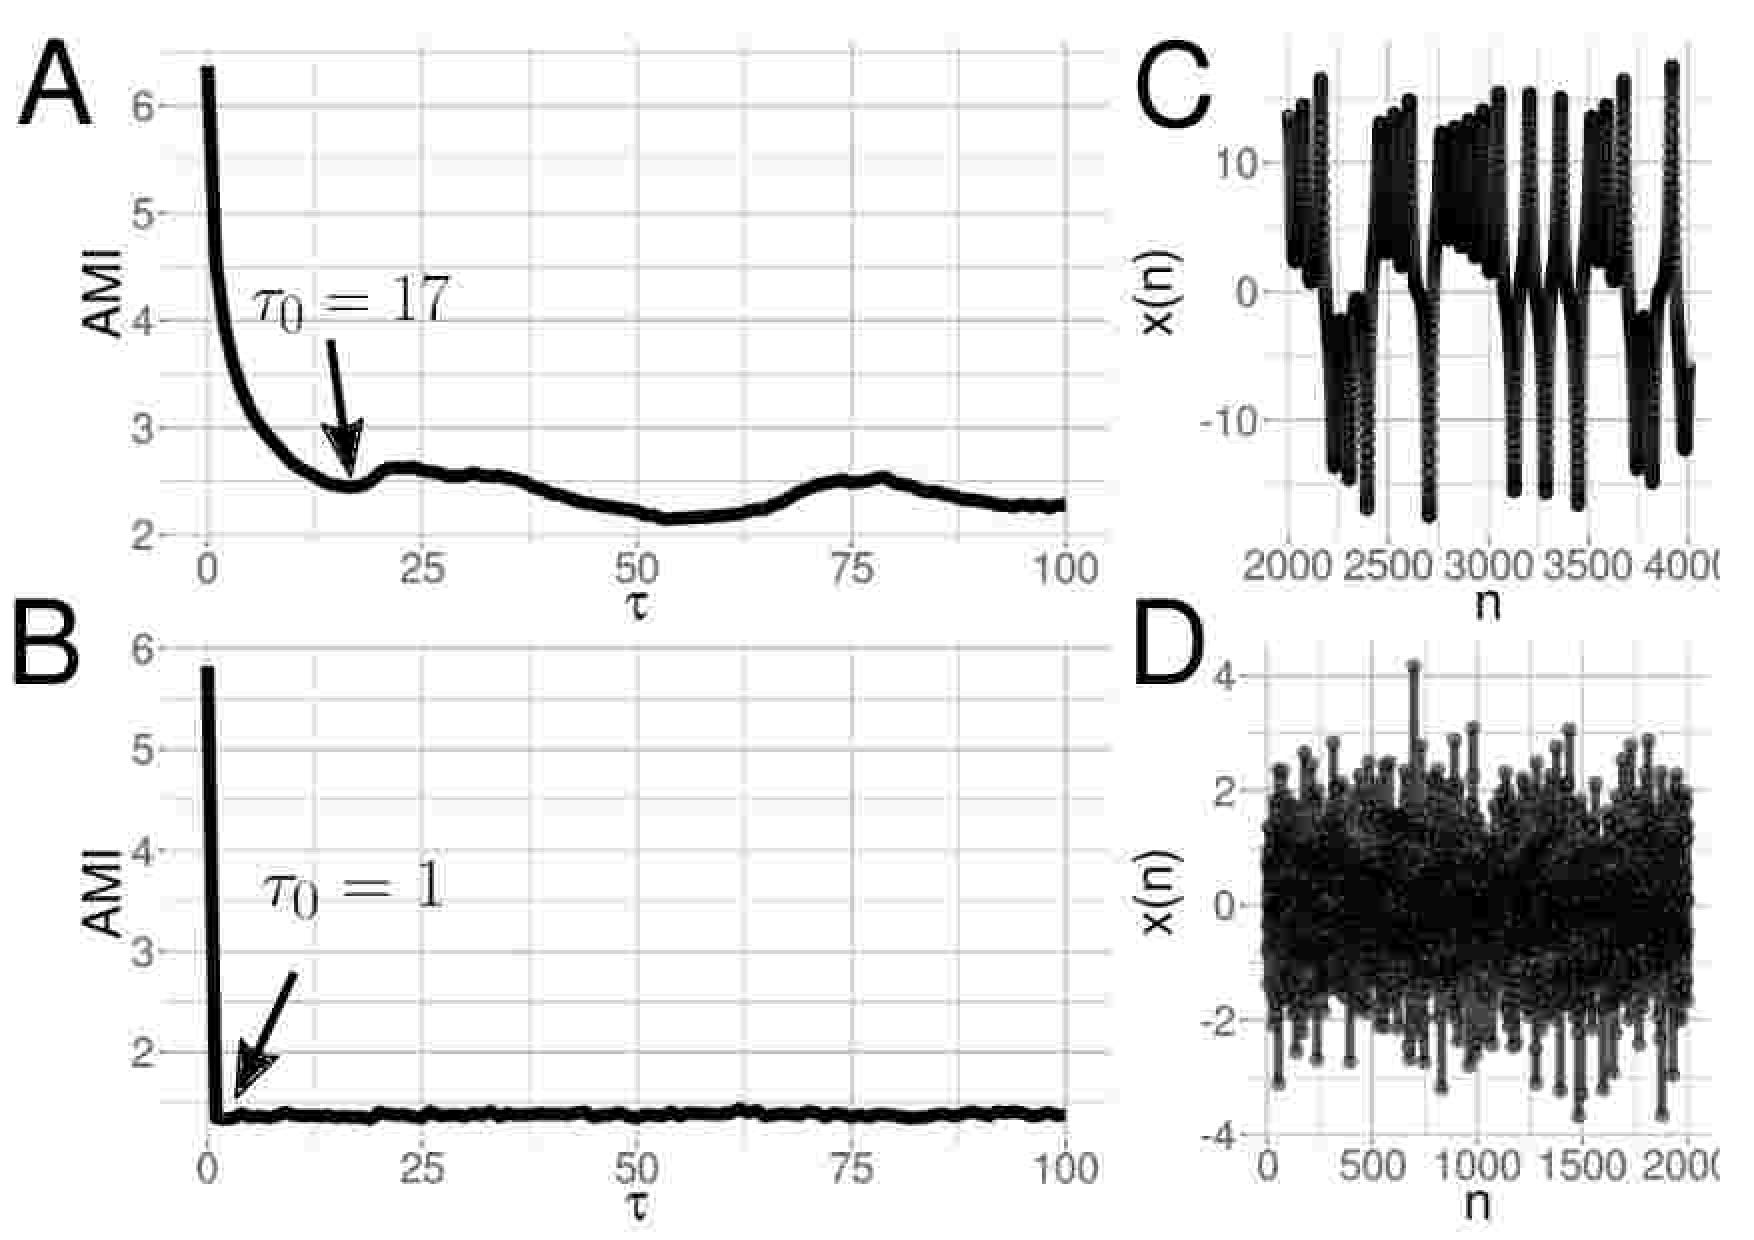
\includegraphics[width=1.0\textwidth]{figures/methods/ami/pdf/ami}
    \caption{
	{\bf Minimum delay embedding values with AMI's method.} 
    	(A, B) AMI values where its first minimum value in the curve
	is the minimum time delay embedding ($\tau_0$), 
	for (C) a chaotic and (D) noise time series.
	Code and data to reproduce the figure is available from \cite{srep2019}.
        }
    \label{fig:amis}
\end{figure}
%%---------------------------------(FIGURE)-------------------------------------
Similarly as Cao's algorithm negatives, AMI's algorithm is not an
exception for negatives, which are worthwhile to mention for further 
investigations.
For instance, (i) is not clear why the choose of the first minimum of the AMI 
is the minimum delay embedding parameter \cite{kantz2003} and 
(ii) the probability distribution of the AMI function is computed
with the use of histograms which depends on a heuristic choice of number of bins
for which AMI depends on partitioning \cite{garcia2005e71}.






%*******************************************************************************
\section*{Recurrence Quantification}\label{sec:recurrence-quantification}
\subsection*{Recurrence Plots}
Originally, Henri Poincar\'e in 1890 introduced the concept of recurrences 
in conservative systems, however such discovery was not put into practice 
until the development of faster computers \cite{marwan2007},
for which Eckmann et al. \cite{eckmann1987} in 1987 introduced a method
where recurrences in the dynamics of a system can be visualised using 
Recurrence Plots. The intention of Eckmann et al. \cite{eckmann1987} was to 
propose a tool, called Recurrence Plot (RP), that provides insights into 
high-dimensional dynamical systems where trajectories are very difficult to 
visualise. Therefore, "RP helps us to investigate the 
$m-$dimensional phase space trajectories through a two-dimensional 
representation of its recurrences" \cite{marwan2015}.
Similarly, Marwan et al. \cite{marwan2015} pointed out that additionally 
to the methodologies of the state space reconstruction and other dynamic 
invariants such as Lyapunov exponent, Kolmogorov-Sinai entropy, 
the recurrences of the trajectories in the phase space can provide 
important clues to characterise natural process that present, for
instance, periodicities (as Milankovitch cycles) or irregular cycles 
(as El Ni\~no Southern Oscillation). 
Such recurrences can not only be presented visually using Recurrence Plots (RP) 
but also be quantified with Recurrence Quantification metrics, which leads 
to applications of these in various areas such as economy, physiology, 
neuroscience, earth science, astrophysics and engineering \cite{marwan2007}.

For the creation of a recurrence plot based on time series 
$\{ \boldsymbol{x}_n \}$, it is first computed the state space 
reconstruction with uniform time-delay embedding 
$X(i)=\{ \boldsymbol{ \tilde{x} }_n, \dots,  
\boldsymbol{ \tilde{x} }_{n -(m-1)\tau} \}$
where $i=1,\dots,N$, $N$ is the number of considered states of $X(i)$ 
and $X(i) \in \mathbb{R}^m$ \cite{eckmann1987}.
The recurrence plot is therefore a two-dimensional $N \times N$ square 
matrix, $\mathbf{R}$, where a black dot is placed at $(i,j)$ 
whenever $X(i)$ is sufficiently close to $X(j)$: 
%%********************************[EQUATION]************************************
\begin{equation}
\mathbf{R}^{m}_{i,j} (\epsilon) = \Theta ( \epsilon_i - || X(i) - X(j) ||
\end{equation}
%%********************************[EQUATION]************************************
where $\quad i,j=1,\dots,N$, $\epsilon$ is a threshold distance, 
$|| \cdotp ||$ a norm, and $\Theta(\cdotp)$ is the Heaviside 
function (i.e. $\Theta(x)=0$, if $x<0$, and $\Theta(x)=1$ otherwise) 
(Fig~\ref{fig:mrp}) \cite{eckmann1987, marwan2007,marwan2015}.
RP is also characterised with a line of identity (LOI) which is a  
diagonal line due to $ R_{i,j}=1 (i,j=1,\dots,N)$. 
%---------------------------------(FIGURE)-------------------------------------
\begin{figure}[ht]
\centering
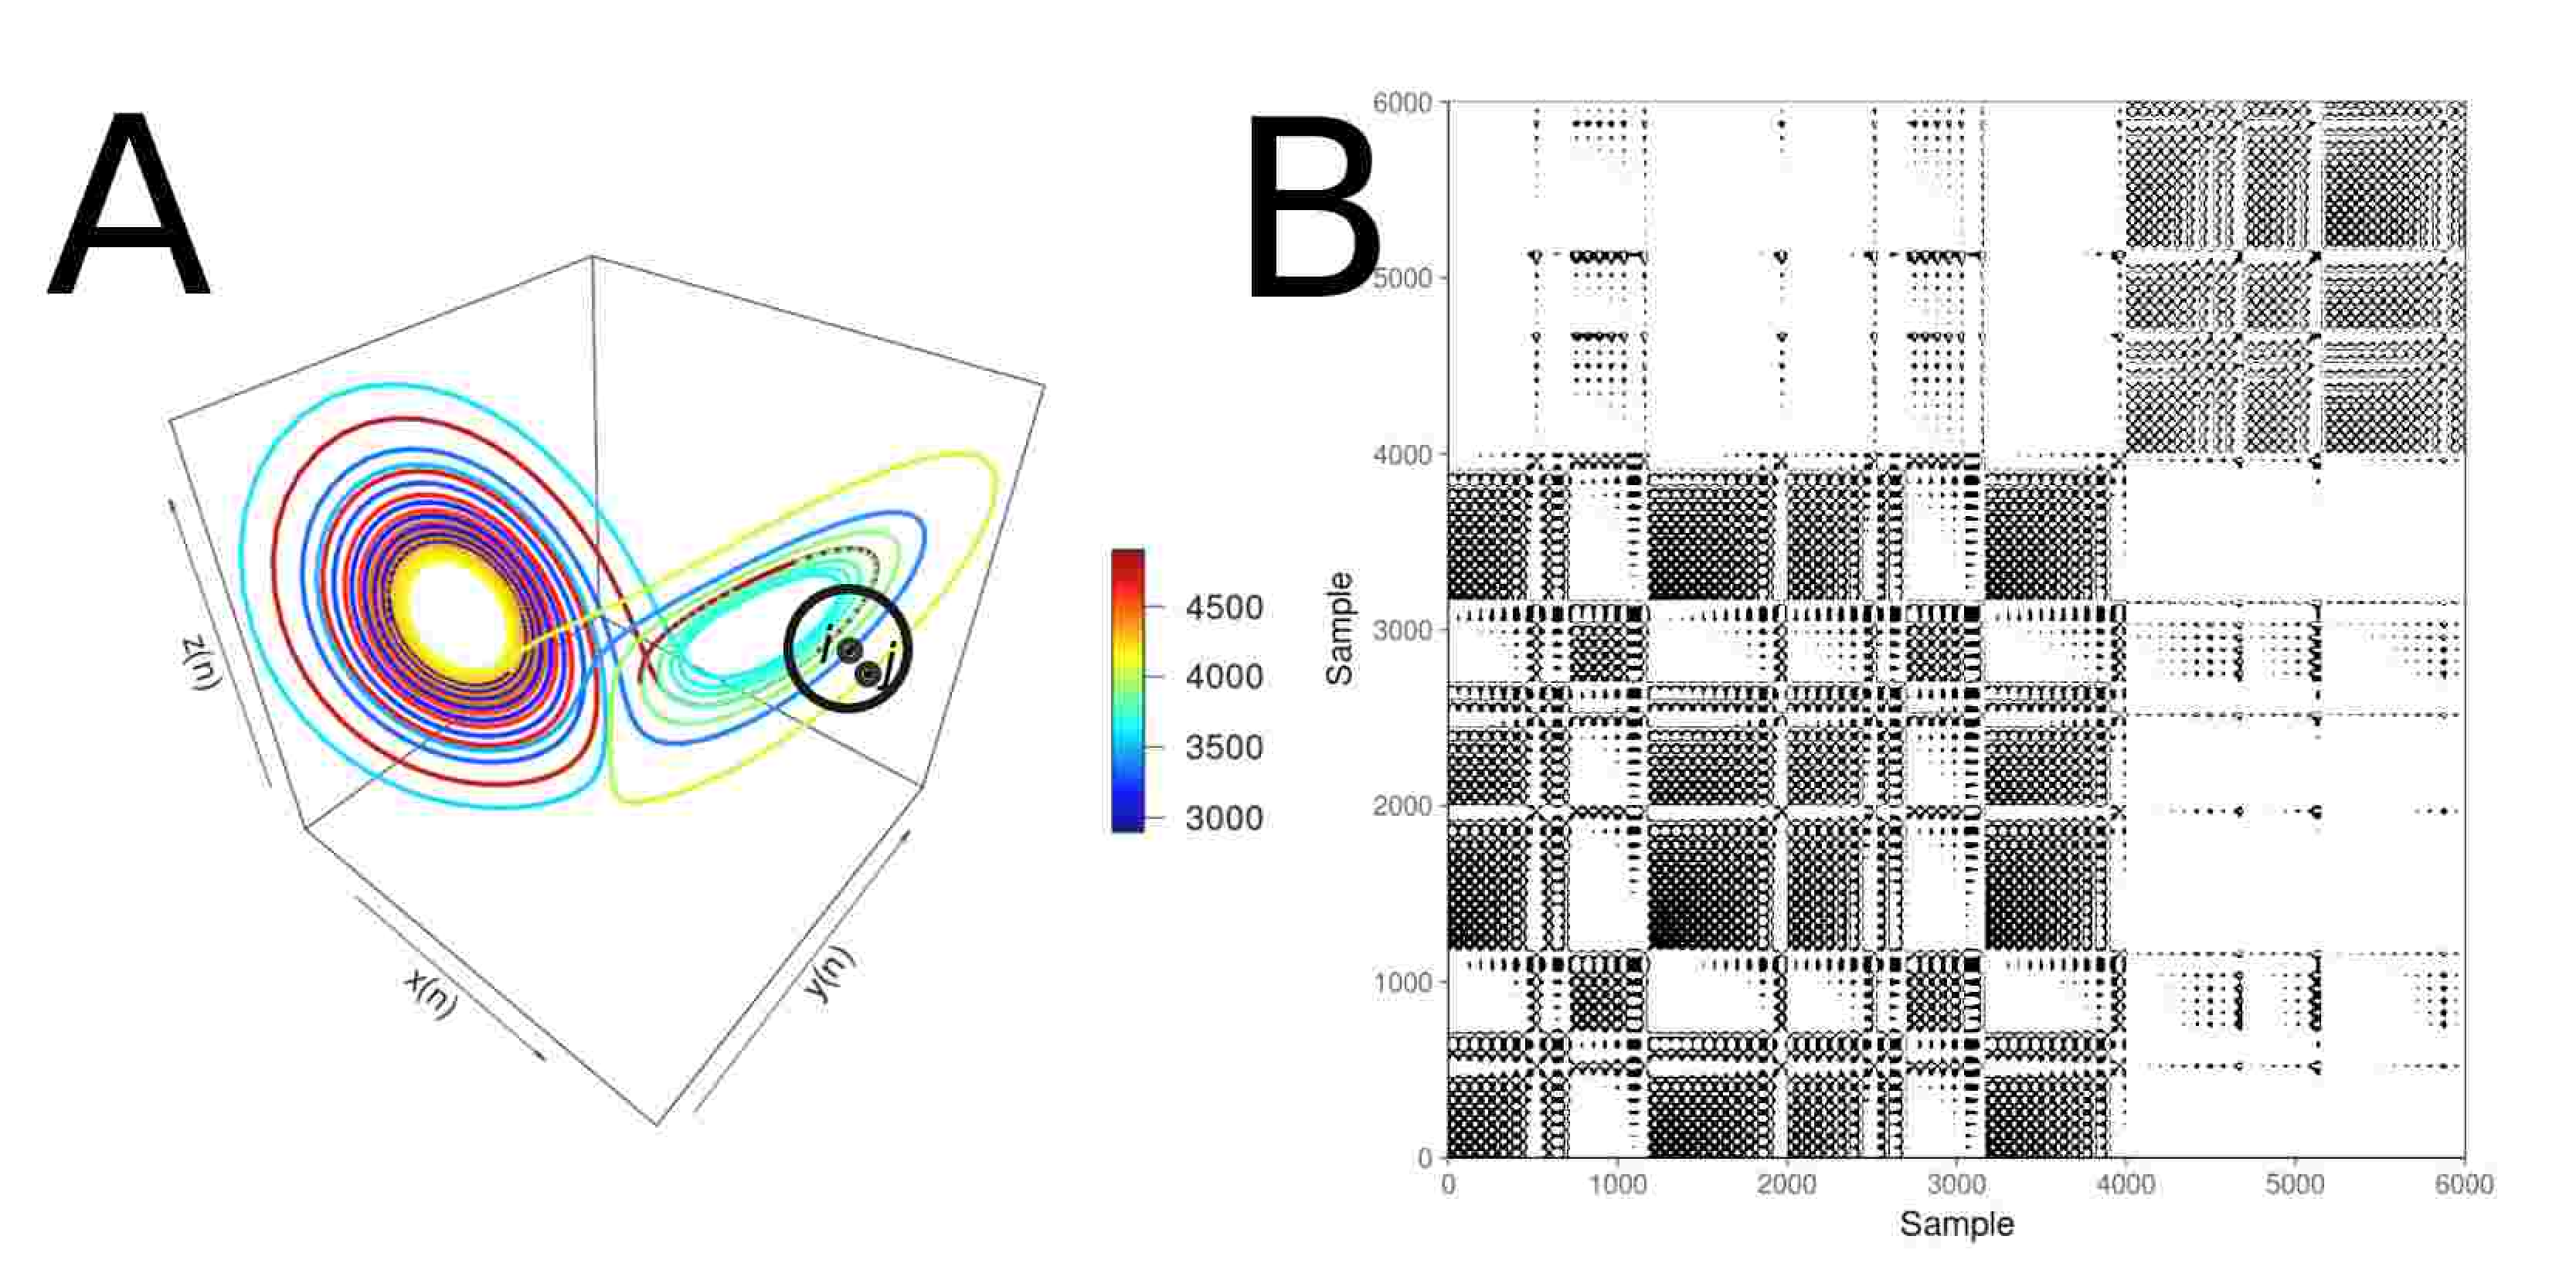
\includegraphics[width=1.0\textwidth]{figures/methods/rp/pdf/rp}
    \caption{
	{\bf Recurrence Plots.} 
	(A) State space of the Lorenz system with controlling parameters 
	($\rho=28, \sigma=10, \beta=8/3$). 
	A point, $j$, in trajectory $X()$ which falls into the neighborhood 
	(black circle) of a given point at $i$ is a recurrent point and is 
	represented as a black dot in the recurrence plot at location 
	$(i, j)$ or white otherwise.
	(B) Recurrence plot using the 
	three components of the Lorenz system and the RP with no embeddings 
	and threshold $\epsilon=5$.
	This figure is adapted from \cite{marwan2015}.
	Code and data to reproduce the figure is available from \cite{srep2019}.
	}
    \label{fig:mrp}
\end{figure}
%%---------------------------------(FIGURE)-------------------------------------





%*******************************************************************************
%*******************************************************************************
%*******************************************************************************
\subsection*{Structures of Recurrence Plots}
Pattern formations in the RPs can be designated either 
as topology for large-scale patterns or texture for small-scale patterns.
In the case of topology, the following pattern formations are commonly presented:
(i) homogeneous where uniform recurrence points are spread in the RP e.g., 
uniformly distributed noise (Fig~\ref{fig:rp2}A), 
(ii) periodic and quasi-periodic systems where diagonal lines and 
checkerboard structures represent oscillating systems, e.g., sinusoidal 
signals (Fig~\ref{fig:rp2}B), 
(iii) drift where paling or darkening recurrence points away from 
the LOI is caused by drifting systems, 
e.g., logistic map (Fig~\ref{fig:rp2}C), and
(iv) disrupted where recurrence points are presented white areas or 
bands that indicate abrupt changes in the dynamics, e.g. Brownian motion 
(Fig~\ref{fig:rp2}D) \cite{eckmann1987, marwan2015}.
Texture patterns in RPs can be categorised as:
(i) single or isolated recurrence points that represent rare occurring states, 
and do not persist for any time or fluctuate heavily,
(ii) dots forming diagonal lines where the length of the small-scale parallel 
lines in the diagonal are related to the ratio of determinism or predictability 
in the dynamics of the system, and
(iii) dots forming vertical and horizontal lines where the length of the 
lines represent a time length where a state does not change or change very 
slowly and these patterns formation represent discontinuities in the signal, 
and (iv) dots clustering to inscribe rectangular regions which are related 
to laminar states or singularities \cite{marwan2015}.
%%---------------------------------(FIGURE)-------------------------------------
\begin{figure}[ht]
\centering
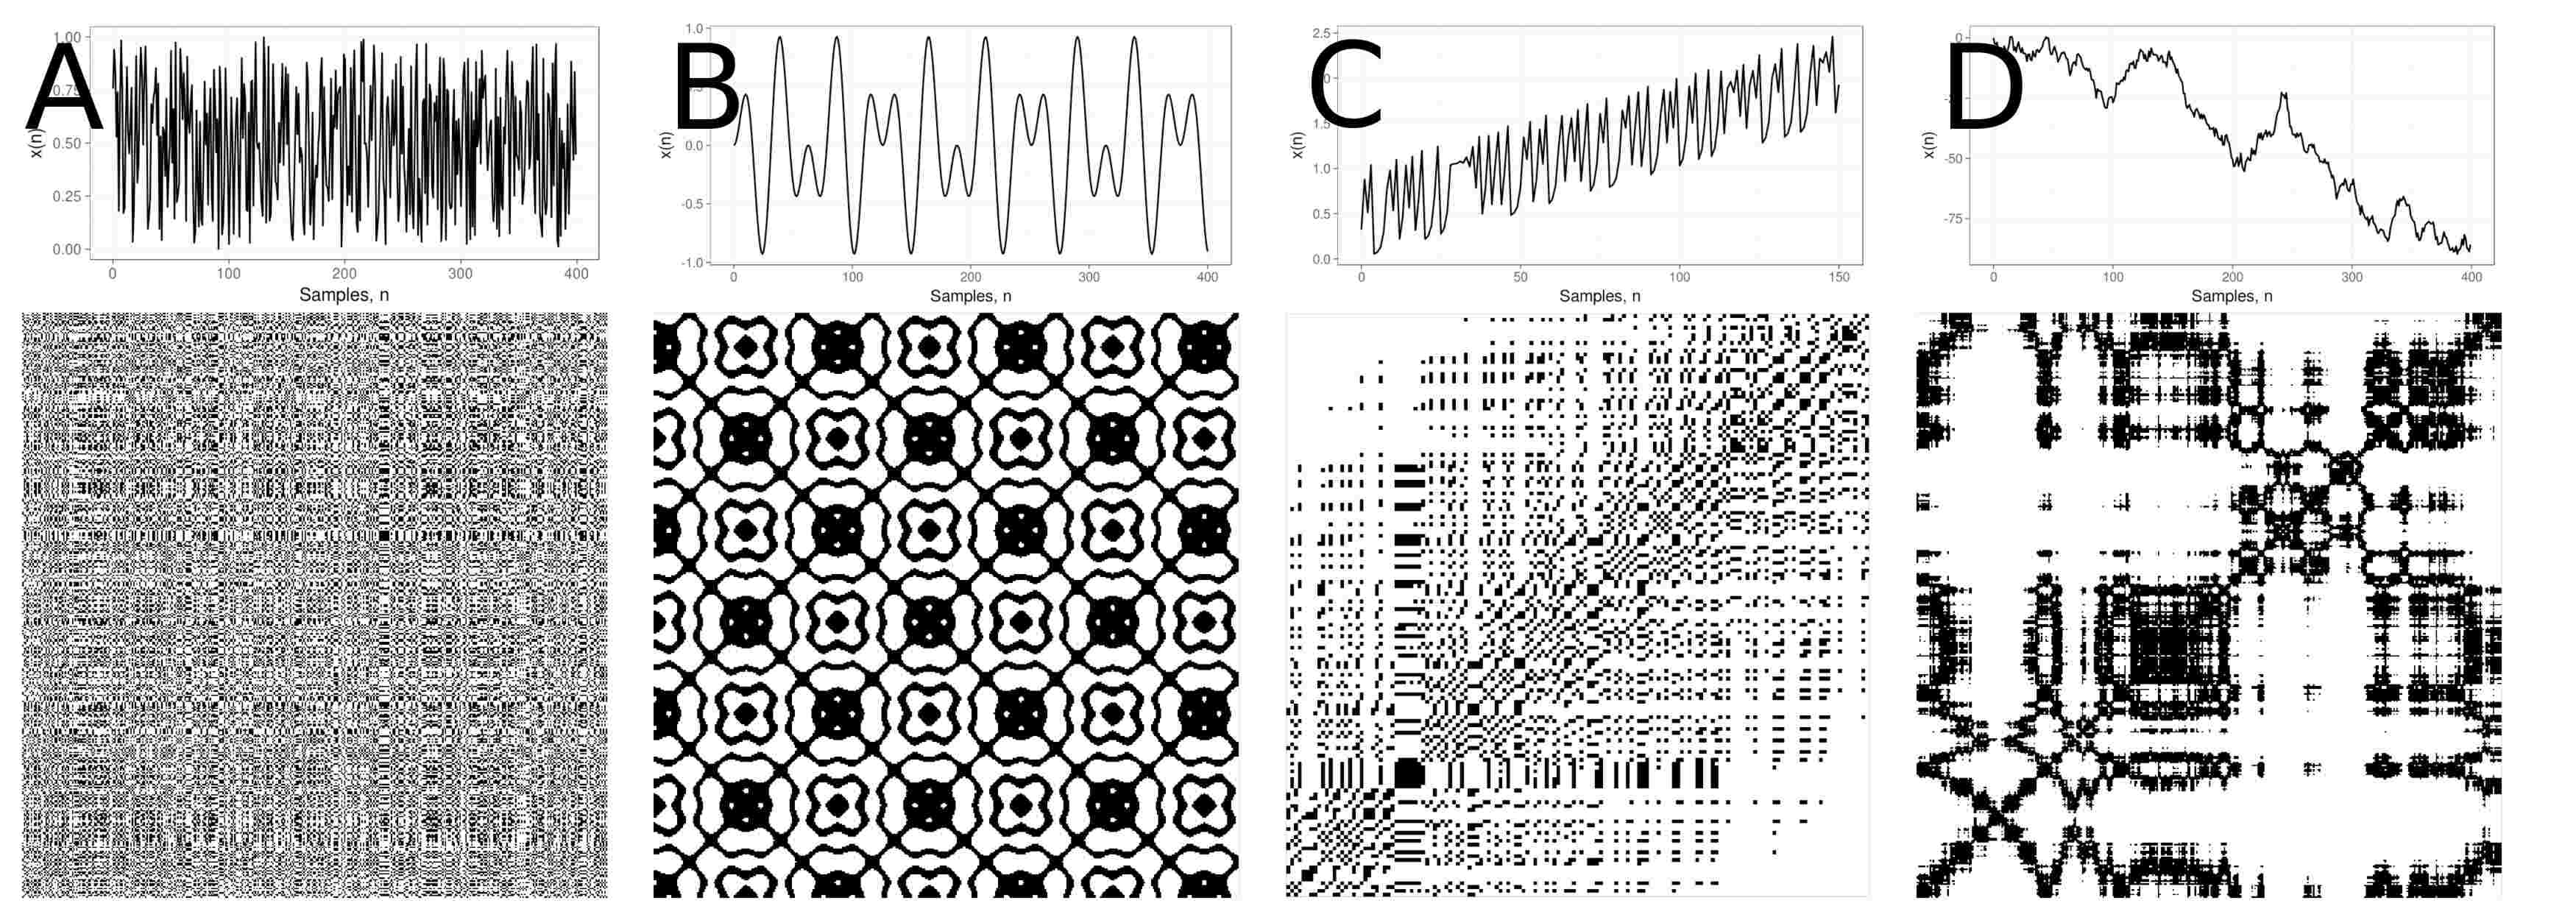
\includegraphics[width=1.0\textwidth]{figures/methods/rpsp/pdf/rpsp}
    \caption{
	{\bf Patterns in Recurrence Plots.} 
	Time-series with its respective recurrence plot for:
	(A) uniformly distributed noise,
	(B) super-positionet harmonic oscillation 
	($sin( \frac{1}{5}*t) * sin( \frac{5}{100}*t) $),
	(C) drift logistic map ($x_{i+1} = 4 x_i (1- x_i) $) corrupted 
	with a linearly increase term ($0.01*i$), and
	(D) disrupted brownian motion  ($x_{i+1} = x_i + 2*rnorm(1) $).
	This figure is adapted from \cite{marwan2015}.
	Code and data to reproduce the figure is available from \cite{srep2019}.
	}
    \label{fig:rp2}
\end{figure}
%%---------------------------------(FIGURE)-------------------------------------

Although, each of the previous pattern descriptions of the structures in the 
RP offer an idea of the characteristics of dynamical systems, 
these might be misinterpreted and conclusions might tend to be subjective 
as these require the interpretation of a particular researcher(s).
Because of that, recurrence quantification analyis (RQA) offer objective 
methodologies to quantify such visual characteristics of previous 
recurrent pattern structures in the RP \cite{zbilut1992}.

%*******************************************************************************
\subsection*{Recurrence Quantifications Analysis (RQA)}
Originally, Zbilut et al. \cite{zbilut1992} proposed metrics to investigate 
the density of recurrence points in RPs, then histograms of lengths for 
diagonal lines in RPs were studied by \cite{trulla1996} which were the 
introduction to the term recurrence quantification analysis (RQA) 
\cite{marwan2008}. RQA has been applied in many fields such as life science, 
engineering, physics, and others \cite{marwan2008}. Particularly in human 
movement to investigate noise and complexity of postural control 
\cite{rhea2011}, postural control \cite{apthorp2014} or interpersonal 
coordination \cite{duran2017}. The success of RQA is not only due to its 
simple algorithmic implementation but also to its capacity to detect tiny 
modulations in frequency or phase which are not detectable using standard 
methods e.g. spectral or wavelet analysis \cite{marwan2011}, and that 
RQA's metrics are quantitatively and qualitatively independe]nt of embedding 
dimension which is verified experimentally by \cite{iwanski1998}.
RQA metrics comprehend percentage of recurrence, percentage of determinism, 
ratio, Shannon entropy of the frequency distributions of the line lengths,
maximal line length and divergence, trend and laminariy 
\cite{marwan2007, marwan2015}. For this work, we considered only four 
RQA metrics, due to its consistency with our preliminary experiments, 
which are described below. Such metrics are computed the nonlinearTseries 
R package \cite{nonlinearTseries2016}.

\subsubsection*{REC values}
The percentage of recurrence (REC) is defined as
%%********************************[EQUATION]************************************
\begin{equation}
REC(\epsilon,N) = 
		\frac{1}{N^2 - N} \sum^{N}_{i \neq j = 1} 
		\mathbf{R}^{m}_{i,j}(\epsilon),
\end{equation}
%%********************************[EQUATION]************************************
which enumerates the black dots in the RP excluding the line of identity.
REC is a measure of the relative density of recurrence points in the sparse 
matrix \cite{marwan2015}.
%REC is computed as follow with the nonlinearTseries package 
% \cite{nonlinearTseries} 
%  hist = getHistograms(neighs, ntakens, lmin, vmin)
%  # calculate the number of recurrence points from the recurrence rate. The
%  # recurrence rate counts the number of points at every distance in a concrete
%  # side of the main diagonal.
%  # Thus, sum all points for all distances, multiply by 2 (count both sides) and
%  # add the maindiagonal
%  numberRecurrencePoints = sum(hist$recurrenceHist) + ntakens
%  # calculate the recurrence rate dividing the number of recurrent points at a
%  # given distance by all points that could be at that distance
%  recurrence_rate_vector = 
%  hist$recurrenceHist[1:(ntakens - 1)] / ((ntakens - 1):1)
%  # percentage of recurrent points
%  REC = (numberRecurrencePoints) / ntakens ^ 2

\subsubsection*{DET values} 
The percent determinism (DET) is defined as the fraction of recurrence points
that form diagonal lines and it is determined by
%%********************************[EQUATION]************************************
\begin{equation}
DET=
	\frac{\sum^{N}_{l=d_{min}} l H_D{l} }
	     {\sum^{N}_{i,j=1} \mathbf{R}_{i,j}(\epsilon) },
\end{equation}
%%********************************[EQUATION]************************************
where 
%%********************************[EQUATION]************************************
\begin{equation}
H_D(l) = 
	\sum^{N}_{i,j=1} 
	(1- \mathbf{R}_{i-1,j-1}(\epsilon) ) 
	(1- \mathbf{R}_{i+l,j+l}(\epsilon) ) 
	\prod^{l-1}_{k=0}  \mathbf{R}_{i+k,j+k}(\epsilon)
\end{equation}
%%********************************[EQUATION]************************************
is the histogram of the lengths of the diagonal structures in the RP.
DET can be interpreted as the predictability of the system for periodic signals 
which, in essence, have longer diagonal lines than the short diagonals lines
for chaotic signals or absent diagonal lines for stochastic signals 
\cite{marwan2007, marwan2015}. Similarly, DET is considered as a measurement for 
the organisation of points in RPs  \cite{iwanski1998}. 
%percent determinism (DET) is computed as follow with the nonlinearTseries 
%package \cite{nonlinearTseries}  
% calculateDiagonalParameters = function(ntakens, numberRecurrencePoints,
%                                       lmin = 2, lDiagonalHistogram,
%                                       recurrence_rate_vector, maxDistanceMD) {
%  #begin parameter computations
%  num = sum((lmin:ntakens) * lDiagonalHistogram[lmin:ntakens])
%  DET = num / numberRecurrencePoints


\subsubsection*{RATIO values}
RATIO is defined as the ratio between DET and REC and it is calculated from 
the frequency distributions of the lengths of the diagonal lines.
RATIO is useful to discover dynamic transitions \cite{marwan2015}.
%  diagP = calculateDiagonalParameters(
%    ntakens, numberRecurrencePoints, lmin, hist$diagonalHist,
%    recurrence_rate_vector, maxDistanceMD
%  )
% calculateDiagonalParameters = function(ntakens, numberRecurrencePoints,
%                                       lmin = 2, lDiagonalHistogram,
%                                       recurrence_rate_vector, maxDistanceMD) {
%  #begin parameter computations
%  num = sum((lmin:ntakens) * lDiagonalHistogram[lmin:ntakens])
%  DET = num / numberRecurrencePoints
% 
%
%    RATIO = diagP$DET / REC
%

\subsubsection*{ENT values}
ENT is the Shannon entropy of the frequency distribution of the diagonal 
line lengths and it is defined as
%%********************************[EQUATION]************************************
\begin{equation}
ENT= - \sum^{N}_{l=d_{min}} p(l) ln p(l) \quad with 
	\quad p(l)=\frac{ H_D(l) }{ \sum^{N}_{ l=d_{min} } H_D(l) }.
\end{equation}
%%********************************[EQUATION]************************************
ENT reflects the complexity of the deterministic structure in the system.
For instance, for uncorrelated noise or oscillations, 
the value of ENT is rather small and indicates low complexity of the system,
therefore "the higher the ENT is the more complex the dynamics are" 
\cite{marwan2007, marwan2015}.
%#'  \item \emph{ENTR}: Shannon entropy of the diagonal line lengths distribution
%
%calculateDiagonalParameters = function(ntakens, numberRecurrencePoints,
%                                       lmin = 2, lDiagonalHistogram,
%                                       recurrence_rate_vector, maxDistanceMD) {
%
%  pl = lDiagonalHistogram / sum(lDiagonalHistogram)
%  diff_0 = which(pl > 0)
%  ENTR = -sum(pl[diff_0] * log(pl[diff_0]))

 
\subsection*{Sensitivity and robustness of RPs and RQA.}
RP and RQA are a very young field in nonlinear dynamics and many questions 
are still open, for instance, different parameters for window length size 
of the time series, embedding parameters or recurrence threshold can 
generate different results in RQA's metrics \cite{marwan2011, eckmann1987}.

The selection of recurrence threshold, $\epsilon$, can depend on the system 
that is analysed. For instance, when studying dynamical invariants $\epsilon$ 
require to be very small, for trajectory reconstruction $\epsilon$ requires 
to have a large thresholds or when studying dynamical transition 
there is little importance about the selection of the threshold 
\cite{marwan2011}. Other criteria for the selection of $\epsilon$ is that 
the recurrence threshold  should be five times larger 
than the standard deviation of the observational noise
or the use of diagonal structures within the RP is suggested in order
to find the optimal recurrence threshold for (quasi-)periodic process 
\cite{marwan2011}.

Similarly, Iwanski et al. \cite{iwanski1998} highlighted the importance 
of choosing the right embedding parameters to perform RQA for which 
many experiments have to be performed using different parameters in order 
to have a better intuition of the nature of the time series and how 
this is represented by using RQA.

With that in mind, this work explores the sensitivity and robustness 
of the window size of time series, embedding parameters for RSS with UTDE 
and recurrence threshold for RP and RQA in order to gain a better insight 
into the underlying time series collected from inertial sensors in the 
context of human-humanoid imitation activities.







%*******************************************************************************
%*******************************************************************************
%*******************************************************************************
\section*{Experiment} \label{sec:experiment}
We conducted an experiment in the context of human-humanoid imitation (HHI) 
activities where participants were asked to imitate simple horizontal and 
vertical arm movements performed by NAO, a humanoid robot \cite{gouaillier2009}.
Such simple movements were repeated ten times for the participant 
who copied NAO's arm movements in a face-to-face imitation activity.
Also, wearable inertial measurement unit (IMU) sensors were attached 
to the right hand of the participant and to the left hand of the robot 
(Figure~\ref{fig:hri} A,C). Data were then collected with four NeMEMSi 
IMU sensors with sampling rate of 50Hz provinding tri-axial data of the 
accelerometer, gyroscope and magnetometer sensors and quaternions 
\cite{Comotti2014}. 
%A further description of the NeMEMSi IMU sensors 
%is given in \nameref{S1_AppendixB}.
%%---------------------------------(FIGURE)-------------------------------------
\begin{figure}[ht]
  \centering
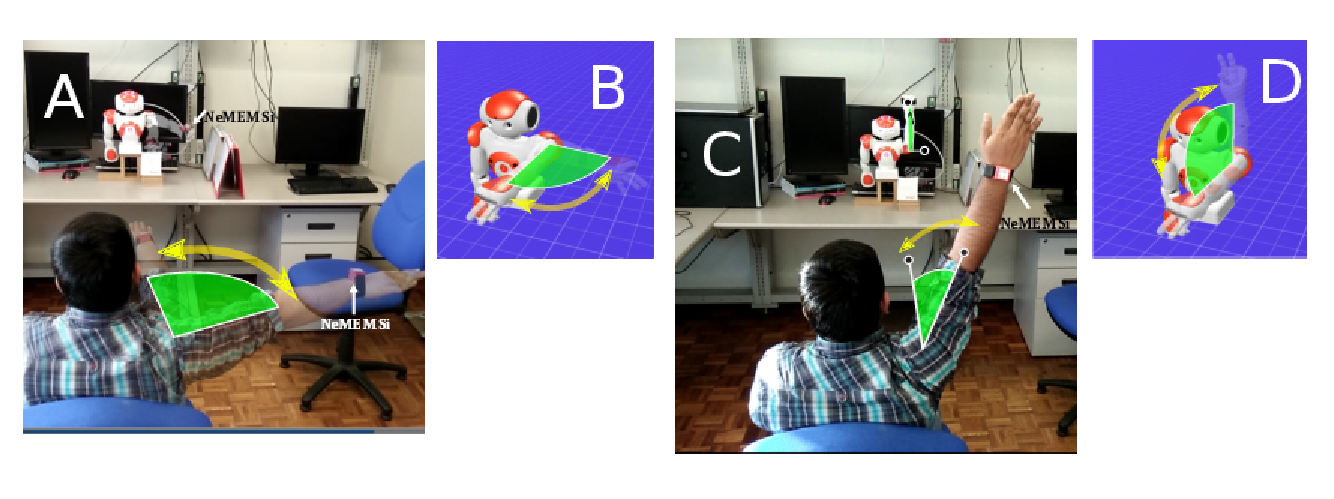
\includegraphics[width=1.0\textwidth]{figures/experiment/hri/pdf/hri}
    \caption{
	{\bf Human-humanoid imitation activities.} 
    		Face-to-face human-humanoid imitation (HHI) activities for 
		(A) HHI of horizontal arm movement, 
		(B) Humanoid horizontal arm movement,
		(C) HHI of vertical arm movement, and 
		(D) Humanoid vertical arm movement.
        }
    \label{fig:hri}
\end{figure}
%%---------------------------------(FIGURE)------------------------------------

\subsection*{Participants}
Twenty-three participants,
from now on defined as $pN$ where $N$ is the number of participant, were 
invited to do the experiment. However, data for three participants were 
not used because the instructions for $p01$, who was the only left-handed,
were mistakenly given in a way that movements were performed different
from what had been planned, and for participants $p13$ and $p16$ 
data were corrupted because bluetooth communications problems with the 
sensors. With that in mind, data for twenty participants were analysed in 
this work.

Of the twenty participants, all of them are right-handed healthy participants 
of whom four are females and sixteen are males with a mean and standard 
deviation (SD) age of mean=19.8 (SD=1.39). All participants provided 
informed consent forms prior to participation in the experiment.

\subsection*{Human-humanoid imitation activities}
For human-humanoid imitation (HHI) activities four neMEMSi sensors were used,
two of which were attached to the right hand of the participant and the 
other two to the left hand of the humanoid robot.
Then, each participant was asked to imitate repetitions of simple horizontal
and vertical arm movements performed by the humanoid robot in the following 
conditions:
(i) ten repetitions of horizontal arm movement at normal (HN) 
	and faster (HF) speed (Figure~\ref{fig:hri} A), and
(ii) ten repetitions of vertical arm movement at normal (VN) 
	and faster (VF) speed (Figure~\ref{fig:hri} C).
The normal and faster speed of arm movements is defined by the duration 
in number of samples of one repetition of NAO's arm movements. 
We select NAO's arm movements duration to distinguish between normal and 
faster arm movements as NAO's movements have less variation between 
repetition to repetition. The duration for one repetition of the horizontal 
arm movement at normal speed, HN, is about 5 seconds considering 
that each repetition last around 250 samples.
For horizontal arm movement at faster speed, HF, each repetition were performed 
in around 2 seconds which correspond to 90 samples of data.
The vertical arm movement at normal speed, VN, were performed  in 6 seconds 
which is around 300 samples of data. For vertical arm movement at 
faster speed, VF, each repetition lasts about 2.4 seconds which correspond 
to 120 samples of data.
To visualise the distinction between normal and faster speed for horizontal 
and vertical arm movements, Fig~\ref{fig:sts} shows smoothed time series 
for axes Z and Y of the gyroscope sensors with four window lengths: 
2-sec (100-samples), 5-sec (250-samples), 10-sec (500-samples) 
and 15-sec (750-samples).
%%---------------------------------(FIGURE)-------------------------------------
\begin{figure}[ht] 
\centering
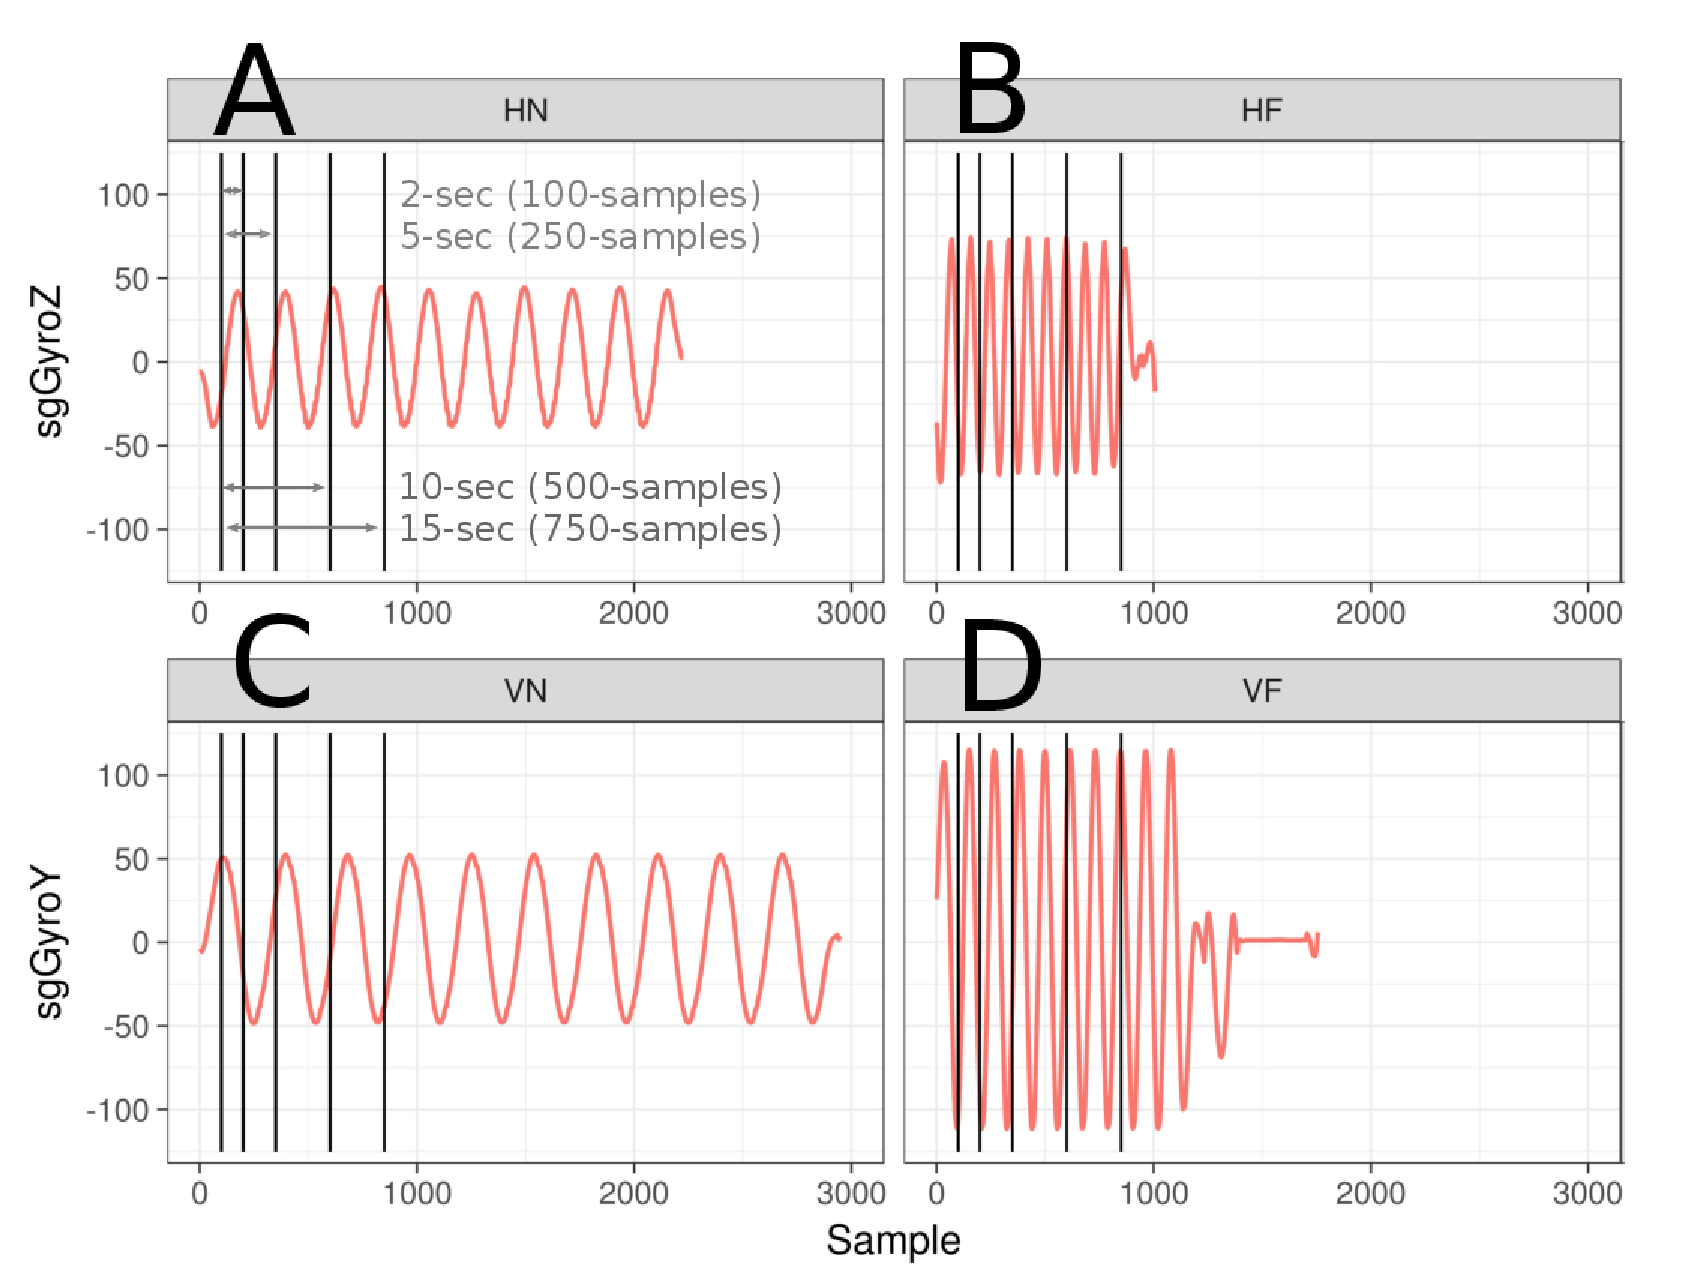
\includegraphics[width=1.0\textwidth]{figures/experiment/sts/pdf/sts}
    \caption{
	{\bf Time series duration of horizontal and vertical arm movements.} 
    		Time series of smoothed data from gyroscope sensor 
		for different speed arm movements performed by NAO: 
		(A) Horizontal Normal arm movement (HN), 
		(B) Horizontal Faster arm movement (HF),
		(C) Vertical Normal arm movement (VN) and 
		(D) Vertical Faster arm movement (VF).
		Additionally, 
		(A) shows window sizes for 2-seconds (100 samples), 
		5-seconds (250 samples), 10-seconds (500 samples) 
		and 15-seconds (750 samples)
		which are also presented in (B), (C) and (D).
		Code and data to reproduce the figure is available from \cite{srep2019}.
        }
	\label{fig:sts}
\end{figure}
%%---------------------------------(FIGURE)------------------------------------




\subsection*{Data from Inertial Measurement Units} 
	\label{sec:experiment:subsec:imu}


To give insight to the research questions, 
we considered various conditions of time series collected for this work 
(see Experiment section for more details) which are described as follows
\begin{itemize}
\item Three levels of smoothness for the normalised data 
	(sg0zmuv, sg1zmuv and sg2zmuv), computed from two different filter 
	lengths (29 and 159) with the same polynomial degree 
	of 5 using the function \texttt{sgolay(p,n,m)} \cite{Rsignal},
\item four velocities arm movement activities: 
	horizontal normal (HN), horizontal faster (HF), 
	vertical normal (VN), and vertical faster (VF), and
\item four window lengths: 2-sec (100 samples), 5-sec (250 samples), 
	10-sec (500 samples) and 15-sec (750 samples).
\end{itemize}
%\subsection*{Time series}
After the data collection, raw time series were windowed, normalised and 
smoothed. Then, due to space limitations and to have simple visualisation, 
we only present 10-sec (500 samples) window length time series for 
three participants (p01, p01 and p03) performing horizontal 
arm movements (axis GyroZ) and vertical arm movements (axis GyroY) (Figs \ref{fig:ts}). 
%%---------------------------------(FIGURE)-------------------------------------
\begin{figure}[ht]
\centering
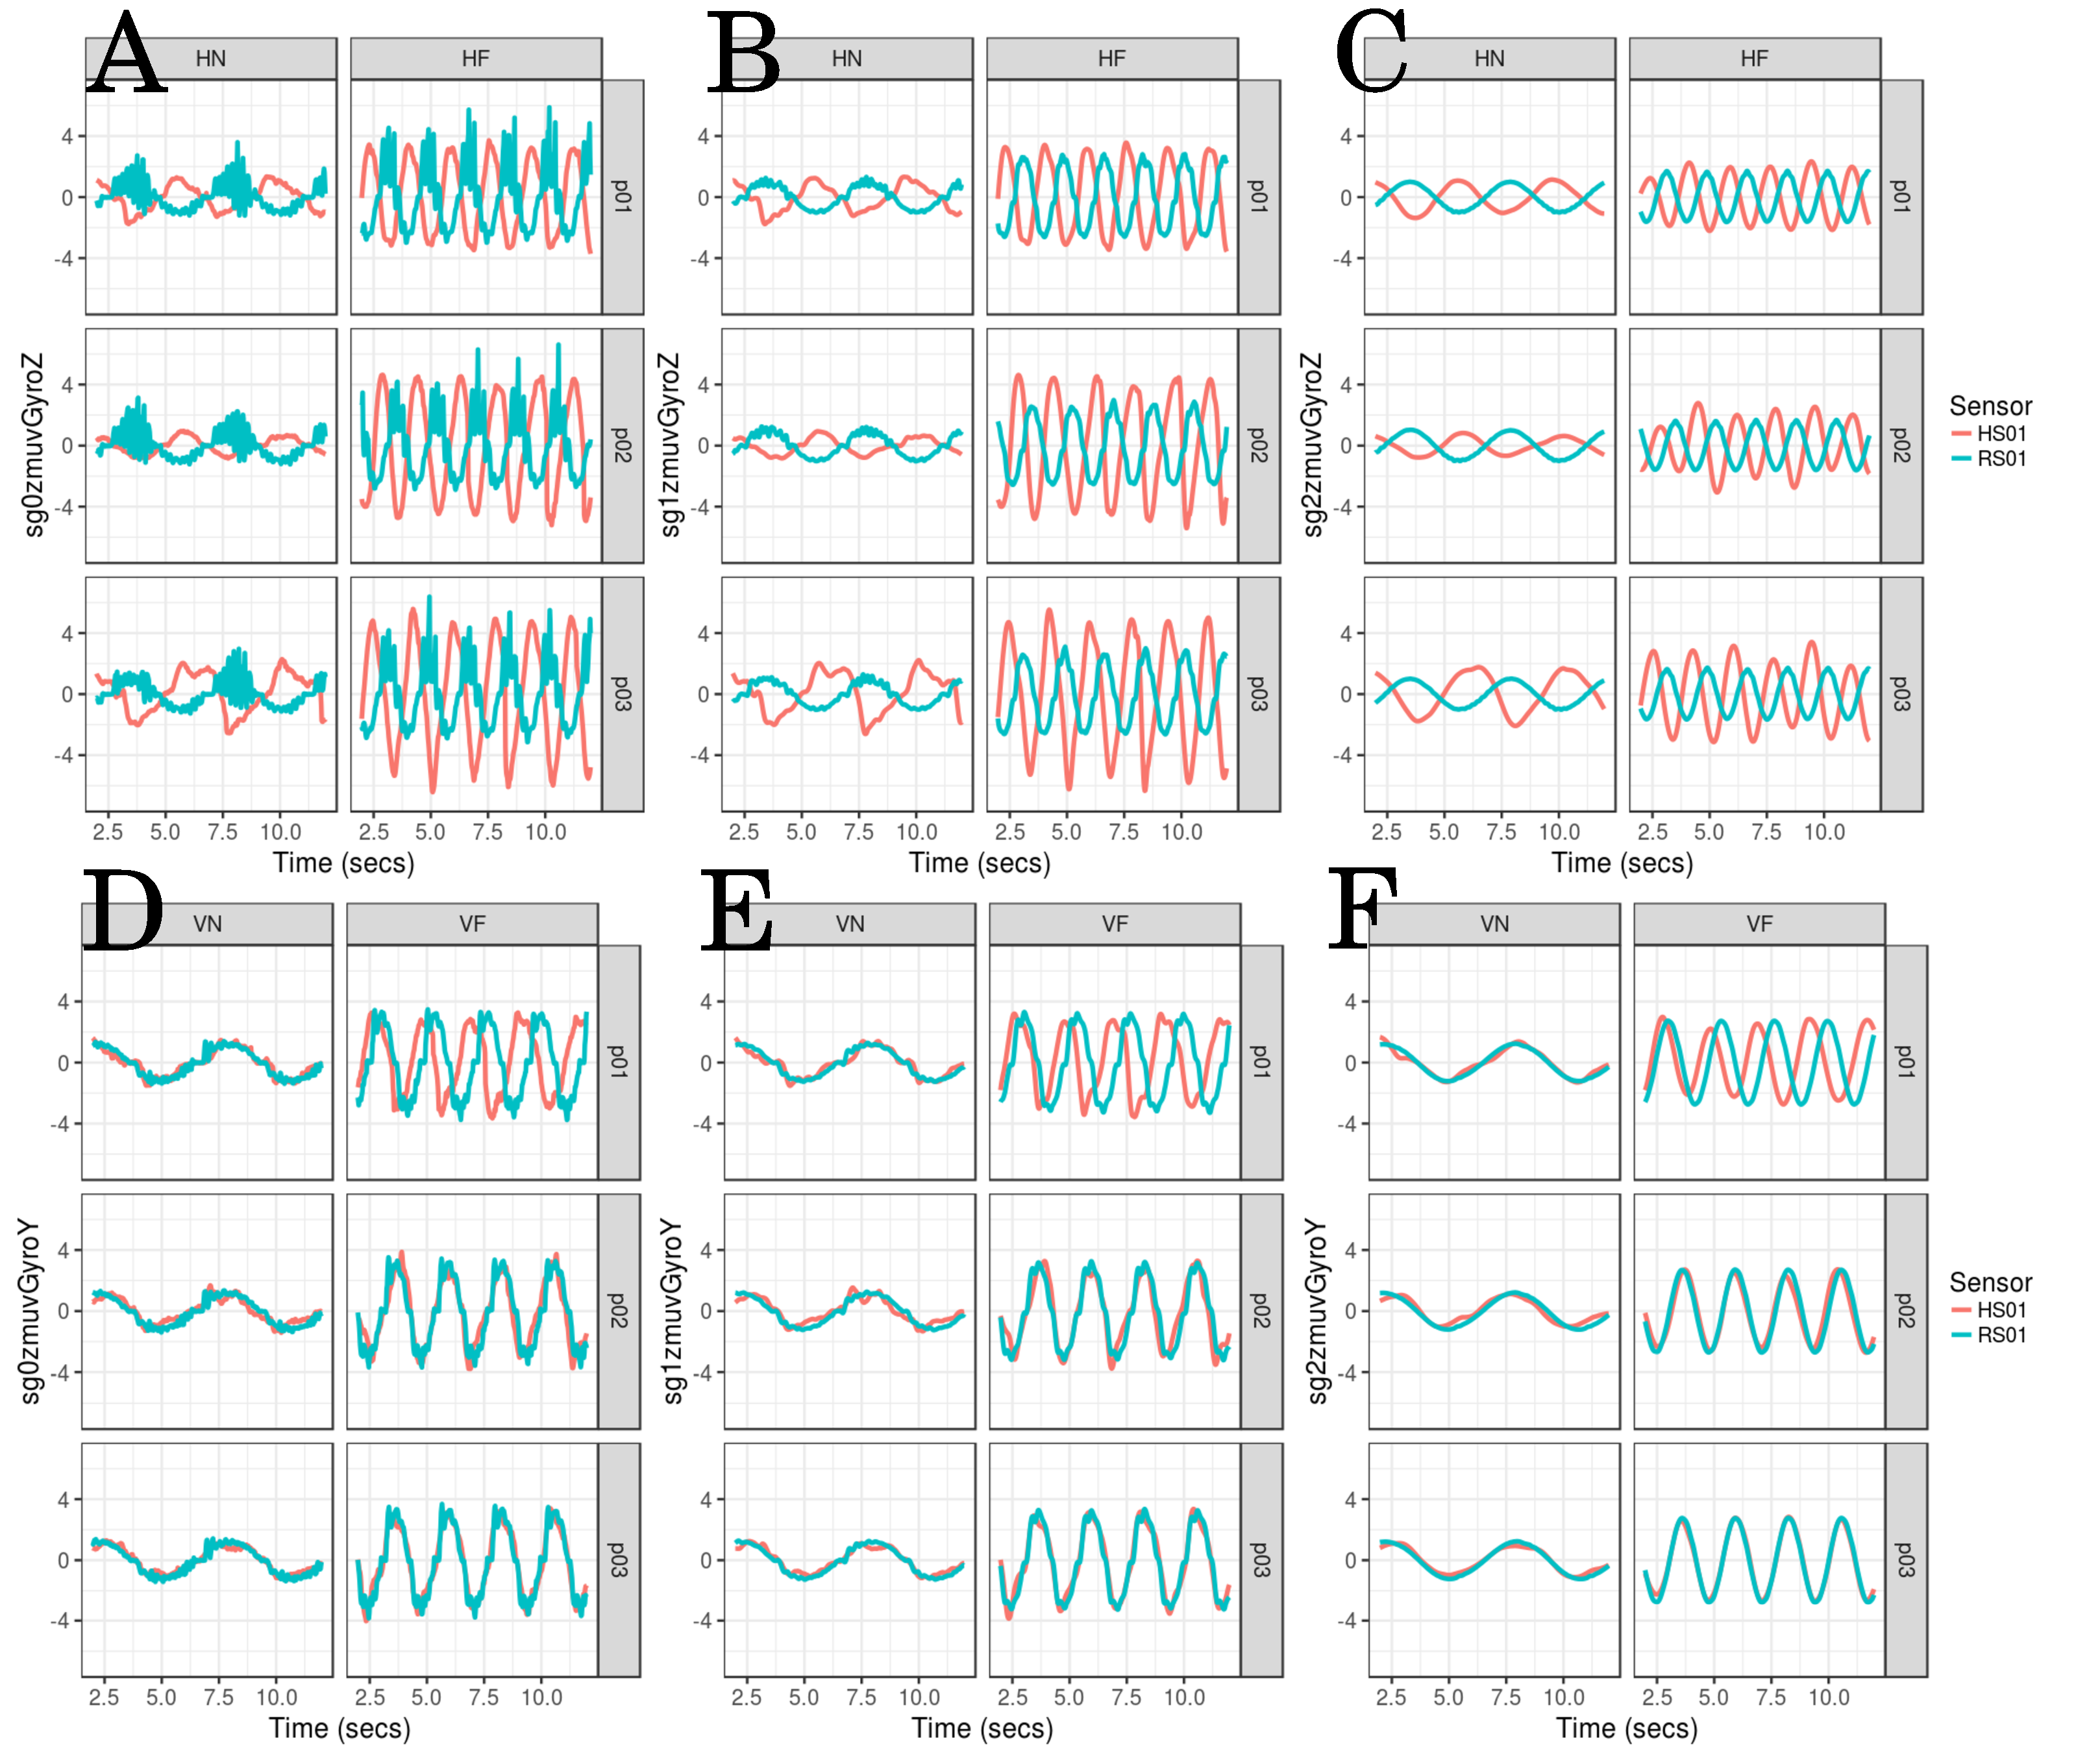
\includegraphics[width=1.0\textwidth]{figures/timeseries/pdf/fig1}
    	\caption{ 
	{\bf Time series for horizontal and vertical arm movements.}
		(A/D) raw-normalised (sg0zmuv), 
		(B/E) normalised-smoothed 1 (sg1zmuv) and
		(C/F) normalised-smoothed 2 (sg2zmuv).
		Time series are only for three participants 
		($p01$, $p02$, and $p03$) 
		for horizontal and vertical arm movements in normal 
		and faster velocity (HN, HF, VN, VF) 
		with the normalised GyroZ or GyroY axis 
		and with one sensor attached to the participant (HS01) 
		and other sensor attached to the robot (RS01).	
	Code and data to reproduce the figure is available from \cite{srep2019}.
        }
    \label{fig:ts}
\end{figure}
%%---------------------------------(FIGURE)------------------------------------




\subsubsection*{Raw data}
Considering the work of \cite{shoaib2016} which provided evidence of an 
improvement in recognition activities when combining data from 
accelerometer and gyroscope. We focus our analysis from data of the 
accelerometer and gyroscope of the NeMEMsi sensors \cite{Comotti2014} and 
leave the data of the magnetometer and quaternions for further investigation 
because of their possible variations with regard to magnetic disturbances.

Data from the accelerometer is defined by triaxial time series 
$A_x(n)$, $A_y(n)$, $A_z(n)$ which forms the matrix $\boldsymbol{A}$ 
(Eq.~\ref{eq:A}), and the same for data from the gyroscope 
which is defined by triaxial time-series of $G_x(n)$, $G_y(n)$, $G_z(n)$ 
representing the matrix $\boldsymbol{G}$ (Eq.~\ref{eq:G}).
Both triaxial time series of each sensor, $a$ and $g$, are denoted with 
its respective axes subscripts $x,y,z$, where $n$ is the sample index 
and $N$ is the same maximum length of all axes for the time series.
Matrices  $\boldsymbol{A}$ and $\boldsymbol{G}$ are represented as follows
%%---------------------------------(EQUATION)----------------------------------
\begin{equation}\label{eq:A}
\boldsymbol{A} =
\begin{pmatrix}
  A_x(n) \\
  A_y(n) \\
  A_z(n)
\end{pmatrix}
=
\begin{pmatrix}
 a_x(1),a_x(2),\dots,a_x(N) \\
 a_y(1),a_y(2),\dots,a_y(N) \\
 a_z(1),a_z(2),\dots,a_z(N) 
\end{pmatrix},
\end{equation}
%%---------------------------------(EQUATION)-----------------------------------
and 
%%---------------------------------(EQUATION)-----------------------------------
\begin{equation}\label{eq:G}
\boldsymbol{G} =
\begin{pmatrix}
 G_x(n) \\
 G_y(n) \\
 G_z(n)
\end{pmatrix}
=
\begin{pmatrix}
 g_x(1),g_x(2),\dots,g_x(N) \\
 g_y(1),g_y(2),\dots,g_y(N) \\
 g_z(1),g_z(2),\dots,g_z(N) 
\end{pmatrix}.
\end{equation}
%%---------------------------------(EQUATION)-----------------------------------




\subsubsection*{Postprocessing data}
After the collection of raw data from four NeMEMsi sensors,
time synchronisation alignment and interpolation were performed 
in order to create time series with the same length and synchronised time.
We refer the reader to \cite{Comotti2014} for further
details about the time synchronisation process.

\subsubsection*{Data normalization}
Data is normalised to have zero mean and unit variance 
using sample mean and sample standard deviation.
The sample mean and sample standard deviation using $x(n)$ is given by
%%---------------------------------(EQUATION)----------------------------------
\begin{equation}\label{eq:ms}
\mu_{x(n)}= \frac{1}{N} ( \sum_{i=1}^N x(i) ), \quad 
	\sigma_{x(n)} =  \sqrt{ \frac{  \sum_{1=1}^N ( x(i) - \mu_{x(n)} )^2 }{ N-1 }  },      
\end{equation}
%%---------------------------------(EQUATION)----------------------------------
and the normalised data, $\hat{x}(n)$, is computed as follows
%%---------------------------------(EQUATION)----------------------------------
\begin{equation}\label{eq:normalization}
\hat{x} (n) = \frac{   x(n) -  \mu_{x(n)}  }{   \sigma_{x(n)} }.   
\end{equation}
%%---------------------------------(EQUATION)----------------------------------

\subsubsection*{Smoothing data}
Commonly, a low-pass filter is the method either to capture the low 
frequencies that represent \%99 of the human body energy or to get 
the gravitational and body motion components of 
accelerations \cite{anguita2013}. However, for this work the elimination of 
certain range of frequencies is not the main focus but the conservation of 
the structure in the time series in terms of the width and heights where, 
for instance, Savitzky-Golay filter can help to accomplish 
such task \cite{press1992}. Savitzky-Golay filter is based on the 
principle of moving window averaging which preserves the area under 
the curve (the zeroth moment) and its mean position in time 
(the first moment) but the line width (the second moment) is violated 
and that results, for example, in the case of spectrometric data
where a narrow spectral line is presented with reduced height and width. 
With that in mind, the aim of Savitzky-Golay filtering is to find filter 
coefficients $c_n$ that preserve higher momentums which are based on local 
least-square polynomial approximations \cite{savitzkygolay1964, 
press1992, schafer2011}.
Therefore, Savitzky-Golay coefficients are therefore computed using 
an R function \texttt{sgolay(p,n,m)} where \texttt{p} is the filter order, 
\texttt{n} is the filter length (must be odd) and \texttt{m} is the 
$m$-th derivative of the filter coefficients  \cite{Rsignal}. 
Smoothed signal is represented with a tilde over the original 
signal: $\tilde{x}(n)$.

\subsubsection*{Window size data}
With regard to the window size, \cite{shoaib2016} investigated its effects 
using seven window lengths (2, 5, 10, 15, 20, 25, 30 seconds)
and combination of inertial sensors (accelerometer, gyroscope and linear 
acceleration sensor) to improve the activity recognition performance for 
repetitive activities (walking, jogging and biking) and less repetitive 
activities (smoking, eating, giving a talk or drinking a coffee).
With that in mind, Shoaib et al. \cite{shoaib2016} concluded that the 
increase of window length improve the recognition of complex activities 
because these requires a large window length to learn the repetitive 
motion patterns. Particularly, one of the recommendations is to use large 
window size to recognise less repetitive activities which mainly involve 
random hand gestures. Therefore, for the four activities 
(HN, HF, VN, and VF) in this work, which are mainly repetitive, 
we select only four window sizes for analysis: 2-s window (100 samples), 
5-s window (250 samples), 10-s (500 samples) and 15-s window (750 samples) 
(Fig~\ref{fig:sts}).









%% As a guideline references should be limited to 60 (this is not 
%% strictly enforced).
%\bibliography{sample}
%\bibliography{references}
\bibliography{../references/references}


\section*{Acknowledgements}

This work was funded by the University of Birmingham and the 
Mexican National Council of Science and Technology as part of 
Miguel Xochicale's PhD degree. I would like to thank to Dr. Dolores 
Columba Perez Flores and Prof. Martin J Russell for their helpful 
comments to polish the use of the language of mathematics and to 
Constantino Antonio Garcia Martinez et al. for developing the R 
package nonlinearTseries that help to accelerate the 
analysis of the nonlinear time series in this work.

\section*{Author contributions statement}
Contributions for this work of 
Miguel Xochicale (MX) and Chris Baber (CB) are as follows:
\begin{description}
\item[Conceptualisation] MX, CB
\item[Data Curation] MX
\item[Formal Analysis] MX
\item[Funding Acquisition] MX, CB
\item[Investigation] MX
\item[Methodology] MX
\item[Project Administration] MX
\item[Resources] CB
\item[Software] MX
\item[Supervision] CB
\item[Validation] MX
\item[Verification] MX
\item[Writing - Original Draft Preparation] MX
\item[Writing - Review] MX, CB
\item[Writing - Editing] MX
\end{description}

%
%\section*{Additional information}
%
%To include, in this order: \textbf{Accession codes} 
%(where applicable); \textbf{Competing interests} (mandatory statement). 
%
%The corresponding author is responsible for submitting a 
%\href{http://www.nature.com/srep/policies/index.html#competing}{competing interests statement} on 
%behalf of all authors of the paper. This statement must be included 
%in the submitted article file.
%
%\begin{figure}[ht]
%\centering
%\includegraphics[width=\linewidth]{stream}
%\caption{Legend (350 words max). Example legend text.}
%\label{fig:stream}
%\end{figure}

%\begin{table}[ht]
%\centering
%\begin{tabular}{|l|l|l|}
%\hline
%Condition & n & p \\
%\hline
%A & 5 & 0.1 \\
%\hline
%B & 10 & 0.01 \\
%\hline
%\end{tabular}
%\caption{\label{tab:example}Legend (350 words max). Example legend text.}
%\end{table}
%
%Figures and tables can be referenced in LaTeX using the ref command, 
%e.g. Figure \ref{fig:stream} and Table \ref{tab:example}.

\end{document}
